The MIT License (MIT)

Copyright (c) 2015 Donovan Squires

Permission is hereby granted, free of charge, to any person obtaining a copy
of this software and associated documentation files (the "Software"), to deal
in the Software without restriction, including without limitation the rights
to use, copy, modify, merge, publish, distribute, sublicense, and/or sell
copies of the Software, and to permit persons to whom the Software is
furnished to do so, subject to the following conditions:

The above copyright notice and this permission notice shall be included in all
copies or substantial portions of the Software.

THE SOFTWARE IS PROVIDED "AS IS", WITHOUT WARRANTY OF ANY KIND, EXPRESS OR
IMPLIED, INCLUDING BUT NOT LIMITED TO THE WARRANTIES OF MERCHANTABILITY,
FITNESS FOR A PARTICULAR PURPOSE AND NONINFRINGEMENT. IN NO EVENT SHALL THE
AUTHORS OR COPYRIGHT HOLDERS BE LIABLE FOR ANY CLAIM, DAMAGES OR OTHER
LIABILITY, WHETHER IN AN ACTION OF CONTRACT, TORT OR OTHERWISE, ARISING FROM,
OUT OF OR IN CONNECTION WITH THE SOFTWARE OR THE USE OR OTHER DEALINGS IN THE
SOFTWARE.


\documentclass{article}
\usepackage{setspace}

\usepackage{graphicx,calc,pdfpages}	% package that allows graphics to be included
% sets 1.5in margins instead of article's large defaults
\usepackage[letterpaper,margin=1.5in]{geometry}
\usepackage{indentfirst}		% indents the first paragraph of sections

\usepackage{float}			% required for [H] option of \begin{figure}
\usepackage{caption,subcaption}
\usepackage{longtable,pdflscape}
\usepackage{amsmath}
\usepackage[hidelinks]{hyperref}

\usepackage{appendix}			% additional appendix formatting options

% render units in upright text (non-italics) in math mode (e.g. $20\unit(Hz)$)
\newcommand{\unit}[1]{\ensuremath{\, \mathrm{#1}}}

\doublespacing

\begin{document}

\pagenumbering{alph}			% abstract and copyright page not numbered
					% using lower case letters for pdf pagination
%The MIT License (MIT)

Copyright (c) 2015 Donovan Squires

Permission is hereby granted, free of charge, to any person obtaining a copy
of this software and associated documentation files (the "Software"), to deal
in the Software without restriction, including without limitation the rights
to use, copy, modify, merge, publish, distribute, sublicense, and/or sell
copies of the Software, and to permit persons to whom the Software is
furnished to do so, subject to the following conditions:

The above copyright notice and this permission notice shall be included in all
copies or substantial portions of the Software.

THE SOFTWARE IS PROVIDED "AS IS", WITHOUT WARRANTY OF ANY KIND, EXPRESS OR
IMPLIED, INCLUDING BUT NOT LIMITED TO THE WARRANTIES OF MERCHANTABILITY,
FITNESS FOR A PARTICULAR PURPOSE AND NONINFRINGEMENT. IN NO EVENT SHALL THE
AUTHORS OR COPYRIGHT HOLDERS BE LIABLE FOR ANY CLAIM, DAMAGES OR OTHER
LIABILITY, WHETHER IN AN ACTION OF CONTRACT, TORT OR OTHERWISE, ARISING FROM,
OUT OF OR IN CONNECTION WITH THE SOFTWARE OR THE USE OR OTHER DEALINGS IN THE
SOFTWARE.

%preamble copies main document for testing
%comment when including in main doc.
%=============================================
% \documentclass{article}
% \usepackage{setspace}
% \usepackage{graphicx,calc,pdfpages}
% \usepackage[letterpaper,margin=1.5in]{geometry}
% \usepackage{indentfirst}
% \usepackage{float}
% \usepackage{caption,subcaption}
% \usepackage{longtable,pdflscape}
% \usepackage{amsmath}
% \usepackage[hidelinks]{hyperref}
% \usepackage{appendix}

% \doublespacing

% \begin{document}
%=============================================




\begin{centering}
\begin{singlespace}
	INSTRUMENTATION ELECTRONICS FOR AN INTEGRATED \\ ELECTROPHYSIOLOGY DATA ACQUISITION \\ AND STIMULATION SYSTEM
		
	\vspace{2\baselineskip}
%	\vfill
	
	Donovan Squires, M.S.E.\\
	\vspace{\baselineskip}
	Western Michigan University, 2013
\end{singlespace}	
\end{centering}

\vspace{0.5\baselineskip}

The Neurobiology Engineering Laboratory at Western Michigan University has need of an electrophysiology instrumentation system combining generation of multiple arbitrary stimulation waveforms and recording of action potentials on multiple channels.  Electronics for an instrumentation system with the capability of generating four unique stimulation waveforms and recording action potentials on eight channels were developed and implemented on a printed circuit board.  Collaboration with fellow graduate student, Mr.~Kyle Batzer, who developed firmware and software for the instrumentation system as described in his thesis, was essential for successful realization of the instrumentation system.  Knowledge gained and reported by previous students working in the Neurobiology Engineering laboratory also contributed to the development.  This system was used to perform a standard electrophysiology
experiment on earthworm giant axon action potentials using only instrumentation electronics and software developed by students at Western Michigan University.




%=============================================
% \thispagestyle{empty}	
% \end{document}
	% leave out of GitHub until I get permission from Dr. Miller
\thispagestyle{empty}

\newpage
\pagenumbering{roman}			% use lowercase roman numerals for frontmatter
					% restarts counter, title page is "i" even though
					% page number isn't visible

The MIT License (MIT)

Copyright (c) 2015 Donovan Squires

Permission is hereby granted, free of charge, to any person obtaining a copy
of this software and associated documentation files (the "Software"), to deal
in the Software without restriction, including without limitation the rights
to use, copy, modify, merge, publish, distribute, sublicense, and/or sell
copies of the Software, and to permit persons to whom the Software is
furnished to do so, subject to the following conditions:

The above copyright notice and this permission notice shall be included in all
copies or substantial portions of the Software.

THE SOFTWARE IS PROVIDED "AS IS", WITHOUT WARRANTY OF ANY KIND, EXPRESS OR
IMPLIED, INCLUDING BUT NOT LIMITED TO THE WARRANTIES OF MERCHANTABILITY,
FITNESS FOR A PARTICULAR PURPOSE AND NONINFRINGEMENT. IN NO EVENT SHALL THE
AUTHORS OR COPYRIGHT HOLDERS BE LIABLE FOR ANY CLAIM, DAMAGES OR OTHER
LIABILITY, WHETHER IN AN ACTION OF CONTRACT, TORT OR OTHERWISE, ARISING FROM,
OUT OF OR IN CONNECTION WITH THE SOFTWARE OR THE USE OR OTHER DEALINGS IN THE
SOFTWARE.

%preamble copies main document for testing
%comment when including in main doc.
%=============================================
% \documentclass{article}
% \usepackage{setspace}
% \usepackage{graphicx,calc,pdfpages}
% \usepackage[letterpaper,margin=1.5in]{geometry}
% \usepackage{indentfirst}
% \usepackage{float}
% \usepackage{caption,subcaption}
% \usepackage{longtable,pdflscape}
% \usepackage{amsmath}
% \usepackage[hidelinks]{hyperref}
% \usepackage{appendix}

% \doublespacing

% \begin{document}
%=============================================


\begin{singlespace}
\begin{centering}

	INSTRUMENTATION ELECTRONICS FOR AN INTEGRATED \\ ELECTROPHYSIOLOGY DATA ACQUISITION \\ AND STIMULATION SYSTEM

	
	\vspace{6\baselineskip}
%	\vfill
	
	by\\
	\vspace{\baselineskip}
	Donovan Squires
	
%	\vspace{10\baselineskip}
	\vfill
	
	A thesis submitted to the Graduate College \\ in partial fulfillment of the requirements \\ for the degree of Master of Science in Engineering (Electrical) \\ Electrical and Computer Engineering \\ Western Michigan University \\ December 2013 
	
%	\vspace{9\baselineskip}
	\vfill
	
\end{centering}

Thesis Committee:\\ \\
\hspace*{0.5in} Damon A.~Miller, Ph.D., Chair\\
\hspace*{0.5in} Bradley J.~Bazuin, Ph.D.\\
\hspace*{0.5in} Frank L.~Severance, Ph.D.\\



\end{singlespace}

%=============================================
% \thispagestyle{empty}	
% \end{document}

\thispagestyle{empty}			% removes page number (must be after \maketitle, if using)

\newpage

\pagenumbering{alph}
\addtocounter{page}{1}			% counter restarted, so have to add 1

\null
\vfill

\begin{noindent}
\begin{singlespace}
\begin{centering}

Copyright \copyright~2013 by Donovan Squires.

\medskip

\href{http://creativecommons.org/licenses/by/3.0/}{
\includegraphics{./figures/by}}

\medskip
 
Except where otherwise noted, this work is licensed under the Creative Commons Attribution 3.0 Unported License. To view a copy of this license, visit \url{http://creativecommons.org/licenses/by/3.0/}.

\bigskip

Foreword is Copyright \copyright~2013 by Damon A. Miller.  All rights reserved.

\bigskip

Some names in this thesis are trademarks.  Lack of a trademark symbol does not imply that a name is not a trademark

\end{centering}
\end{singlespace}
\end{noindent}
\thispagestyle{empty}

\newpage

\pagenumbering{roman}
\addtocounter{page}{1}			% counter restarted, so have to add 1

\section*{Foreword} 			%'*' keeps the section from being numbered
%\addcontentsline{toc}{section}{Introduction} %add un-numbered section to table of contents

\input{miller/SquiresBatzerThesisForeword.tex}

\newpage

\tableofcontents

\newpage

\listoffigures

\newpage

\listoftables

\newpage

\pagenumbering{arabic}			% switch to arabic page number, reset page counter to 1

\section[Introduction]{Introduction\footnote{This section is co-authored with Kyle Batzer,~\cite{BatzerMSEE}.}\addtocounter{footnote}{-1}\addtocounter{Hfootnote}{-1}}

%brief overview of MEA and Earthworm and the need for a 
%custom eight channel Stimulation and Data Acquisition System
An Integrated Electrophysiology Data Acquisition and Stimulation System to support electrophysiology research has been developed by building on previous work at WMU~\cite{ArmstrongSD,CarusoDaiekJones,StahlMSEE,BatzerCorsiCrampton,EllingerMSEE}, studying commercial systems~\cite{MCSystems}, and reviewing the research literature~\cite{Potter2005,Jimbo2003,Blum2007}.  The developed prototype provides a real-time platform for measurement and stimulation of biological electrical activity and a PC application for controlling the real-time platform and visualizing cellular activity.  The system can accommodate up to eight measurement channels and four stimulation channels, and the design can be expanded for up to 64 channels to support future research at the Western Michigan University (WMU) Neurobiology Engineering Laboratory.
 
The developed prototype is viable for a wide array of electrophysiology experiments, completely fulfilling the instrumentation needs of~\cite{Olivo,KuehJellies,Kladt2010} and partially fulfilling the requirements for~\cite{Marom02,DeMarse04,Potter2005}.  In particular, a standard electrophysiology experiment was performed on earthworm giant axon action potentials to validate system functionality.  The prototype is also intended for studying software and hardware principles required for performing research using cells cultured on a Microelectrode Array (MEA), e.g.~\cite{MCSystems}.  A cell culture protocol has been developed~\cite{EllingerMSEE} and previous work on such a system~\cite{ArmstrongSD,CarusoDaiekJones,BatzerCorsiCrampton}, including low noise amplification, has been completed~\cite{StahlMSEE}.  Initial analytical algorithms have also been developed~\cite{EllingerMSEE}.


\section[Specifications]{Specifications\footnotemark}\label{sec:spec}

%\section{Specifications}

%[This is a list of specifications for the combined software and hardware.  It might be better understood if these were called "requirements"]

The Data Acquisition and Stimulation System (DASS) is expected to provide to following functionality:

\begin{enumerate}

\item Provide a platform for performing electrophysiology experiments with earthworms as described in~\cite{Olivo,KuehJellies}

	\begin{enumerate}
	
	\item Produce a voltage-controlled square wave stimulation pulse with widths from 0.01ms to 100ms and amplitudes from 0.1V to 10V
	
	\item Produce single stimulation pulses or multiple pulses at rates from 1Hz to 10Hz
	
	\item Provide at least one differential recording channel
	
	\item Record an action potential voltage from the time of a stimulation pulse for a minimum duration of 20ms
	
	\item Plot the recorded voltage
	
	\item Store the recorded voltage to a non-proprietary, standard file format
	
	\end{enumerate}
	

\item Provide a platform for stimulation and recording of neuron cell culture electrical activity via MEA electrodes

	\begin{enumerate}
	
	\item Provide at least four recording channels
	
	\item Store data from recording channels continuously
	
	\item Provide at least four voltage-controlled arbitrary stimulation channels
	
	\item Output single-ended stimulation signals on recording electrodes and add culture voltage offset to the stimulation signal
	
	\item Provide an interface that can specify stimulation waveforms, locations, and intervals that can be updated based on data from the recording electrodes
	
	\end{enumerate}

\item Utilize Low-Noise Amplifier described in~\cite{StahlMSEE}

	\begin{enumerate}
	
	\item Connect to each Low-Noise Amplifier channel with a PCI-Express card edge connector
	
	\item Provide $\pm 7\unit{V}$ to $\pm 15\unit{V}$ analog voltage supplies and ground via the card edge connector
	
	\item Provide ability to independently switch four digital inputs for each channel, $0_{\mathrm{IH}}=0.8\unit{V}$ and $1_{\mathrm{IL}}=2.4\unit{V}$
	
	\item Route differential analog input to the card edge connector for each channel
	
	\item Convert the 20Hz to 14.6kHz analog output signal~\cite{StahlMSEE} to digital samples %with a resolution better than (XX)$V/LSB$ [check with references or base number on oscilloscope resolution]
	
	\item Route a single-ended stimulation signal to each channel
	
	\end{enumerate}
	
\item Additional requirements

	\begin{enumerate}
	
%	\item Produce arbitrary stimulation waveforms with minimum bandwidth (XX)$Hz$ and minimum slew rate (XX)$V / \mu s$
	
	\item Employ proven, effective circuit design and layout best practices
	
%	[Anything else that doesn't fit in the above categories]
	
	\end{enumerate}
	
\end{enumerate}


\section{Terminology}\label{sec:term}

\paragraph{Analog to Digital Converter (ADC)} A device for converting an analog voltage to a digital code.  The ADC on the Electrophysiology Interface is an Analog Devices AD7606.

\paragraph{Complex Programmable Logic Device (CPLD)} Non-volatile programmable logic device that is used to allow limited outputs from the FPGA to control many more digital input lines required by multiple Preamp boards connected to the Electrophysiology Interface.  The CPLD on the Electrophysiology Interface may be a Xilinx\textsuperscript{\textregistered} XC9536XL or a XC9572XL (the devices are pin compatible).

\paragraph[Data Acquisition and Stimulation System \(DASS\)]{Data Acquisition and Stimulation System (DASS)\footnote{This item is co-authored with Kyle Batzer,~\cite{BatzerMSEE}.}\addtocounter{footnote}{-1}\addtocounter{Hfootnote}{-1} }  System intended for electrophysiology experiments described in this thesis and corresponding thesis~\cite{BatzerMSEE}.  The DASS includes all hardware, software, and firmware.

\paragraph[Data Acquisition and Simulation Control Center \(DASCC\)]{Data Acquisition and Simulation Control Center (DASCC)\footnotemark}  PC application, described in~\cite{BatzerMSEE}, for controlling and transferring data to and from the RTSC.

\paragraph{Differential Output Amplifier} A custom designed operational amplifier configuration on the Electrophysiology Interface that provides gain and offset to an input from the DAC and provides two output signals where one signal is the inverse of the other signal, with respect to ground (0V).

\paragraph{Digital to Analog Converter (DAC)} A device for converting a digital code to an analog voltage.  The DAC on the Electrophysiology Interface is an Analog Devices AD5678.

\paragraph[Electrophysiology Interface]{Electrophysiology Interface\footnote{This item is co-authored with Kyle Batzer,~\cite{BatzerMSEE}.}\addtocounter{footnote}{-1}\addtocounter{Hfootnote}{-1}}  Subsystem that provides the RTSC with an interface to biological systems.  It consists of a custom PCB described in this thesis.

\paragraph{Field Programmable Gate Array (FPGA)} Volatile programmable logic device that performs the majority of the real time control functions on the RTSC.  The FPGA on the RTSC is a Xilinx\textsuperscript{\textregistered} Spartan-3 XC3S500E.

\paragraph[Real Time System Controller \(RTSC\)]{Real Time System Controller (RTSC)\footnotemark\addtocounter{footnote}{-1}\addtocounter{Hfootnote}{-1}}  Subsystem that implements the real-time functions of the system.  It consists of a Digilent\textsuperscript{\textregistered} Nexys\textsuperscript{TM} 2 development board~\cite{DigilentNexys2rm,DigilentNexys2sch}, with custom firmware described in~\cite{BatzerMSEE}.

\paragraph[Preamp]{Preamp\footnotemark}  Low noise instrumentation amplifier with stimulation dc bias addition for MEA experiments.  Designed by Mr. John Stahl as described in~\cite{StahlMSEE}.  

\paragraph{Printed Circuit Board (PCB)} A fiberglass board with thin layers of copper that are etched and drilled allowing electronic components to be mounted and connected in a compact, professional-looking package for an electronic circuit.






\section{Data Acquisition and Stimulation System Hardware}\label{sec:hardware}

%Overview of the stimulation and acquisition hardware including custom board and relevant sections of the Nexys2 development board as shown in Figure~\ref{fig:System}.  Detailed description of each item of the system in the following subsections.
%\ref command will put in the figure number if latex can't find the label it will instead put in "??"
A digital platform that interfaces with analog signals is an effective and flexible instrumentation strategy for electrophysiology experiments that require arbitrary stimulation signals and recording action potentials.  A digital to analog converter (DAC) can convert a digitally represented waveform to an analog signal that can be used to stimulate experimental subjects, and a analog to digital converter (ADC) can convert analog voltages to digital data that can be saved in readily available digital formats.

The user interface of the platform needs to be flexible to accommodate the various electrophysiology experiments it will perform.  Custom PC software allows the user to control the complex capabilities of the platform while also providing access to data storage space; however, PC hardware is not capable of interfacing directly with DAC and ADC circuits.  To save development complexity, real time control of the DAC and ADC is accomplished with a Digilent\textsuperscript{\textregistered} Nexys\textsuperscript{TM} 2 field-programmable gate array (FPGA) development board.  The DAC and ADC, along with related circuitry, are implemented on a custom designed printed circuit board (PCB).

An overview of the Data Acquisition and Stimulation System (DASS) is shown in Figure~\ref{fig:System}.  Custom user interface software on the PC communicates to the Digilent\textsuperscript{\textregistered} Nexys\textsuperscript{TM} 2 Real Time System Controller (RTSC) board over USB and serial RS232 interfaces.  An RS232 level converter chip converts the PC's RS232 logic levels to FPGA compatible TTL logic levels and vice-versa.  A microcontroller on the RTSC provides the USB physical layer (PHY) and is capable of controlling the Joint Test Action Group (JTAG) bus to load a FPGA configuration file into the FPGA or save the configuration to a flash memory device capable of storing the configuration on the board without power and loading the configuration into the FPGA upon power-up.  The JTAG bus also allows a configuration to be loaded into the Complex Programmable Logic Device (CPLD), which can be programmed with logic to allow the FPGA to control the multiple digital inputs on the Preamp boards with fewer output pins.  A DRAM chip on the RTSC stores stimulation waveform data.  The FPGA outputs stimulation waveform data to the DAC on the Electrophysiology Interface board and controls the ADC.  Data from the ADC is sent to the microcontroller, which has customized firmware that transfers data to the PC over the USB interface.

\begin{landscape}
\begin{figure} % [H] option tell Latex to place the figure at this place in the document
	\begin{singlespace}
	\centering	
		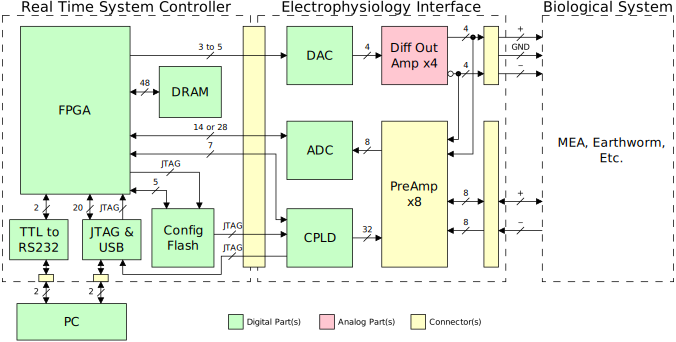
\includegraphics{./figures/System}
		% Tells (pdf)latex to look for graphic: System.*
		% running pdflatex will include System.pdf and running latex will include System.eps	
	\caption{The Data Acquisition and Stimulation System consists of a PC, the Real Time System Controller Board, which is a Digilent\textsuperscript{\textregistered} Nexys\textsuperscript{TM} 2 FPGA development board~\cite{DigilentNexys2rm,DigilentNexys2sch}, and the Electrophysiology Interface board, which is based on previous work as described in the text.\label{fig:System}}
	% \label{} allows this figure to be referenced in the text and it must be immediately after or in \caption{}
	\end{singlespace}
\end{figure}
\end{landscape}

The analog operating ranges of the DAC and ADC are not compatible with the voltages used in electrophysiology experiments, so a differential output amplifier circuit conditions the DAC output, and connectors are provided to allow previously developed low-noise amplifier boards~\cite{StahlMSEE} (Preamp) to condition low-voltage action potentials for input into the ADC.  The Preamp boards have the capability of outputting a provided analog stimulation signal on the recording electrode; digital inputs control whether the Preamp is in stimulation or recording mode.

Typical use of the DASS involves the following: connecting the Electrophysiology Interface board stimulation and data acquisition channels to the biological portion of the electrophysiology experimental setup; powering the Electrophysiology Interface and RTSC boards, which causes the FPGA to be configured based on the data in the flash memory configuration chip; using the PC application to send commands over the RS232 interface to the FPGA for configuring the stimulation and data acquisition channels~\cite{BatzerMSEE}; running a script on the PC application that sends commands to the FPGA over the RS232 interface to load stimulation waveform profiles in the DRAM, sets the Preamp boards to stimulation or recording mode, causes the DAC to output the stimulation waveform, collects data from the ADC, and transfers data collected from the ADC to the PC for storage and analysis~\cite{BatzerMSEE}.  Waveforms from the DAC output are amplified and conditioned by the Differential Output Amplifier before being routed to the biological system either to independent stimulation electrodes or through the Preamp boards to the recording electrodes.  The response from the biological system is observed on the recording electrodes as analog electrical signals which are routed to the Preamp boards for amplification and filtering before being routed to the ADC for conversion to digital information.

This thesis describes the relevant circuitry on a Digilent\textsuperscript{\textregistered} Nexys\textsuperscript{TM} 2 FPGA development board that is necessary to implement a RTSC board, and it describes the design of the Electrophysiology Interface board.  The design of the PC software, microcontroller firmware, and programmable logic configurations is described in~\cite{BatzerMSEE}.



\subsection{Power Supply}\label{sec:power}

%Design and description of power sources and voltage regulators
The hardware for the Data Acquisition and Stimulation System requires several supply voltages to power the digital integrated circuits (ICs) in addition to dual analog power supplies for amplification circuitry.  Consequently, there are several options for providing power to the Real Time System Controller Board and Electrophysiology Interface board.  Figure~\ref{fig:Power} summarizes the power needs of the ICs and circuit blocks along with the power input connectors and voltage regulators.

\begin{figure}[H]
	\begin{singlespace}
	\centering 
		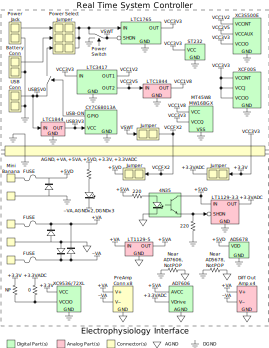
\includegraphics{./figures/Power} 
	\caption{Power connectors and IC power connections on the Real Time System Controller Board~\cite{DigilentNexys2rm,DigilentNexys2sch} and the Electrophysiology Interface board\label{fig:Power}}
	\end{singlespace}
\end{figure}

\subsubsection{Real Time System Controller Power}\label{sec:rtscpower}

The RTSC has selectable input power options configured by placing a jumper connecting the desired power connector to a LTC1765 switching voltage regulator.  The power jack and battery connector both connect directly to the regulator, but the CY7C68013A Cypress microcontroller, which requires a $+3.3\unit{V}$ supply and acts as the USB PHY, draws power exclusively from the USB interface, so a LTC1844 linear regulator is included to regulate the $+5.0\unit{V}$ USB input voltage to the required value.  When a USB cable is connected to the RTSC and a PC, the Cypress microcontroller informs the PC that more than $100\unit{mA}$ of current will be drawn over the USB interface; then, the USB$-$ON signal switches a NMOS transistor, connecting USB power, which can supply up to $500\unit{mA}$ of current, to the power selection jumper~\cite{DigilentNexys2rm,DigilentNexys2sch}.  The power consumption of the RTSC will vary based on the configuration of the Xilinx\textsuperscript{\textregistered} XC3S500E FPGA, clock speeds of the digital logic, and the power drawn from the Electrophysiology Interface board~\cite{DigilentNexys2rm}.

The power switch on the RTSC board connects the active low shutdown signal ($\overline{\mathrm{SHDN}}$) of the LTC1765 regulator to either the power selection jumper (to enable the regulator output) or to ground (to disable the regulator output)~\cite{LT1765ds}.  Setting the power switch to the off position does not disconnect USB power from the Cypress microcontroller but does disconnect the main power jumper from VCCFX2 if the jumper is in place to connect the VSWT to VCCFX2~\cite{DigilentNexys2sch}.

Most of the circuits on the RTSC board are powered by the VCC3V3 supply, which is why a LTC1765 high-efficiency switching regulator is used for the supply.  The ST232 RS232 level shifting IC and the Xilinx\textsuperscript{\textregistered} Platform Flash XCF00S configuration flash memory require only 3.3V~\cite{ST232ds,XilinxPlatformFlashDS}.  The Xilinx\textsuperscript{\textregistered} Spartan 3E XC3S500E FPGA requires a significant amount of current at $+1.2\mathrm{V}$ for its internal core, VCCINT, and requires $+2.5\unit{V}$ for its auxiliary supply voltage, VCCAUX, so a LTC3417 high-efficiency dual-output switching regulator provides the needed supply voltages~\cite{DigilentNexys2rm,Spartan3eDS}.  Also, the MT45W8MW16BGX 128Mb DRAM module alone requires a $1.8\unit{V}$ core voltage, with a maximum current of $25\unit{mA}$ at $66\unit{MHz}$ and $45\unit{mA}$ at $133\unit{MHz}$, along with an IO voltage supply equal to the FPGA IO voltage~\cite{MicronDRAMds}.  Thus, a LTC1844 linear regulator is provided for the specialized VCC1V8 voltage supply, and since linear regulator efficiency is directly proportional to the magnitude of the voltage drop across the regulator, it is powered by the voltage supply that will require the least voltage drop, VCC2V5~\cite{DigilentNexys2sch}.

\subsubsection{Electrophysiology Interface Power}

To isolate analog devices from the noise generated by digital devices, it is preferable to have separate power supplies and ground for the digital and analog devices on the Electrophysiology Interface board.  In addition, the Preamp boards connected also draw power from the analog voltage supplies on the Electrophysiology Interface board.

The integrated circuits requiring a digital voltage supply are the Analog Devices AD5678 DAC, the Xilinx\textsuperscript{\textregistered} XC9536/72XL CPLD, and the logic supply, VDrive, of the AD7606 ADC.  The nine LT1124 dual op-amp ICs of the differential output amplifier blocks require dual analog voltage supplies, and each Preamp requires dual analog voltage supplies for its LT1167 instrumentation amplifier, LT1124 dual op-amp, LT1125 quad op-amp, and ADG202 analog switch ICs.  Complicating the analog voltage supply requirements is the Analog Devices AD7606 ADC, which requires a $+5.0\mathrm{V} \pm 0.25\unit{V}$ analog voltage supply, AVCC~\cite{AD7606ds}.

Five 2mm banana (also known as mini-banana) connectors are provided on the Electrophysiology Interface board to connect analog voltage ($\pm \mathrm{VA}$) and ground (AGND) and digital voltage (+5VD) and ground (DGND).  The magnitude of +VA should be a close as possible to the magnitude of $-\mathrm{VA}$.  Table~\ref{tab:powerinput} shows the acceptable voltage range of the power supply inputs.  The minimum and maximum values of +5VD are determined by the AD5678 requirements, but it should be noted that the maximum DAC output voltage will be equal to the supply voltage~\cite{AD5678ds}.  The minimum value for the $\pm \mathrm{VA}$ supply is determined by the dropout voltage of the LT1129-5 regulator ($0.45\unit{V}$ at $100\unit{mA}$ load current~\cite{LT1129ds}), and the maximum value for the $\pm \mathrm{VA}$ supply is limited by the requirements of the LT1167 instrumentation amplifier and ADG202 analog switches on the Preamp boards~\cite{LT1167ds,ADG202Ads}.

\renewcommand{\arraystretch}{1.3}
\begin{table}[h]
\centering
\begin{tabular}{|l|l|l|l|}
\hline
Supply & TYP (V) & MIN (V) & MAX (V)\\
\hline
+5VD & 5.0 & 4.5 & 5.5\\
\hline
$|\pm \mathrm{VA}|$ & 9.0 & 5.5 & 15.0\\
\hline
\end{tabular}
\caption{Electrophysiology Interface power supply voltages\label{tab:powerinput} }

\end{table}
\renewcommand{\arraystretch}{1.0}

Fuses and protection diodes will protect the circuits on the Electrophysiology Interface board if the supply leads are reversed.  If the supply leads are reversed, one or more of the protection diodes will be forward biased, allowing a large amount of current to flow between the reversed supply leads causing a fuse to blow and the dangerous voltage to be disconnected from the rest of the board.  The fuses on the Electrophysiology Interface board are surface mount fuses in 0805 packages that have the advantage of taking up very little board space but have the disadvantage of having a high series resistance of $0.7\unit{\Omega}$ (measured).  When one of the fuses blows, it is not visually distinguishable from a non-blown fuse.  To ensure a low resistance connection, the ground connection does not go through a fuse, which will present a problem if a power lead is connected to a ground connector that creates a large voltage difference between the analog and digital grounds.

The $3.3\unit{V}$ supply from the RTSC board is used to power the core of the CPLD and may be used to power the IO buffers of the CPLD and ADC by connecting the jumper from $+3.3\unit{V}$ to +3.3VADC, in which case the LT1129-3.3 should not be populated.  Alternatively, the IO buffer of both the ADC and CPLD or the ADC alone may be powered by a LT1129-3.3 linear regulator that converts the +5VD voltage to $3.3\unit{V}$.  To ensure that the IO buffers of the ADC are powered only when the ADC's AVCC is powered and to preserve analog and digital isolation, a 4N35 opto-isolator, with its input driven by the $+5\mathrm{VA}$ supply, controls the operation of the linear regulator.  Since other signals from the CPLD and DAC violate analog and digital isolation, as discussed in section~\ref{sec:ground}, the opto-isolator is excessive, but it illustrates the concept of analog and digital isolation.

Both the AD5678 DAC and the AD7606 ADC recommend analog and digital ground and power isolation, but when analog and digital grounds are to be connected at some point, the connection should be as close as possible to the AD5678 as recommended by~\cite{AD5678ds}, and the connection should be as close as possible to the AD7606 as recommended by~\cite{AD7606ds}.  To accommodate this conflicting information, pads for $0\unit{\Omega}$ resistors are provided near the DAC and ADC for testing analog and digital ground connections.  Although, with all of the signals that connect analog and digital powered devices, as discussed in section~\ref{sec:ground}, a single $0\unit{\Omega}$ resistor may not be sufficient for routing signal return currents.

The +5VD supply may be configured to be powered by the main input bus of the RTSC board by connecting the jumper on the RTSC the connects VSWT to VCCFX2 and the jumper on the Electrophysiology Interface board that connects VCCFX2 to +5VD.  The reverse should not be practiced: using +5VD to power the RTSC could result in the +5VD power supply being shorted to ground by the power switch that connects VSWT to the main input bus or to ground.  If the USB interface is used to power the RTSC and the Electrophysiology Interface boards, care must be taken to ensure that no more than $500\unit{mA}$ is drawn from the USB interface.  A typical configuration of the FPGA may cause the RTSC, itself, to draw $300\unit{mA}$ of power from the USB interface~\cite{DigilentNexys2rm}.  The AD5678 draws only $2.6\unit{mA}$ of quiescent current with its internal voltage reference on, but the AD5678 output amplifiers draw varying amounts of current based on input resistance of the Differential Output Amplifier blocks~\cite{AD5678ds}.  The CPLD's power consumption varies depending on its configuration and clock speed.  With a configuration consisting entirely of 16-bit counters, a XC9536XL can draw between $15\unit{mA}$ and $65\unit{mA}$ of current from the $+3.3\unit{V}$ power supply, and a XC9572XL can draw between $25\unit{mA}$ and $125\unit{mA}$~\cite{XC9536XLds,XC9572XLds}.  The resulting current drawn from the USB interface depends on the power efficiency of the LTC1765, which varies from 75\% to 87\% depending on output current~\cite{LT1765ds}.

LEDs are provided to give a visual indication for each power supply to which they are connected.  The LEDs are driven by the power supply rail through a resistor to limit the current through each LED.  The magnitude of the resistance is determined based on the desired current in the LED and the forward voltage of the LED.  Red surface mount LEDs from Kingbright are used that have a rated forward current of $\mathrm{I}_\mathrm{F}=20\unit{mA}$ with a forward voltage of $\unit{V}_{\mathrm{FTyp}}=2.0\unit{V}$~\cite{RedKingbrightLEDds}.  A forward current of $\mathrm{I}_\mathrm{F}=5\unit{mA}$ is bright enough for an indicator.  Using the constant-voltage-drop model of the diode, a resistance values is calculated, using

\begin{equation}
\label{equ:ledres}
R = \frac{(\mathrm{V}_{\mathrm{supply}} - \mathrm{V}_{\mathrm{F}})}{\mathrm{I}_\mathrm{F}},
\end{equation}
to produce the desired forward current based on the power supply voltage, $\mathrm{V}_{\mathrm{supply}}$, and the typical forward voltage of the diode, $\mathrm{V}_\mathrm{F}$.  For example, the power supplies with a nominal voltage of $\unit{V}_{\mathrm{supply}}=+5.0\unit{V}$, using $\mathrm{I}_\mathrm{F}=5\unit{mA}$ and $\mathrm{V}_\mathrm{F}=\mathrm{V}_{\mathrm{FTyp}}=2.0\unit{V}$ yields a resistance of $R=600\unit{\Omega}$.  A standard value resistor that is $560\unit{\Omega}$, which is close to $600\unit{\Omega}$, is populated on the Electrophysiology Interface board for the LEDs that indicate the +5VD and $+5\mathrm{VA}$ supplies are on.  For the $\pm \mathrm{VA}$ supplies, a resistance value is populated that will yield forward currents below the maximum specified for the part for the range of input voltages specified in Table~\ref{tab:powerinput}.


\subsubsection{Linear Regulator Thermal Consideration}

To produce the $+5.0\unit{V}$ analog voltage required by the AD7606, an LT1129-5 linear regulator is provided.  The LT1129-5 produces a $+5.0V \pm 150mV$ voltage that meets the requirements of the AD7606~\cite{LT1129ds}.  Linear regulators offer excellent noise characteristics and circuit simplicity compared to switching regulators; the trade off is low efficiency, which can result in a significant amount of heat in the regulator that must be considered.  The maximum allowed junction temperature of the LT1129 series is $125 ^\circ \unit{C}$~\cite{LT1129ds}.  To estimate the junction temperature, the junction-to-ambient thermal resistance of the IC package, $\mathrm{R}_{\mathrm{TH}}$ given in $^\circ \unit{C} / \unit{W}$, is multiplied by the power dissipation of the part~\cite{LT1129ds}.  Two equations describe the amount of power (heat) dissipated in a voltage regulator.  The power dissipated due to the current drawn by the circuit connected to the regulator output is
\begin{equation}
\label{equ:Pdrop}
\mathrm{P}_{\mathrm{drop}} = \mathrm{I}_{\mathrm{OUT}} (\mathrm{V}_{\mathrm{IN}} - \mathrm{V}_{\mathrm{OUT}}),
\end{equation}
which, according to Kirchoff's Current Law, has to come from the input, and 
\begin{equation}
\label{equ:Pgnd}
\mathrm{P}_{\mathrm{gnd}} = \mathrm{I}_{\mathrm{GND}} \times \mathrm{V}_{\mathrm{IN}}
\end{equation}
is the power dissipated by the current flowing from the input to ground where $\mathrm{I}_{\mathrm{GND}}$ is estimated based on performance curves in~\cite{LT1129ds}.


Since the AD7606 is the most significant current draw on the output of the LT1129-5, the supply current given in the AD7606 data sheet is used to estimate the current draw on the LT1129-5.  The AD7606 data sheet specifies that, when the device is operational, the maximum supply current is 27mA~\cite{AD7606ds}.  Thus, the expected maximum power dissipated in the LT1129 is $\mathrm{P}_{\mathrm{drop}} + \mathrm{P}_{\mathrm{gnd}} = 276\unit{mW}$ based on one eight channel AD7606 drawing $27\unit{mA}$ for $\mathrm{I}_{\mathrm{OUT}}$, $\mathrm{V}_{\mathrm{IN}}$ provided by $+\mathrm{VA}$ at the maximum $15\unit{V}$, and $\mathrm{I}_{\mathrm{GND}}$ estimated to be $0.6\unit{mA}$ based on performance curves in~\cite{LT1129ds}.

The junction-to-ambient thermal resistance depends on the IC package and the area of copper in the PCB that will spread the heat away from the IC~\cite{LT1129ds}.  Taking the worst thermal characteristic package, 8-pin SOIC with $100\unit{mm}^2$ of copper on the top side of the board and $2500\unit{mm}^2$ on the bottom side of the board with $\mathrm{R}_{\mathrm{TH}}=69^\circ \unit{C} / \unit{W}$~\cite{LT1129ds}, yields a temperature rise of $276\unit{mW} \times 69^\circ \unit{C} / \unit{W} = 19.0^\circ \unit{C}$, which means that, in the worst case scenario, the junction temperature of the LT1129 will only be $19.0^\circ \unit{C}$ warmer than the ambient temperature.  Since the ambient temperature would have to be above $106^\circ \unit{C}$ to yield a junction temperature that could damage the part, it is safe to choose the 8-pin SOIC package for the $+5\mathrm{VA}$ regulator.


\subsubsection{Grounding}\label{sec:ground}

%Description of analog and digital grounding considerations
Fast switching digital signals have a wide bandwidth that causes RF energy to be injected in the power supplies and radiated from that portion of the circuit.  Also, the high instantaneous current drawn by a switching digital signal can cause a voltage potential between the ground connections of the circuit and the ground at the power supply due to the non-zero resistance and inductance of ground planes, traces, and power supply leads.  Thus, it is desirable to have electrically isolated power and ground supplies for the analog and digital portions of the circuit.

Figure~\ref{fig:Ground} shows one possible power supply configuration of the RTSC and Electrophysiology Interface boards and shows analog (ASIG) and digital (DSIG) signal paths which connect an IC grounded to the analog plane (AGND) to a IC grounded by the digital ground plane (DGND).  The RTSC board is powered by the USB interface of the PC, which may or may not connect DGND to earth ground of the building electrical distribution system.  Digital signals from the FPGA are routed to the Electrophysiology Interface board over the Hirose FX2 connector, which also makes multiple connections between DGND on the Electrophysiology Interface board and the ground plane of the RTSC board.  The digital circuits on the Electrophysiology Interface board are powered by an isolated $+5.0\unit{V}$ fixed output bench-top power supply and are connected to the DGND plane.  The analog circuits are powered by the isolated variable outputs of the bench-top power supply and are connected to the AGND plane.  The AD5678 DAC is powered by the digital supply, and its analog output signals are connected to the differential output amplifier blocks that are powered by the analog supplies.  The AD7606 ADC communicates with the digital signals of the FPGA, and its IO buffers are powered by a digital supply, but its main power supply is analog.  The Preamp boards receive analog power from the PCI-Express connectors, and their digital signals are controlled by the CPLD powered by the digital supply.

\begin{figure}[h!]
	\centering 
		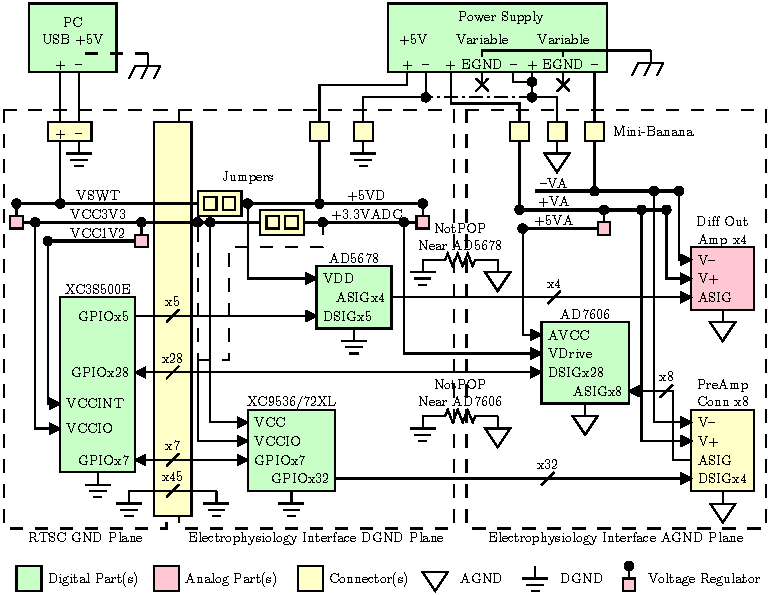
\includegraphics{./figures/Ground} 
	\caption{Ground planes\label{fig:Ground}}
\end{figure}

The communication between parts powered by the analog and digital supplies requires that the signals be referenced to a common node.  Thus, the analog and digital grounds are connected near the bench-top power supply.  This has the effect of minimizing ground-bounce by directing the current return of most of the fast switching digital signals through the digital power supply lead, but it directs the signal return current, from signals that cross the ground planes, to the bench-top power supply before it can return to the signal source, yielding a large signal loop that increases radiated emissions~\cite{Montrose1999}.

Both the AD5678 and AD7606 recommend that, if analog and digital ground connection is needed, it should be close to the the respective IC~\cite{AD7606ds,AD5678ds}.  Near the AD5678 and near the AD7606, pads for $0\unit{\Omega}$ resistors may be populated to allow a shorter signal current return path, but if multiple signals switch at once, the actual non-zero resistance of the resistor, via, and trace connecting the ground planes will be out of balance with the signal trace resistance and may allow signal return current in the ground planes to divert back to the bench-top power supply.

Future designs should consider suggestions in~\cite{Montrose1999} for completely isolating analog and digital power and ground using opto-isolators or isolation transformers for digital signals that need to communicate between analog and digital circuits, or an alternative is to bridge analog and digital planes under signals that interface with analog and digital circuits.


\subsubsection{Decoupling Capacitors}

Capacitors are populated on the RTSC board and the Electrophysiology Interface board for the purpose of maintaining quality power supply voltages in the presence of high switching currents and radiated and conducted electromagnetic interference (EMI).  Capacitors connected to the power and ground planes perform three functions: decoupling which provides a source of DC power near components that meets demand for short duration power surges and keeping RF energy generated by components from propagating into the power supply network, bypassing which provides a low impedance path to ground for high frequency noise that may interfere with components, and bulk capacitance that is used to maintain a constant DC voltage for situations that cause a large $\mathrm{d}i/\mathrm{d}t$, such as all digital signals switching simultaneously~\cite{Montrose1999}.

Ideal capacitors with large capacitance values yield a low impedance at high frequencies and store more energy than low capacitance values, but the electrolytic and tantalum constructions that allow large capacitance values in small volumes have comparatively large equivalent series resistance (ESR) and equivalent series inductance (ESL) that limit their usefulness at higher frequencies and for large $\mathrm{d}i/\mathrm{d}t$.  Thus low ESR, ESL, and value ceramic capacitors are often used in parallel with electrolytic or tantalum capacitors to provide the required capacitance for decoupling and bypassing~\cite{Montrose1999}.  The capacitors are also placed as close as possible to the component that needs bypassing and decoupling to limit the added inductance in the length of PCB trace between the capacitor and the component.  Because of resonance effects with parallel capacitors, their values should be separated by at least two orders of magnitude (i.e. the value of the electrolytic capacitor should be at least 100 times greater than the value of the ceramic capacitor)~\cite{Montrose1999}.  Power and ground planes, themselves being two parallel plates, also act as capacitors with the advantage of having effectively no ESR and very low ESL and may provide sufficient capacitance, with closely spaced planes for slow switching frequency and slew rate circuits, but the planes should be spaced by less than $0.1\unit{in}$ and vias limit the effective capacitance of the parallel planes~\cite{Montrose1999}.

On the Electrophysiology Interface board, a capacitor that performs decoupling and bypass functions is populated for each power supply pin of a component and each power pin of a connector, and the capacitor is placed as close as possible to the pin.  One $0.1\unit{\mu F}$ ceramic capacitor is used, if no recommendation is given by the part's data sheet.  The AD5678 data sheet recommends a $10\unit{\mu F}$ capacitor in parallel with a low ESR $0.1\unit{\mu F}$ capacitor~\cite{AD5678ds}.  If a surface mount ceramic capacitor is available with the recommended capacitance, a ceramic capacitor is used even if the data sheet suggests using a tantalum or electrolytic capacitor.  One large value electrolytic capacitor is available for each of the +5VD, +VA, and $\unit{-VA}$ power supplies to provide bulk capacitance.

	
\subsection{Programmable Logic Configuration}

%Description of configuration flash ROM for storing FPGA configuration data and configuring FPGA without a PC
The Xilinx\textsuperscript{\textregistered} XC3S500E FPGA is a volatile programmable logic device, meaning that the configuration of the FPGA is lost when power is removed.  The Xilinx\textsuperscript{\textregistered} XC9536/72XL CPLD is a non-volatile programmable logic device.  Configuration files that describes the state of the FPGA and CPLD are produced by the Xilinx\textsuperscript{\textregistered} ISE Design Suite.  A mechanism must be in place to load the configuration into the FPGA after every power cycle.  The CPLD configuration only needs to be loaded once; it will retain its configuration between power cycles.

Two configurations options are available on the RTSC to load a configuration to the FPGA.  A jumper selects whether the FPGA will be configured using the Joint Test Action Group (JTAG) interface or the Xilinx\textsuperscript{\textregistered} XCF00S  Platform Flash EEPROM.  The connections between the FPGA and the Platform Flash and the jumper options are shown in Figure~\ref{fig:Config}.

\begin{figure}[H]
	\centering 
		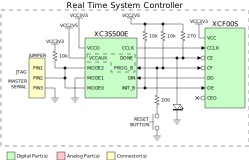
\includegraphics{./figures/Config} 
	\caption{Connection of the Platform FLASH Configuration PROM to the FPGA~\cite{DigilentNexys2rm,DigilentNexys2sch}\label{fig:Config}}
\end{figure}

There are three pins on the FPGA that control the configuration mode.  These pins are labeled MODE[0:2].  The FPGA is capable of several configuration modes, but the modes available on the RTSC are shown in Table~\ref{tab:ConfigMode}.

\renewcommand{\arraystretch}{1.3}
\begin{table}[h]
\centering
\begin{tabular}{|l|l|}
\hline
MODE[0:2]& Configuration mode\\
\hline
[0 0 0] & Master Serial (Platform Flash)\\
\hline
[1 0 1] & JTAG Mode\\
\hline
\end{tabular}
\caption{FPGA configuration modes from a table in~\cite{Spartan3ConfigUG}\label{tab:ConfigMode} }

\end{table}
\renewcommand{\arraystretch}{1.0}

\subsubsection{Master Serial}

Xilinx\textsuperscript{\textregistered}  has created a line of flash ICs that make on board configuration very simple.  Using the Platform Flash ICs, the Spartan 3E FPGA can configure itself in Master Serial mode where the FPGA controls the serial data clock and enables the flash chip~\cite{Spartan3ConfigUG}.  The XCF04S 4Mbit Platform Flash device provides enough storage for one configuration file for the XC3S500E~\cite{Spartan3ConfigUG}.

Upon power up, the INIT\textunderscore B and DONE open-drain IO pins and the PROG\textunderscore B input pin are pulled high.  INIT\textunderscore B going high causes the FPGA to sample the MODE[0:2] pins, and if Master Serial is the mode selected, INIT\textunderscore B is pulled low, resetting the Platform Flash while the configuration is cleared, after which INIT\textunderscore B is allowed to go high.  DONE is pulled low, enabling the Platform Flash, and the FPGA begins to generate a clock on CCLK, causing the Platform Flash to present data on its DO pin.  After configuration is complete, DONE is allowed to go high, and by virtue of the resistor and LED connected to the pin, the LED will turn on and DONE and $\overline{\mathrm{CE}}$ voltage will be at $\unit{V} _ {\unit{F}}$ of the LED~\cite{Spartan3ConfigUG}.

Pulsing PROG\textunderscore B low for at least $500\unit{ns}$ will cause the FPGA to clear the configuration memory, pull INIT\textunderscore B low, and sample the MODE[0:2] pins when INIT\textunderscore B goes high~\cite{Spartan3ConfigUG}.  The reset button on the RTSC will cause the FPGA to clear its configuration and reconfigure itself or wait for the JTAG interface, depending on the status the MODE[0:2] pins.


\subsubsection{JTAG}

A method of testing interconnects between integrated circuits (IC) on a PCB called Boundary Scan is commonly implemented on digital ICs.  The Boundary Scan standard was developed by the Joint Test Action Group (JTAG) and later adopted as an IEEE standard with the designation IEEE Std. 1149.1.  Boundary Scan, which is commonly referred to as JTAG~\cite{CorelisJTAG}.

The JTAG interface also provides in-circuit programming capabilities which is the feature that is used to configure the FPGA, Platform Flash, and CPLD.  Multiple devices can be daisy-chained in a single JTAG interface.  The list of signals is in the Table~\ref{tab:JTAGSigName}, which is based on~\cite{CorelisJTAG}.




%
% Table begins
% 


\renewcommand{\arraystretch}{1.3}
\begin{table}[h]
\centering
\begin{tabular}{|l|l|p{3in}|}
\hline

Abbreviation&

Signal&

Description\\
\hline

TCK&

Test Clock&

Clock signal bussed to all devices in the chain\\
\hline


TMS&

Test Mode Select&

Mode signal bussed to all devices in the chain\\
\hline


TDI&

Test Data In&

Data to be shifted into device JTAG logic from the previous device in the chain.  Sampled on rising edge of TCK\\
\hline


TDO&

Test Data Out&

Data to be shifted out of device JTAG logic to the next device in the chain.  Updated on falling edge of TCK\\
\hline
\end{tabular}
\caption{JTAG signal names and descriptions~\cite{CorelisJTAG}\label{tab:JTAGSigName} }
\end{table}
\renewcommand{\arraystretch}{1.0}

To program the FPGA, Platform Flash, or CPLD, a JTAG programming cable available from Digilent\textsuperscript{\textregistered}, Xilinx\textsuperscript{\textregistered}, or another vendor may be connected to the JTAG header, or the JTAG capabilities of the Cypress microcontroller may be utilized with the Digilent\textsuperscript{\textregistered} ADEPT PC software.  Details of the JTAG connections, which are based on~\cite{DigilentNexys2sch}, are shown in Figure~\ref{fig:JTAGChain}.  The resistors on the TCK, TMS, and XC3S500E TDI lines are required to be $>68\unit{\Omega}$ for $3.3\unit{V}$ JTAG interfaces ($0\unit{\Omega}$ for $2.5\unit{V}$ interface)~\cite{Spartan3ConfigUG}.  Reference~\cite{DigilentNexys2sch} uses $200\unit{\Omega}$ resistors.

\begin{figure}[H]
	\centering 
		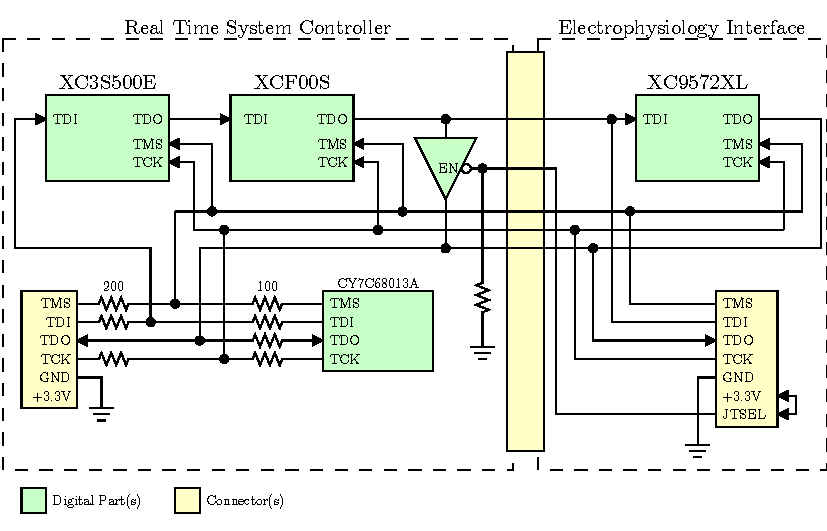
\includegraphics{./figures/JTAGChain} 
	\caption{Signals in the JTAG scan chain; RTSC connections based on~\cite{DigilentNexys2sch}\label{fig:JTAGChain}}
\end{figure}

The RTSC routes the JTAG scan chain through the FPGA, then the Platform Flash, and finally over the Hirose FX2 connector.  If a peripheral board connected to the FX2 connector does not connect to the RTSC's JTAG scan chain, a tri-state buffer, with its active-low output-enable pin pulled low, routes the TDO signal of the Platform Flash to the Cypress microcontroller and JTAG programming cable header.  To enable the CPLD on the Electrophysiology Interface board to be programmed through the JTAG scan chain of the RTSC, the TDO signal from the Platform Flash is routed to the TDI pin of the CPLD, the TDO pin of the CPLD is routed to the Cypress microcontroller and JTAG programming header on the RTSC, and the TMS and TCK signals are bussed to the CPLD.  A header on the Electrophysiology Interface board allows probing of the JTAG signals, or if the board is not connected to the RTSC, a JTAG programming cable may be connected to the header to program the CPLD.  The output-enable pin of the tri-state buffer is routed to the JTSEL signal on the Electrophysiology Interface board.  To prevent the tri-state buffer and CPLD from acting as an output on the same signal, connecting JTSEL to $+3.3\unit{V}$ on the header on the Electrophysiology Interface board will disable the output of the tri-state buffer.  Thus, simply connecting the Electrophysiology Interface board to the RTSC board will put the CPLD in the RTSC's JTAG scan chain.

Steps for configuring the FPGA or CPLD or loading a configuration file into the Platform Flash in JTAG mode:

\begin{enumerate}
	\item Set the configuration jumper on the RTSC to JTAG Mode

	\item If the Electrophysiology Interface board is connected to the RTSC, configure the power supplies so that the CPLD's VCC and VCCIO pins will be powered

	\item Connect the USB cable to the RTSC, or connect the JTAG programming cable to the JTAG header on the RTSC

	\item Turn on power to the RTSC and Electrophysiology Interface, if it's connected

	\item Follow the steps required in the PC software for the programming cable to load the configuration file onto the FPGA, Platform Flash, or CPLD
\end{enumerate}


\subsection{Real Time System Controller Board Circuit Design}

This sections describes the relevant circuitry on the Digilent\textsuperscript{\textregistered} Nexys\textsuperscript{TM} 2 FPGA development board that is utilized by the Data Acquisition and Stimulation System (DASS) as the Real Time System Controller (RTSC) Board.  Replacing the Nexys\textsuperscript{TM} 2 FPGA development board with a custom RTSC Board or designing a system based on the DASS with more channels, as described in section~\ref{sec:scaling}, would require the duplication of the following circuitry or the design of new circuitry that would preform similar functions.

\subsubsection{Cypress Microcontroller}

%Description of the data connections between the FPGA and Cypress Microcontroller and the USB connection to the PC
The Cypress CY7C68013C EZ-USB\textsuperscript{\textregistered} microcontroller on the RTSC provides a USB interface to the FPGA and provides JTAG programming capabilities without the need for separate JTAG programming hardware~\cite{DigilentNexys2rm}.  Unlike a general purpose microcontroller or FPGA, the Cypress microcontroller can connect directly to the USB signal lines with its integrated USB transceiver~\cite{CypressDS}.  Figure~\ref{fig:Cypress} shows the connections between the Cypress microcontroller and the FPGA on the RTSC.

%Table: USB Connector

%5V power supplied by the USB host at up to 500mA
%D+	Bidirectional asynchronous differential twisted pair serial data
%D-
%GND signal and power return

%The Cypress microcontroller acts a slave on the USB bus.  When the Nexys2 is connected to a PC, the Cypress microcontroller pulls the (check) high to signal the host that it is on the bus.

\begin{figure}[H]
	\centering 
		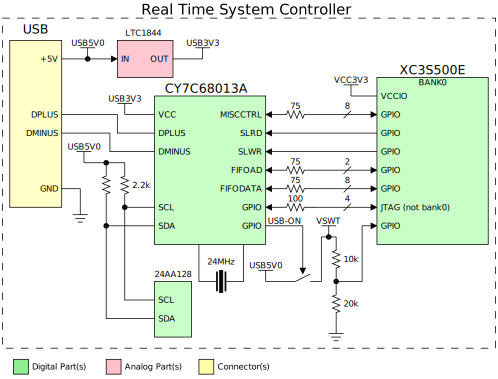
\includegraphics{./figures/Cypress} 
	\caption{Connections for the USB interface on the RTSC board~\cite{DigilentNexys2rm,DigilentNexys2sch}\label{fig:Cypress}}
\end{figure}

A USB peripheral must not draw more than 100mA from the host until it has negotiated the full power capabilities of the bus.  The Cypress microcontroller receives 3.3V power from a regulator connected directly to the 5V USB supply. The rest of the RTSC board can be powered from the USB supply, but if the entire RTSC board is to be powered by the USB supply voltage, it must not power all of its circuits immediately upon connection because the board would draw more than 100mA~\cite{DigilentNexys2rm}.  When the Cypress microcontroller has negotiated the full power capabilities of the bus, the USB-ON signal, which is connected to the gate of a NMOS transistor, is toggled connecting the USB5V0 voltage to the rest of the board~\cite{DigilentNexys2rm}.

Connections between the Cypress microcontroller have series resistors where the Cypress microcontroller signal can be an output.  This is to limit the current in the case of the FPGA pin being setup as an output simultaneously with the Cypress microcontroller.

Data transfer from the FPGA to the USB host is facilitated by a first in, first out (FIFO) buffer in the Cypress microcontroller.  A FIFO acts as a dual port memory allowing a device to push data into the memory; the FIFO will keep track of the memory address to be written.  The same device or a second device can then read from the memory and the FIFO will fetch the oldest data in memory that has yet to be read.  In this way, two devices, operating on different clocks or with other tasks to complete, can share data without being synchronized, or one device can store a stream of data and retrieve the data stream in the order written without the need for memory addressing logic.

Eight of the data connections between the Cypress microcontroller and the FPGA carry the FIFO data that can be written or read by the FPGA (FIFODATA).  The Cypress microcontroller internally reads or writes to the other side of the FIFO with data to or from the USB bus~\cite{CypressDS}.  A 24MHz crystal provides a dedicated clock to the Cypress microcontroller.  A 12pF capacitor is required from each terminal of the crystal to ground to stabilize the oscillation~\cite{DigilentNexys2rm}.  A 24AA128 EEPROM, that contains the Digilent\textsuperscript{\textregistered} firmware, is connected to the I$^2$C pins of the Cypress microcontroller, which are open-drain outputs and hysteresis inputs that must be pulled up to 3.3V even if unconnected~\cite{CypressDS}; although, the RTSC pulls these signals to USB5V0~\cite{DigilentNexys2sch}.


\subsubsection{RS232 Control Interface}

%Description of RS232 level shifter that allows the FPGA to interface with the PC over RS232
Control signals can be communicated separately from the USB interface using the serial port on the RTSC.  PC serial ports conform to the RS232 standard which uses signaling voltages that are incompatible with the 3.3VTTL/CMOS logic of the FPGA~\cite{StrangioRS232}.  The ST232 level shifting IC converts logic LOW and HIGH of LVTTL/CMOS voltages to RS232 compatible voltages without the need for higher voltage supplies~\cite{ST232ds}.  Table~\ref{tab:RS232TTL} shows the logic voltage levels compatible with the Xilinx\textsuperscript{\textregistered} XC3S500E FPGA IO pins configured for LVTTL and logic voltages compatible with the RS232 standard~\cite{Spartan3eDS,StrangioRS232}.

\renewcommand{\arraystretch}{1.3}
\begin{table}[h]
\centering 
  \begin{tabular}{| l | c | c | c | c |}
    \hline
    Logic & LOW$_{\mathrm{min}}$ & LOW$_{\mathrm{max}}$ & HIGH$_{\mathrm{min}}$ & HIGH$_{\mathrm{max}}$ \\
	\hline
    LVTTL & $-0.5\unit{V}$ & $+0.8\unit{V}$ & $+2.0\unit{V}$ & $+3.8\unit{V}$ \\
	\hline
    RS232 & $+3.0\unit{V}$ & $+25.0\unit{V}$ & $-25.0\unit{V}$  & $-3.0\unit{V}$ \\
    \hline
  \end{tabular}
  \caption{FPGA and RS232 logic voltage level comparison\label{tab:RS232TTL} }

\end{table}
\renewcommand{\arraystretch}{1.0}

RS232 communication is asynchronous and full duplex with separate receive (often labeled as RX or R) and transmit (often labeled as TX or T) data lines and without a dedicated clock signal.  The signals other than RX and TX are not necessary for simple communication between one host and peripheral~\cite{StrangioRS232}.

As shown in Figure~\ref{fig:RS232}, the ST232 level shifting IC is between the FPGA's GPIO pins being used for RX and TX signals that can be connected to a PC via the standard pinout D-Subminiature 9 pin (DB9) connector.  The ST232 is capable of passing two separate RS232 communication busses (R1/T1 IN/OUT and R2/T2 IN/OUT), but only one set is used by the FPGA.

\begin{figure}[H]
	\centering 
		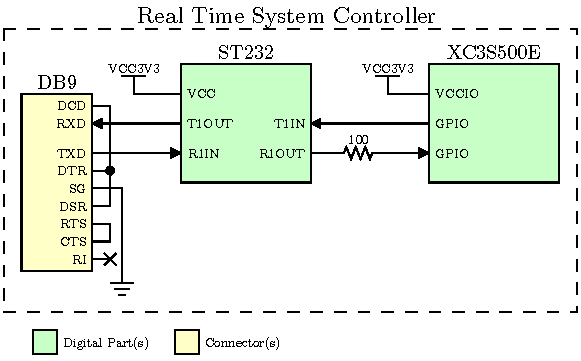
\includegraphics{./figures/RS232} 
	\caption{RS232 level shifter that allows a PC serial port to communicate with the FPGA~\cite{DigilentNexys2rm,DigilentNexys2sch}\label{fig:RS232}}
\end{figure}

For a future design, an alternative to provide PC communication is to use an TTL-232RG cable from FTDI that connects to a USB port and provides a virtual serial port to the PC while providing a TTL serial UART compatible interface to connect to the FPGA, directly~\cite{FTDIUSBSerial}.

%A series resistor is placed between the FPGA's RX GPIO pin and the R1OUT of the ST232  to limit current into an unpowered Nexys2 if a PC or other device is connected to the DB9.




\subsubsection{DRAM}

%Description of DRAM connections to the FPGA
The RTSC board contains a 54-pin, ball grid array (BGA) packaged MT45W8MW16BGX 128Mbit DRAM IC from Micron\textsuperscript{\textregistered} with its address and data bus connected in parallel with a JS28F128 128Mb Flash ROM fron Intel\textsuperscript{\textregistered}~\cite{DigilentNexys2rm}.  The DRAM is used by the configuration on the FPGA to store stimulation waveform data, and the Flash ROM is not used~\cite{BatzerMSEE}.  Figure~\ref{fig:dram} shows the connections between the Xilinx\textsuperscript{\textregistered} XC3S500E FPGA and the DRAM and Flash ROM on the RTSC board.

\begin{figure}[htb]
	\begin{singlespace}
	\centering	
		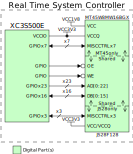
\includegraphics{./figures/DRAM} 
	\caption{Connections between the FPGA and the DRAM and Flash memory ICs on the RTSC board~\cite{DigilentNexys2rm,DigilentNexys2sch}\label{fig:dram}}
	\end{singlespace}
\end{figure}

The DRAM requires a $+1.8\unit{V}$ power supply for its internal circuitry and has a dedicated supply pin for interface logic as described in section~\ref{sec:rtscpower}.  Seven control signals are connected exclusively between the FPGA and DRAM IC.  The 23-bit wide address bus, 16-bit bi-directional data bus, output enable ($\overline{\mathrm{OE}}$) signal, and write enable ($\overline{\mathrm{WE}}$) signal are connected to both the DRAM and Flash IC.  The Flash IC has a 25-bit address bus, but its MSbit and LSbit are pulled LOW~\cite{DigilentNexys2sch}.  Three control signals are connected exclusively between the FPGA and Flash ROM IC.

\subsection{Electrophysiology Interface Board Circuit Design}

This section describes and documents the design of the custom circuitry on the Electrophysiology Interface Board.  These circuits were implemented on a custom printed circuit board (PCB), described in section~\ref{sec:build}.  The circuit designs in this section could also be used in the creation of a 64 channel system, as proposed in section~\ref{sec:scaling}, for use in microelectrode array (MEA) electrophysiology experiments.

\subsubsection{Digital to Analog Converter}\label{sec:dac}

%Description of DAC connections to the FPGA
The Analog Devices AD5678-2 was chosen to be the DAC on the Electrophysiology Interface board because of previous experience with the device in the Neurobiology Engineering Laboratory~\cite{BatzerCorsiCrampton}.  The design for the circuit shown in Figure~\ref{fig:DAC} is based on a breadboarded prototype circuit~\cite{BatzerCorsiCrampton} and recommendations in the device data sheet~\cite{AD5678ds}.

\begin{figure}[H]
	\centering 
		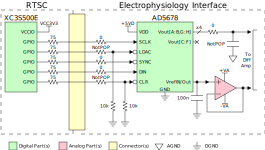
\includegraphics{./figures/StimAmp} 
	\caption{FPGA connections to the DAC\label{fig:DAC}}
\end{figure}

Signals from the Xilinx\textsuperscript{\textregistered} XC3S500E FPGA on the RTSC board are routed through the Hirose FX2 connector to the Electrophysiology Interface board and the 40-pin test header, finally going through a $0\unit{\Omega}$ resistor before being routed to the digital control pins of the AD5678.  The four 16-bit DAC analog outputs are routed to the Differential Output Amplifier circuits through a resistor that may be used, in concert with a capacitor, to implement an RC-type low pass filter.  The four 12-bit DAC outputs are left unconnected.  The FPGA configures the AD5678 to use its internal voltage reference for DAC operations, and thus, the Vref pin acts as the output of the internal voltage reference.  A 100nF capacitor is placed between the Vref pin and ground to stabilize the reference output~\cite{AD5678ds}, and the reference output voltage is used in the Differential Output Amplifier circuit, which requires the use of a buffer amplifier~\cite{AD5678ds}.  A description of each digital control pin is in Table~\ref{tab:AD5678Pins}.

\renewcommand{\arraystretch}{1.3}
\begin{table}[h]
\centering
\begin{tabular}{|l|p{4in}|}
\hline
Pin	& Function\\
\hline
$\overline{\mathrm{SYNC}}$	& Active low synchronization signal for input data, similar to SPI CS\\
\hline
DIN	& Serial data input\\
\hline
SCLK	& Serial clock input\\
\hline
$\overline{\mathrm{LDAC}}$	& Updates outputs simultaneously on a low pulse, it may be tied low if unused\\
\hline
$\overline{\mathrm{CLR}}$	& Falling edge triggered clear input that can set all the outputs to zero, mid-scale, or full-scale (default zero), pull down resistor keeps this from being noise triggered if unused\\
\hline
\end{tabular}
\caption{AD5678 Digital Pin Functions~\cite{AD5678ds}\label{tab:AD5678Pins} }

\end{table}
\renewcommand{\arraystretch}{1.0}

$\overline{\mathrm{SYNC}}$, DIN, and SCLK are mandatory signals for executing commands and loading data into the DAC.  The signals are compatible with SPI\textsuperscript{\textregistered}, QSPI\textsuperscript{TM}, MICROWIRE\textsuperscript{TM}, and DSP interface standards~\cite{AD5678ds}.  The $\overline{\mathrm{LDAC}}$ and $\overline{\mathrm{CLR}}$ signals provide additional functionality that is not used in the current version of the FPGA configuration.  Thus, the $0\unit{\Omega}$ resistors are not populated on the Electrophysiology Interface board, allowing the FPGA's GPIO pins to be accessed at the test header and used for other purposes if needed, and the DAC pins are pulled to ground through $10\unit{k\Omega}$ resistors to keep the inputs at a known state that will not affect the operation of the DAC.

The AD5678 contains a power-on reset circuit that sets the DAC outputs to 0V upon power up, which due to the Differential Output Amplifier may yield a significant voltage across the stimulation electrodes, which may be incompatible with the biological setup~\cite{AD5678ds}.  Therefore, upon power-up, the FPGA should immediately write DAC outputs or set the Clear Code Register and pulse the $\overline{\mathrm{CLR}}$ signal to set the DAC outputs to a value that will yield a voltage across the stimulation electrodes that is compatible with the experimental setup.  $\overline{\mathrm{CLR}}$ is a falling edge triggered signal that can also be used to asynchronously set all of the outputs to the state defined in the Clear Code Register of the AD5678~\cite{AD5678ds}.


\subsubsection{Differential Output Amplifier}\label{sec:DOA}

%Design and description of the differential output amplifier providing gain and offset to DAC output including SPICE simulations
The analog output of the AD5678-2, when using the internal $2.5\unit{V}$ voltage reference, can vary over the range of $0\unit{V}$ to $5\unit{V}$.  The output voltage is given by the equation
\begin{equation}
\label{equ:DACout}
\mathrm{Vout} = 2 \times \mathrm{VrefOut}  \times \frac{D}{2^N},
\end{equation}
where $D$ is the decimal equivalent of the binary value loaded into the DAC output register and $N$ is the resolution of the DAC (16 for the DAC outputs used on the Electrophysiology Interface board)~\cite{AD5678ds}.  It is desirable to have pulses as high as $10\unit{V}$ and with biphasic shapes to perform some electrophysiology experiments~\cite{Olivo,Kladt2010}.  Thus, some form of signal gain and offset is needed to extend the range of the output signal.  It is also desirable to be able to perform experiments with differential outputs, so the single-ended output of the DAC is converted to a differential output.

The design of Differential Output Amplifier circuit as shown in Figure~\ref{fig:DiffAmp} consists of a difference amplifier circuit, implemented with operational amplifier (op-amp) OA1, to perform the gain and offset operations on the DAC output and an inverting amplifier, implemented with op-amp OA2, to create a differential output.  The Differential Output Amplifier design is replicated for each of the DAC outputs to create four unique outputs that can be connected to stimulation electrodes single-endedly (between Vout+ and AGND or $\mathrm{Vout-}$ and AGND) or differentially (between Vout+ and $\mathrm{Vout-}$).

\begin{figure}[H]
	\centering 
		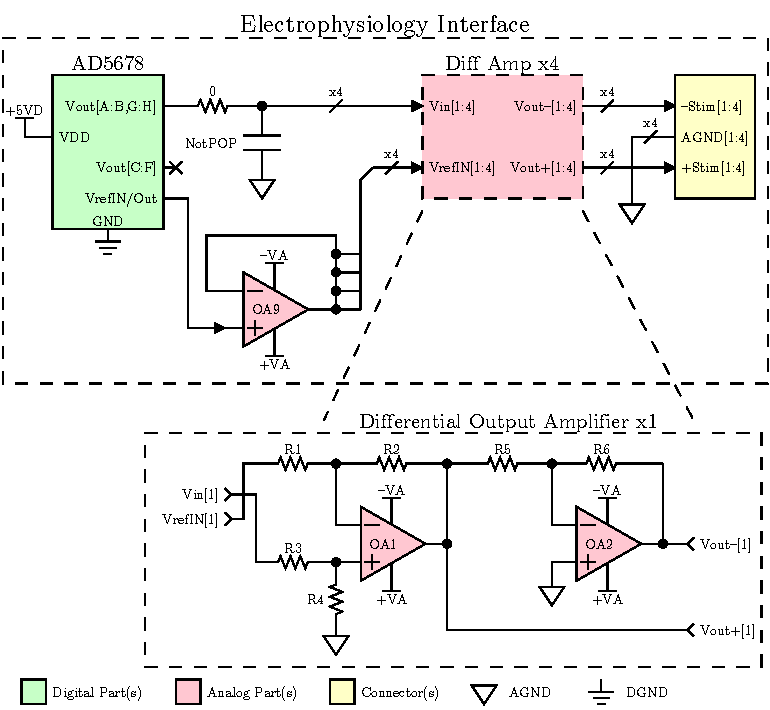
\includegraphics{./figures/DiffAmp} 
	\caption{Differential Output Amplifier\label{fig:DiffAmp}}
\end{figure}

The difference amplifier op-amp configuration is well known, with its operation described by equation
\begin{equation}
\label{equ:DifferenceAmp1}
\mathrm{Vout+} = \frac{R_2}{R_1} \frac{1 + R_1/R_2}{1 + R_3/R_4} \mathrm{Vin} - \frac{R_2}{R_1} \mathrm{VrefIN};
\end{equation}
choosing resistor values with the constraint
\begin{equation}
\label{equ:DifferenceAmp2}
\frac{R_1}{R_2}  = \frac{R_3}{R_4} 
\end{equation}
yields the simpler form
\begin{equation}
\label{equ:DifferenceAmp3}
\mathrm{Vout+} = \frac{R_2}{R_1} (\mathrm{Vin} - \mathrm{VrefIN}),
\end{equation}
which has the gain and offset elements needed to fulfill the design requirements~\cite{AlexanderSadiku2004}.

The $0\unit{V}$ to $5\unit{V}$ range of the DAC outputs can be made symmetrical around $0\unit{V}$ by subtracting $2.5\unit{V}$, yielding a range of $-2.5\unit{V}$ to $2.5\unit{V}$.  Thus, the range of Vout+ is $-2.5\unit{V}  \times R_2/R_1$ to $2.5\unit{V} \times R_2/R_1$, allowing the output range to be easily calculated and changed if needed.  Since the AD5678 makes its internal $2.5\unit{V}$ voltage reference accessible on an external pin, using that voltage as an input to the difference amplifier eliminates the need for an external voltage reference circuit that would involve a resistor network susceptible to inaccuracies in the power supply voltage or a specialized voltage reference IC.  Substituting the midscale DAC code 0x7FFF into equation~\eqref{equ:DACout} and~\eqref{equ:DifferenceAmp3} yields $\mathrm{Vout+}=76 \unit{\mu V} \times R_2/R_1$ which is very close to $0\unit{V}$.  Programming the AD5678 to output midscale codes on the DAC outputs after power-on reset will ensure than stimulation electrodes have a low DC voltage without having to write the DAC code at every power cycle.

An inverted output is needed to implement a differential output amplifier.  This can be accomplished with an op-amp in an inverting configuration.  The equation for the inverting amplifier is \begin{equation}
\label{equ:InvertingAmp1}
\mathrm{Vout-} = -\frac{R_6}{R_5} \mathrm{Vout+} ;
\end{equation}
choosing $R_5 = R_6$ will make $\mathrm{Vout-}$ the inverse of Vout+~\cite{AlexanderSadiku2004}.  The ratio $R_2/R_1$ is set to $3$ to produce single-ended output range of $-2.5\unit{V}  \times R_2/R_1$ to $2.5\unit{V} \times R_2/R_1  \Rightarrow -7.5\unit{V}$ to $7.5\unit{V}$, which will be close to the saturation voltages of an op-amp powered from $\pm 9\unit{V}$ supplies.  Table~\ref{tab:DiffOutAmpRes} shows resistor values chosen and calculated for the design.

\renewcommand{\arraystretch}{1.3}
\begin{table}[h]
\centering 
\begin{tabular}{l l l l}
\hline
Choose	& $R_1$	& $R_3$ & $R_2/R_1$	\\
	&	$1\unit{k\Omega}$	&  $1\unit{k\Omega}$ &	$3$	\\
Yields	& $R_2$ &  $R_4$ &	\\
	&	$3\unit{k\Omega}$	& $3\unit{k\Omega}$ &	\\
\hline
Choose	& $R_5$ &	&	\\
	&	$1\unit{k\Omega}$	& 	&	\\
Yields	& $R_6$ &  & 	\\
	&	$1\unit{k\Omega}$	&	&	\\
\hline
\end{tabular}
\caption{Resistor values for the Differential Output Amplifier\label{tab:DiffOutAmpRes} }

\end{table}
\renewcommand{\arraystretch}{1.0}

The dual packaged LT1124-1 precision op-amp from Linear Technology\textsuperscript{\textregistered} was chosen because the LT1124/LT1125 part family was used in~\cite{StahlMSEE,BatzerCorsiCrampton}, SPICE amplifier models are available for LTspice\textsuperscript{\textregistered} circuit simulation software, the dual package allows the Differential Output Amplifier block with two op-amps to be implemented with only one IC, and the -1 option specifies a standard pinout 8-SO surface mount part so other op-amp models may be tested with the design~\cite{LT11245ds}.

According to~\cite{AD5678ds}, the voltage reference output should be buffered if used to drive a load, so a single op-amp in a voltage follower configuration is used to buffer the reference voltage to the Differential Output Amplifier blocks.  One half of an LT1124-1 is used to be consistent with the other op-amps on the Electrophysiology Interface board.  The buffer op-amp, OA9, drives current through $R_1$ of the Differential Output Amplifier block; thus, the op-amp will need to be capable of driving current to four amplifier blocks.  The maximum current the OA9 will need to provide will be determined by the maximum voltage across $R_1$ multiplied by four.  The maximum voltage across $R_1$ will be when Vin equals $0\unit{V}$, which would yield a maximum current of $(\mathrm{Vref}-0\unit{V})/R_1\times4=2.5\unit{V}/1\unit{k\Omega} \times4=10\unit{mA}$.  It may be necessary to choose higher value resistors if the buffer is needed to drive more amplifier blocks or it is seen that the output voltage of OA9 changes during use.

The design of the Differential Output Amplifier was entered into the circuit simulation program LTspice\textsuperscript{\textregistered}, as shown in Figure~\ref{fig:DiffAmp}, to test the design of the circuit.  The first test performed was a DC sweep of Vin to display the transfer function from the outputs Vout+ and $\mathrm{Vout-}$.  The transfer function is shown in Figure~\ref{fig:DCSweep}.  Saturation occurs at $40\unit{mV}$ and $4.95\unit{V}$ yielding saturation voltages of approximately $\pm7.4\unit{V}$, allowing for almost the entire range of DAC output to be in the linear region and yielding a maximum possible output voltage, if taken differentially, of $14.8\unit{V}$.

\begin{figure}[H]
	\centering 
		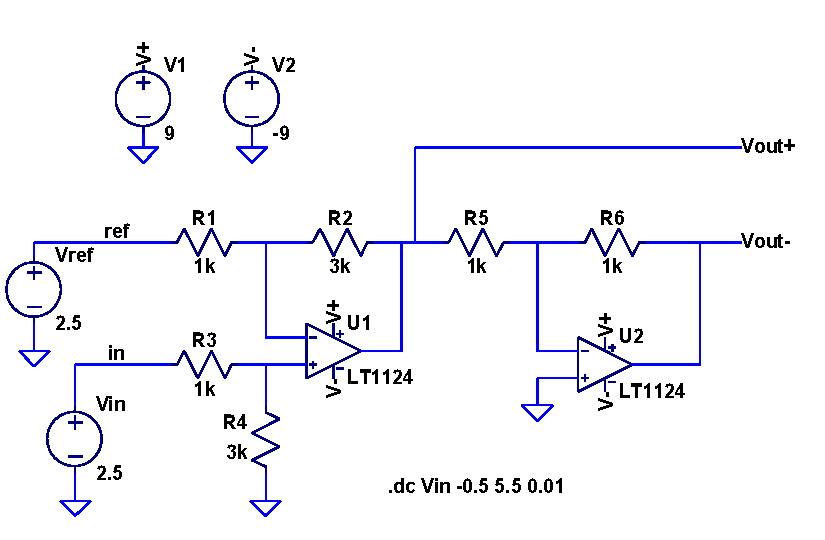
\includegraphics{./figures/LTSchem} 
	\caption{LTspice\textsuperscript{\textregistered} schematic of the Differential Output Amplifier circuit\label{fig:DiffAmp}}
\end{figure}

\begin{figure}[H]
	\centering 
		\resizebox{\textwidth-0.5in}{!}{% GNUPLOT: LaTeX picture with Postscript
\begingroup
  \makeatletter
  \providecommand\color[2][]{%
    \GenericError{(gnuplot) \space\space\space\@spaces}{%
      Package color not loaded in conjunction with
      terminal option `colourtext'%
    }{See the gnuplot documentation for explanation.%
    }{Either use 'blacktext' in gnuplot or load the package
      color.sty in LaTeX.}%
    \renewcommand\color[2][]{}%
  }%
  \providecommand\includegraphics[2][]{%
    \GenericError{(gnuplot) \space\space\space\@spaces}{%
      Package graphicx or graphics not loaded%
    }{See the gnuplot documentation for explanation.%
    }{The gnuplot epslatex terminal needs graphicx.sty or graphics.sty.}%
    \renewcommand\includegraphics[2][]{}%
  }%
  \providecommand\rotatebox[2]{#2}%
  \@ifundefined{ifGPcolor}{%
    \newif\ifGPcolor
    \GPcolorfalse
  }{}%
  \@ifundefined{ifGPblacktext}{%
    \newif\ifGPblacktext
    \GPblacktexttrue
  }{}%
  % define a \g@addto@macro without @ in the name:
  \let\gplgaddtomacro\g@addto@macro
  % define empty templates for all commands taking text:
  \gdef\gplbacktext{}%
  \gdef\gplfronttext{}%
  \makeatother
  \ifGPblacktext
    % no textcolor at all
    \def\colorrgb#1{}%
    \def\colorgray#1{}%
  \else
    % gray or color?
    \ifGPcolor
      \def\colorrgb#1{\color[rgb]{#1}}%
      \def\colorgray#1{\color[gray]{#1}}%
      \expandafter\def\csname LTw\endcsname{\color{white}}%
      \expandafter\def\csname LTb\endcsname{\color{black}}%
      \expandafter\def\csname LTa\endcsname{\color{black}}%
      \expandafter\def\csname LT0\endcsname{\color[rgb]{1,0,0}}%
      \expandafter\def\csname LT1\endcsname{\color[rgb]{0,1,0}}%
      \expandafter\def\csname LT2\endcsname{\color[rgb]{0,0,1}}%
      \expandafter\def\csname LT3\endcsname{\color[rgb]{1,0,1}}%
      \expandafter\def\csname LT4\endcsname{\color[rgb]{0,1,1}}%
      \expandafter\def\csname LT5\endcsname{\color[rgb]{1,1,0}}%
      \expandafter\def\csname LT6\endcsname{\color[rgb]{0,0,0}}%
      \expandafter\def\csname LT7\endcsname{\color[rgb]{1,0.3,0}}%
      \expandafter\def\csname LT8\endcsname{\color[rgb]{0.5,0.5,0.5}}%
    \else
      % gray
      \def\colorrgb#1{\color{black}}%
      \def\colorgray#1{\color[gray]{#1}}%
      \expandafter\def\csname LTw\endcsname{\color{white}}%
      \expandafter\def\csname LTb\endcsname{\color{black}}%
      \expandafter\def\csname LTa\endcsname{\color{black}}%
      \expandafter\def\csname LT0\endcsname{\color{black}}%
      \expandafter\def\csname LT1\endcsname{\color{black}}%
      \expandafter\def\csname LT2\endcsname{\color{black}}%
      \expandafter\def\csname LT3\endcsname{\color{black}}%
      \expandafter\def\csname LT4\endcsname{\color{black}}%
      \expandafter\def\csname LT5\endcsname{\color{black}}%
      \expandafter\def\csname LT6\endcsname{\color{black}}%
      \expandafter\def\csname LT7\endcsname{\color{black}}%
      \expandafter\def\csname LT8\endcsname{\color{black}}%
    \fi
  \fi
  \setlength{\unitlength}{0.0500bp}%
  \begin{picture}(11520.00,8640.00)%
    \gplgaddtomacro\gplbacktext{%
      \csname LTb\endcsname%
      \put(620,640){\makebox(0,0)[r]{\strut{}-8}}%
      \csname LTb\endcsname%
      \put(620,1102){\makebox(0,0)[r]{\strut{}-7}}%
      \csname LTb\endcsname%
      \put(620,1565){\makebox(0,0)[r]{\strut{}-6}}%
      \csname LTb\endcsname%
      \put(620,2027){\makebox(0,0)[r]{\strut{}-5}}%
      \csname LTb\endcsname%
      \put(620,2490){\makebox(0,0)[r]{\strut{}-4}}%
      \csname LTb\endcsname%
      \put(620,2952){\makebox(0,0)[r]{\strut{}-3}}%
      \csname LTb\endcsname%
      \put(620,3415){\makebox(0,0)[r]{\strut{}-2}}%
      \csname LTb\endcsname%
      \put(620,3877){\makebox(0,0)[r]{\strut{}-1}}%
      \csname LTb\endcsname%
      \put(620,4340){\makebox(0,0)[r]{\strut{}0}}%
      \csname LTb\endcsname%
      \put(620,4802){\makebox(0,0)[r]{\strut{}1}}%
      \csname LTb\endcsname%
      \put(620,5264){\makebox(0,0)[r]{\strut{}2}}%
      \csname LTb\endcsname%
      \put(620,5727){\makebox(0,0)[r]{\strut{}3}}%
      \csname LTb\endcsname%
      \put(620,6189){\makebox(0,0)[r]{\strut{}4}}%
      \csname LTb\endcsname%
      \put(620,6652){\makebox(0,0)[r]{\strut{}5}}%
      \csname LTb\endcsname%
      \put(620,7114){\makebox(0,0)[r]{\strut{}6}}%
      \csname LTb\endcsname%
      \put(620,7577){\makebox(0,0)[r]{\strut{}7}}%
      \csname LTb\endcsname%
      \put(620,8039){\makebox(0,0)[r]{\strut{}8}}%
      \csname LTb\endcsname%
      \put(740,440){\makebox(0,0){\strut{}-0.5}}%
      \csname LTb\endcsname%
      \put(1608,440){\makebox(0,0){\strut{}0}}%
      \csname LTb\endcsname%
      \put(2477,440){\makebox(0,0){\strut{}0.5}}%
      \csname LTb\endcsname%
      \put(3345,440){\makebox(0,0){\strut{}1}}%
      \csname LTb\endcsname%
      \put(4213,440){\makebox(0,0){\strut{}1.5}}%
      \csname LTb\endcsname%
      \put(5081,440){\makebox(0,0){\strut{}2}}%
      \csname LTb\endcsname%
      \put(5950,440){\makebox(0,0){\strut{}2.5}}%
      \csname LTb\endcsname%
      \put(6818,440){\makebox(0,0){\strut{}3}}%
      \csname LTb\endcsname%
      \put(7686,440){\makebox(0,0){\strut{}3.5}}%
      \csname LTb\endcsname%
      \put(8554,440){\makebox(0,0){\strut{}4}}%
      \csname LTb\endcsname%
      \put(9423,440){\makebox(0,0){\strut{}4.5}}%
      \csname LTb\endcsname%
      \put(10291,440){\makebox(0,0){\strut{}5}}%
      \csname LTb\endcsname%
      \put(11159,440){\makebox(0,0){\strut{}5.5}}%
      \colorrgb{0.00,0.00,0.00}%
      \put(160,4339){\rotatebox{90}{\makebox(0,0){\strut{}Voltage ($V$)}}}%
      \colorrgb{0.00,0.00,0.00}%
      \put(5949,140){\makebox(0,0){\strut{}Voltage ($V$)}}%
      \csname LTb\endcsname%
      \put(5949,8339){\makebox(0,0){\strut{}DC Sweep of Differential Output Amplifier Input $Vin$}}%
    }%
    \gplgaddtomacro\gplfronttext{%
      \csname LTb\endcsname%
      \put(10256,4439){\makebox(0,0)[r]{\strut{}$Vout+$}}%
      \csname LTb\endcsname%
      \put(10256,4239){\makebox(0,0)[r]{\strut{}$Vout-$}}%
    }%
    \gplbacktext
    \put(0,0){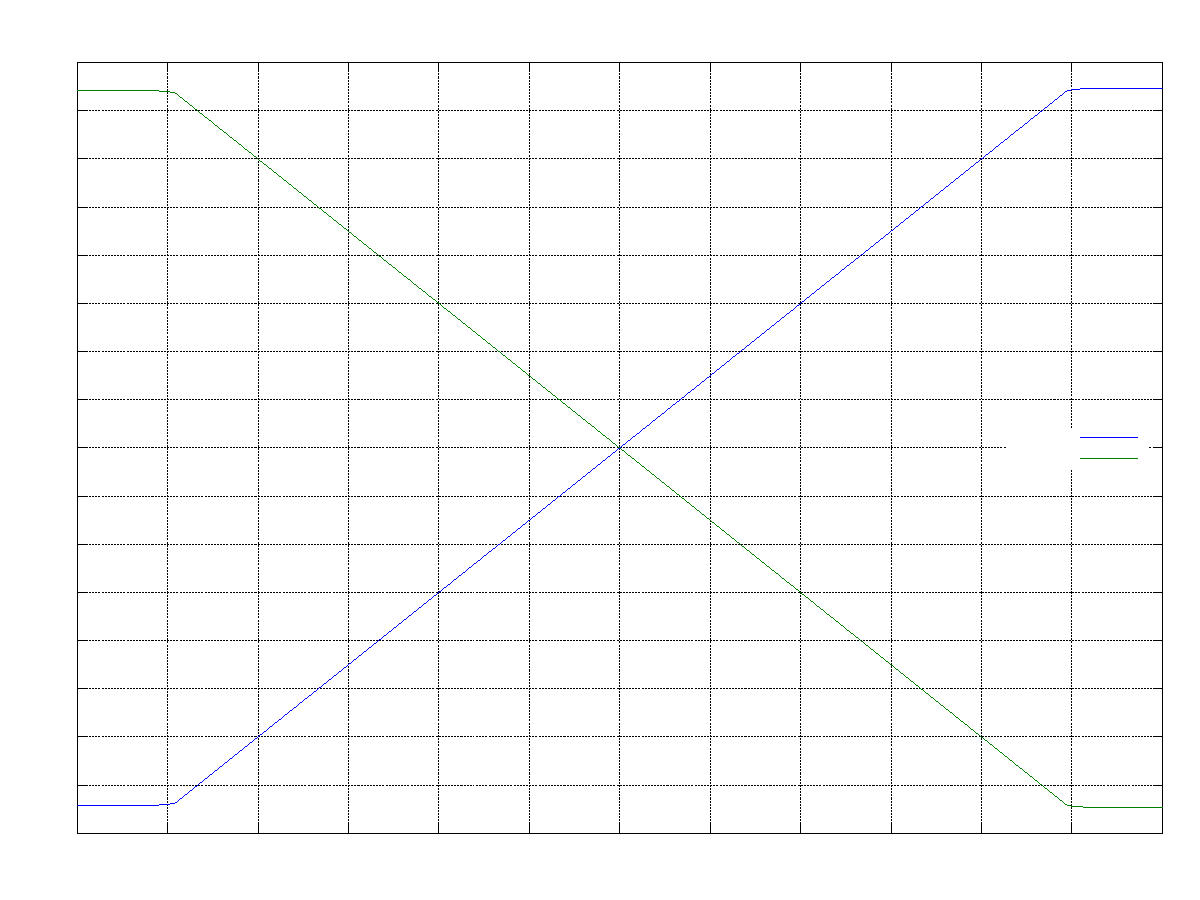
\includegraphics{DCSweep}}%
    \gplfronttext
  \end{picture}%
\endgroup
}
	\caption{DC Transfer Function of the Differential Output Amplifier obtained using LTspice\textsuperscript{\textregistered}\label{fig:DCSweep}}
\end{figure}

A transient simulation of a waveform used in~\cite{Olivo} was also performed.  Figure~\ref{fig:DiffAmpTransSchem} shows the output connected to single-ended loads $Rse1$ and $Rse2$ and differential load $Rd$.  A $0.2\unit{ms}$ wide pulse from midscale DAC output to an amplitude of $1.5\unit{V}$ with a slew rate of $1.5\unit{V}/ \unit{\mu s}$~\cite{AD5678ds} was simulated as a DAC output.  The input waveform and differential and single ended outputs are shown in Figure~\ref{fig:DiffAmpTransSim}.

\begin{figure}[H]
	\begin{singlespace}
	\centering 
		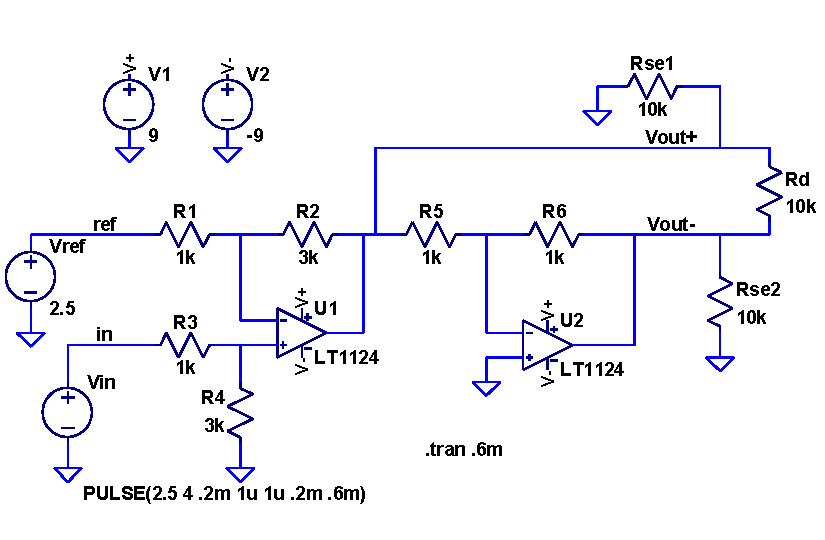
\includegraphics{./figures/LTSchemTrans} 
	\caption{LTspice\textsuperscript{\textregistered} schematic of the Differential Output Amplifier for transient response simulation with single-ended load resistors $Rse1$ and $Rse2$ and differential load resistor $Rd$\label{fig:DiffAmpTransSchem}}
	\end{singlespace}
\end{figure}

\begin{figure}[H]
	\begin{singlespace}
	\centering 
		\resizebox{\textwidth-0.5in}{!}{% GNUPLOT: LaTeX picture with Postscript
\begingroup
  \makeatletter
  \providecommand\color[2][]{%
    \GenericError{(gnuplot) \space\space\space\@spaces}{%
      Package color not loaded in conjunction with
      terminal option `colourtext'%
    }{See the gnuplot documentation for explanation.%
    }{Either use 'blacktext' in gnuplot or load the package
      color.sty in LaTeX.}%
    \renewcommand\color[2][]{}%
  }%
  \providecommand\includegraphics[2][]{%
    \GenericError{(gnuplot) \space\space\space\@spaces}{%
      Package graphicx or graphics not loaded%
    }{See the gnuplot documentation for explanation.%
    }{The gnuplot epslatex terminal needs graphicx.sty or graphics.sty.}%
    \renewcommand\includegraphics[2][]{}%
  }%
  \providecommand\rotatebox[2]{#2}%
  \@ifundefined{ifGPcolor}{%
    \newif\ifGPcolor
    \GPcolorfalse
  }{}%
  \@ifundefined{ifGPblacktext}{%
    \newif\ifGPblacktext
    \GPblacktexttrue
  }{}%
  % define a \g@addto@macro without @ in the name:
  \let\gplgaddtomacro\g@addto@macro
  % define empty templates for all commands taking text:
  \gdef\gplbacktext{}%
  \gdef\gplfronttext{}%
  \makeatother
  \ifGPblacktext
    % no textcolor at all
    \def\colorrgb#1{}%
    \def\colorgray#1{}%
  \else
    % gray or color?
    \ifGPcolor
      \def\colorrgb#1{\color[rgb]{#1}}%
      \def\colorgray#1{\color[gray]{#1}}%
      \expandafter\def\csname LTw\endcsname{\color{white}}%
      \expandafter\def\csname LTb\endcsname{\color{black}}%
      \expandafter\def\csname LTa\endcsname{\color{black}}%
      \expandafter\def\csname LT0\endcsname{\color[rgb]{1,0,0}}%
      \expandafter\def\csname LT1\endcsname{\color[rgb]{0,1,0}}%
      \expandafter\def\csname LT2\endcsname{\color[rgb]{0,0,1}}%
      \expandafter\def\csname LT3\endcsname{\color[rgb]{1,0,1}}%
      \expandafter\def\csname LT4\endcsname{\color[rgb]{0,1,1}}%
      \expandafter\def\csname LT5\endcsname{\color[rgb]{1,1,0}}%
      \expandafter\def\csname LT6\endcsname{\color[rgb]{0,0,0}}%
      \expandafter\def\csname LT7\endcsname{\color[rgb]{1,0.3,0}}%
      \expandafter\def\csname LT8\endcsname{\color[rgb]{0.5,0.5,0.5}}%
    \else
      % gray
      \def\colorrgb#1{\color{black}}%
      \def\colorgray#1{\color[gray]{#1}}%
      \expandafter\def\csname LTw\endcsname{\color{white}}%
      \expandafter\def\csname LTb\endcsname{\color{black}}%
      \expandafter\def\csname LTa\endcsname{\color{black}}%
      \expandafter\def\csname LT0\endcsname{\color{black}}%
      \expandafter\def\csname LT1\endcsname{\color{black}}%
      \expandafter\def\csname LT2\endcsname{\color{black}}%
      \expandafter\def\csname LT3\endcsname{\color{black}}%
      \expandafter\def\csname LT4\endcsname{\color{black}}%
      \expandafter\def\csname LT5\endcsname{\color{black}}%
      \expandafter\def\csname LT6\endcsname{\color{black}}%
      \expandafter\def\csname LT7\endcsname{\color{black}}%
      \expandafter\def\csname LT8\endcsname{\color{black}}%
    \fi
  \fi
  \setlength{\unitlength}{0.0500bp}%
  \begin{picture}(11520.00,8640.00)%
    \gplgaddtomacro\gplbacktext{%
      \colorrgb{0.00,0.00,0.00}%
      \put(1377,5312){\makebox(0,0)[r]{\strut{}0}}%
      \colorrgb{0.00,0.00,0.00}%
      \put(1377,5848){\makebox(0,0)[r]{\strut{}1}}%
      \colorrgb{0.00,0.00,0.00}%
      \put(1377,6384){\makebox(0,0)[r]{\strut{}2}}%
      \colorrgb{0.00,0.00,0.00}%
      \put(1377,6919){\makebox(0,0)[r]{\strut{}3}}%
      \colorrgb{0.00,0.00,0.00}%
      \put(1377,7455){\makebox(0,0)[r]{\strut{}4}}%
      \colorrgb{0.00,0.00,0.00}%
      \put(1377,7991){\makebox(0,0)[r]{\strut{}5}}%
      \colorrgb{0.00,0.00,0.00}%
      \put(1497,4844){\makebox(0,0){\strut{}0}}%
      \colorrgb{0.00,0.00,0.00}%
      \put(2140,4844){\makebox(0,0){\strut{}0.1}}%
      \colorrgb{0.00,0.00,0.00}%
      \put(2782,4844){\makebox(0,0){\strut{}0.2}}%
      \colorrgb{0.00,0.00,0.00}%
      \put(3425,4844){\makebox(0,0){\strut{}0.3}}%
      \colorrgb{0.00,0.00,0.00}%
      \put(4067,4844){\makebox(0,0){\strut{}0.4}}%
      \colorrgb{0.00,0.00,0.00}%
      \put(4710,4844){\makebox(0,0){\strut{}0.5}}%
      \colorrgb{0.00,0.00,0.00}%
      \put(5352,4844){\makebox(0,0){\strut{}0.6}}%
      \colorrgb{0.00,0.00,0.00}%
      \put(1037,6517){\rotatebox{90}{\makebox(0,0){\strut{}Voltage ($V$)}}}%
      \colorrgb{0.00,0.00,0.00}%
      \put(3424,4544){\makebox(0,0){\strut{}Time ($ms$)}}%
      \csname LTb\endcsname%
      \put(3424,8291){\makebox(0,0){\strut{}Input Voltage $Vin$}}%
    }%
    \gplgaddtomacro\gplfronttext{%
    }%
    \gplgaddtomacro\gplbacktext{%
      \colorrgb{0.00,0.00,0.00}%
      \put(6450,5312){\makebox(0,0)[r]{\strut{}0}}%
      \colorrgb{0.00,0.00,0.00}%
      \put(6450,5848){\makebox(0,0)[r]{\strut{}2}}%
      \colorrgb{0.00,0.00,0.00}%
      \put(6450,6384){\makebox(0,0)[r]{\strut{}4}}%
      \colorrgb{0.00,0.00,0.00}%
      \put(6450,6919){\makebox(0,0)[r]{\strut{}6}}%
      \colorrgb{0.00,0.00,0.00}%
      \put(6450,7455){\makebox(0,0)[r]{\strut{}8}}%
      \colorrgb{0.00,0.00,0.00}%
      \put(6450,7991){\makebox(0,0)[r]{\strut{}10}}%
      \colorrgb{0.00,0.00,0.00}%
      \put(6570,4844){\makebox(0,0){\strut{}0}}%
      \colorrgb{0.00,0.00,0.00}%
      \put(7212,4844){\makebox(0,0){\strut{}0.1}}%
      \colorrgb{0.00,0.00,0.00}%
      \put(7855,4844){\makebox(0,0){\strut{}0.2}}%
      \colorrgb{0.00,0.00,0.00}%
      \put(8497,4844){\makebox(0,0){\strut{}0.3}}%
      \colorrgb{0.00,0.00,0.00}%
      \put(9139,4844){\makebox(0,0){\strut{}0.4}}%
      \colorrgb{0.00,0.00,0.00}%
      \put(9782,4844){\makebox(0,0){\strut{}0.5}}%
      \colorrgb{0.00,0.00,0.00}%
      \put(10424,4844){\makebox(0,0){\strut{}0.6}}%
      \colorrgb{0.00,0.00,0.00}%
      \put(5990,6517){\rotatebox{90}{\makebox(0,0){\strut{}Voltage ($V$)}}}%
      \colorrgb{0.00,0.00,0.00}%
      \put(8497,4544){\makebox(0,0){\strut{}Time ($ms$)}}%
      \csname LTb\endcsname%
      \put(8497,8291){\makebox(0,0){\strut{}Differential Output Voltage $Vout+$ to $Vout-$}}%
    }%
    \gplgaddtomacro\gplfronttext{%
    }%
    \gplgaddtomacro\gplbacktext{%
      \colorrgb{0.00,0.00,0.00}%
      \put(1377,1161){\makebox(0,0)[r]{\strut{}-6}}%
      \colorrgb{0.00,0.00,0.00}%
      \put(1377,1582){\makebox(0,0)[r]{\strut{}-4}}%
      \colorrgb{0.00,0.00,0.00}%
      \put(1377,2003){\makebox(0,0)[r]{\strut{}-2}}%
      \colorrgb{0.00,0.00,0.00}%
      \put(1377,2424){\makebox(0,0)[r]{\strut{}0}}%
      \colorrgb{0.00,0.00,0.00}%
      \put(1377,2845){\makebox(0,0)[r]{\strut{}2}}%
      \colorrgb{0.00,0.00,0.00}%
      \put(1377,3266){\makebox(0,0)[r]{\strut{}4}}%
      \colorrgb{0.00,0.00,0.00}%
      \put(1377,3687){\makebox(0,0)[r]{\strut{}6}}%
      \colorrgb{0.00,0.00,0.00}%
      \put(1497,750){\makebox(0,0){\strut{}0}}%
      \colorrgb{0.00,0.00,0.00}%
      \put(2140,750){\makebox(0,0){\strut{}0.1}}%
      \colorrgb{0.00,0.00,0.00}%
      \put(2782,750){\makebox(0,0){\strut{}0.2}}%
      \colorrgb{0.00,0.00,0.00}%
      \put(3425,750){\makebox(0,0){\strut{}0.3}}%
      \colorrgb{0.00,0.00,0.00}%
      \put(4067,750){\makebox(0,0){\strut{}0.4}}%
      \colorrgb{0.00,0.00,0.00}%
      \put(4710,750){\makebox(0,0){\strut{}0.5}}%
      \colorrgb{0.00,0.00,0.00}%
      \put(5352,750){\makebox(0,0){\strut{}0.6}}%
      \colorrgb{0.00,0.00,0.00}%
      \put(917,2423){\rotatebox{90}{\makebox(0,0){\strut{}Voltage ($V$)}}}%
      \colorrgb{0.00,0.00,0.00}%
      \put(3424,450){\makebox(0,0){\strut{}Time ($ms$)}}%
      \csname LTb\endcsname%
      \put(3424,4197){\makebox(0,0){\strut{}Single-ended Output Voltage $Vout+$ to $AGND$}}%
    }%
    \gplgaddtomacro\gplfronttext{%
    }%
    \gplgaddtomacro\gplbacktext{%
      \colorrgb{0.00,0.00,0.00}%
      \put(6450,1161){\makebox(0,0)[r]{\strut{}-6}}%
      \colorrgb{0.00,0.00,0.00}%
      \put(6450,1582){\makebox(0,0)[r]{\strut{}-4}}%
      \colorrgb{0.00,0.00,0.00}%
      \put(6450,2003){\makebox(0,0)[r]{\strut{}-2}}%
      \colorrgb{0.00,0.00,0.00}%
      \put(6450,2424){\makebox(0,0)[r]{\strut{}0}}%
      \colorrgb{0.00,0.00,0.00}%
      \put(6450,2845){\makebox(0,0)[r]{\strut{}2}}%
      \colorrgb{0.00,0.00,0.00}%
      \put(6450,3266){\makebox(0,0)[r]{\strut{}4}}%
      \colorrgb{0.00,0.00,0.00}%
      \put(6450,3687){\makebox(0,0)[r]{\strut{}6}}%
      \colorrgb{0.00,0.00,0.00}%
      \put(6570,750){\makebox(0,0){\strut{}0}}%
      \colorrgb{0.00,0.00,0.00}%
      \put(7212,750){\makebox(0,0){\strut{}0.1}}%
      \colorrgb{0.00,0.00,0.00}%
      \put(7855,750){\makebox(0,0){\strut{}0.2}}%
      \colorrgb{0.00,0.00,0.00}%
      \put(8497,750){\makebox(0,0){\strut{}0.3}}%
      \colorrgb{0.00,0.00,0.00}%
      \put(9139,750){\makebox(0,0){\strut{}0.4}}%
      \colorrgb{0.00,0.00,0.00}%
      \put(9782,750){\makebox(0,0){\strut{}0.5}}%
      \colorrgb{0.00,0.00,0.00}%
      \put(10424,750){\makebox(0,0){\strut{}0.6}}%
      \colorrgb{0.00,0.00,0.00}%
      \put(5990,2423){\rotatebox{90}{\makebox(0,0){\strut{}Voltage ($V$)}}}%
      \colorrgb{0.00,0.00,0.00}%
      \put(8497,450){\makebox(0,0){\strut{}Time ($ms$)}}%
      \csname LTb\endcsname%
      \put(8497,4197){\makebox(0,0){\strut{}Single-ended Output Voltage $Vout-$ to $AGND$}}%
    }%
    \gplgaddtomacro\gplfronttext{%
    }%
    \gplbacktext
    \put(0,0){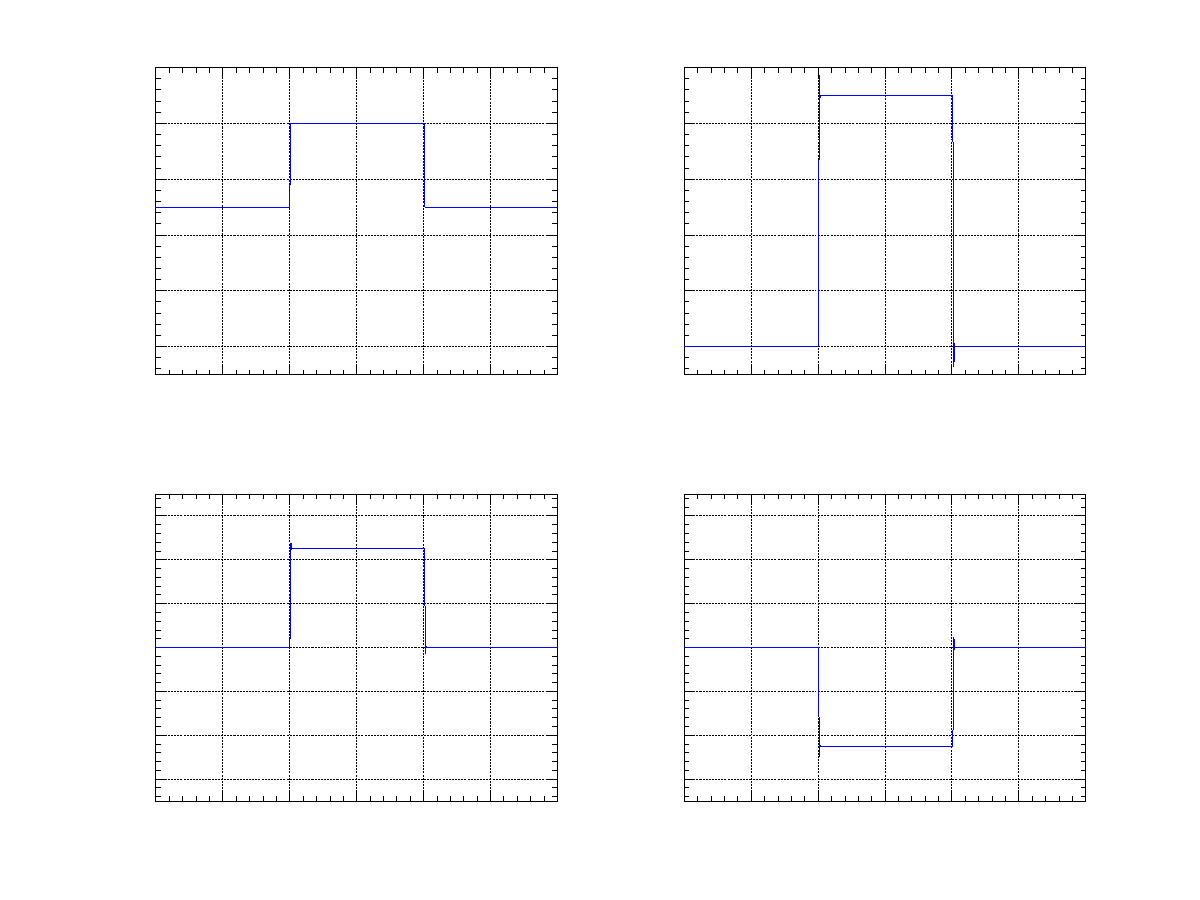
\includegraphics{DiffOutAmpTrans}}%
    \gplfronttext
  \end{picture}%
\endgroup
}
	\caption{Differential Output Amplifier transient response to a $0.2\unit{ms}$ pulse from a DAC output obtained using LTspice\textsuperscript{\textregistered}\label{fig:DiffAmpTransSim}}
	\end{singlespace}
\end{figure}


\subsubsection{Analog to Digital Converter}\label{sec:adc}

%Description of ADC connections to the FPGA
The analog to digital converter (ADC) is responsible for converting the analog voltage from the output of the Preamp, which is connected to the recording electrodes in the electrophysiology setup, into digital values at regular discrete time intervals.  According to the sampling theorem, the sampling frequency must be at least twice the highest frequency component of the analog signal to avoid loss of information in the analog to digital conversion~\cite{AlexanderSadiku2004}.  The Preamp has an output bandwidth of 20\unit{Hz} to 14.6\unit{kHz}~\cite{StahlMSEE}, which means that the minimum required sampling frequency, or Nyquist frequency, of the ADC must be $2\times14.6\unit{kHz}=29.2\unit{kHz}$~\cite{AlexanderSadiku2004}.  The AD7606 ADC from Analog Devices\textsuperscript{\textregistered} offers eight analog inputs with a selectable range of $\pm 10\unit{V}$ or $\pm 5\unit{V}$ with 16 bits of resolution that sample at up to $200\unit{kHz}$~\cite{AD7606ds}, and the AD7606 has been used previously in the Neurobiology Engineering Laboratory~\cite{BatzerCorsiCrampton}.  The AD7606 has an analog input filter with a corner frequency of $23\unit{kHz}$ at $\pm 10\unit{V}$ input range and $15\unit{kHz}$ at $\pm 5\unit{V}$ input range~\cite{BatzerCorsiCrampton}.

Figure~\ref{fig:ADC} shows the connections between the Xilinx\textsuperscript{\textregistered} XC3S500E FPGA on the RTSC board and the AD7606 on the Electrophysiology Interface board.  The FPGA GPIO pins connect to the digital interface of the AD7606 through the Hirose FX2 connectors and the signals are accessible on the 40-pin test header before going through a $0\unit{\Omega}$ resistor and finally connecting to the AD7606.  Signals not used in the FPGA configuration may have their $0\unit{\Omega}$ resistors unpopulated allowing the unused FPGA GPIO pins to be used for other purposes and accessed on the 40-pin test header.  There is a separate power supply pin, VDrive, on the AD7606 that drives the logic outputs and controls the thresholds of the logic inputs; VDrive should be powered to the same voltage as the GPIO supply of the FPGA~\cite{AD7606ds}.

\begin{figure}[H]
	\centering 
		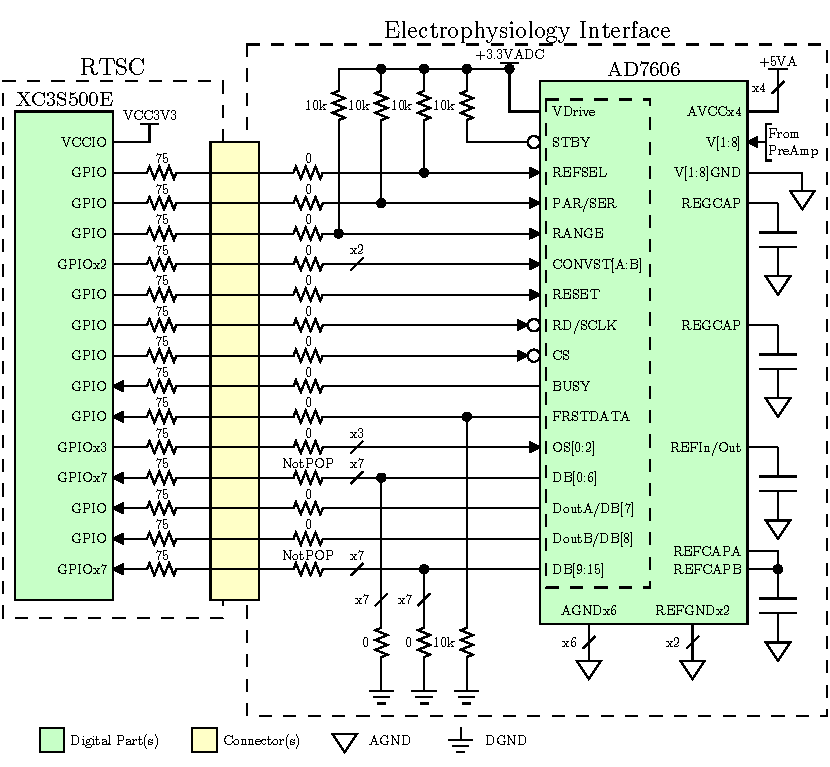
\includegraphics{./figures/AD} 
	\caption{FPGA connections to the ADC\label{fig:ADC}}
\end{figure}

The single-ended outputs of the Preamps are connected to the analog voltage inputs with all channel GND pins connected to AGND.  The main power supply is required to be $5\unit{V}$ $\pm 0.25\unit{V}$~\cite{AD7606ds}, so a $5\unit{V}$ regulator driven by +VA provides the AVCC power.  The Electrophysiology Interface board is setup for the AD7606 to use its internal voltage reference.  The AD7606 requires a $10\unit{\mu F}$ capacitor on the REFIn/Out pin for the operation of its internal voltage reference~\cite{AD7606ds}.  There are also a few capacitors needed for internal regulators and references; these pins have capacitors sized and placed according to the recommendation in the data sheet~\cite{AD7606ds}.  The details of the rest of the pin functions and connections are in Table~\ref{tab:AD7606Pins}.

\renewcommand{\arraystretch}{1.3}
%\begin{table}[H]
\begin{singlespace}
\centering 
\begin{longtable}[h]{|p{1.5in}|p{3.5in}|}
\multicolumn{2}{c}{{Table~\ref{tab:AD7606Pins}}} \\
\hline
Pin	& Function\\
\endhead
\multicolumn{2}{r}{\textit{Continued on next page}} \\
\endfoot
\endlastfoot
\hline
VDrive	& Digital supply voltage.  Should be the same voltage as FPGA GPIO\\
\hline
$\overline{\mathrm{STBY}}$	& Puts AD7606 into low power standby mode when LOW.  Tied to HIGH and not connected to FPGA\\
\hline
REFSEL	& Selects internal, HIGH, or external, LOW, voltage reference.  Pulled high through $10\unit{k\Omega}$ so $0\unit{\Omega}$ resistor may be unpopulated and FPGA GPIO used for other purpose\\
\hline
$\overline{\mathrm{PAR}}$/SER/BYTESEL	& Selects between serial, HIGH, or parallel, LOW, data interface.  If parallel interface is selected, this is read in conjunction with DB[15] to specify 8 or 16 bit parallel interface.  Pulled high through $10\unit{k\Omega}$ so $0\unit{\Omega}$ resistor may be unpopulated and FPGA GPIO used for other purpose\\
\hline
RANGE	& Sets analog input range at $\pm10\unit{V}$, HIGH, or $\pm10\unit{V}$, LOW.  Pulled high through $10\unit{k\Omega}$ so $0\unit{\Omega}$ resistor may be unpopulated and FPGA GPIO used for other purpose\\
\hline
CONVST[A:B]	& Conversion Start A initiates conversions on the lower half of the analog inputs (channels 1-4 for AD7606, 1-3 for AD7606-6, and 1-2 for AD7606-4) and Conversion Start B initiates conversions on the upper half of the analog inputs.  To sample on all channels simultaneously, switch both signals simultaneously.  These can be shorted if both are always going to be started simultaneously, saving a FPGA GPIO pin.\\
\hline
RESET	& Rising edge resets the AD7606.  The FPGA should issue a RESET pulse to the AD7606 upon power-up\\
\hline
$\overline{\mathrm{RD}}$/SCLK	& Parallel data read control or serial data clock input\\
\hline
$\overline{\mathrm{CS}}$	& Chip select input frames data transfer\\
\hline
BUSY	& Output rises after CONVST and falls after conversion is complete and data is ready to be clocked out\\
\hline
FRSTDATA	& Three-state output is high-impedance when $\overline{\mathrm{CS}}$ is HIGH, when $\overline{\mathrm{CS}}$ is LOW, FRSTDATA is LOW except during the $\overline{\mathrm{RD}}$ operation when channel 1 is on the parallel interface or when the 16 bits of channel 1 are being clocked out of DoutA on the serial interface (see~\cite{AD7606ds} for more information).  Pulled low through $10\unit{k\Omega}$ resistor to keep signal at known state when in three(tri)-state (high-impedance) mode.\\
\hline
OS[0:2]	& Over sampling mode select pins enables conversion a high sampling frequency and reading of the data at a lower frequency.  The AD7606 then applies a digital low-pass filter before making the data available on the parallel or serial interface.  Setting the mode pins to [0:0:0] disables the over sampling function.  Enabling the over sampling function affects effective input bandwidth.\\
\hline
DB[0:6]	& Three-state parallel digital input/output pins that should be tied to ground if serial data interface is used.  If using the AD7606 in serial mode $0\unit{\Omega}$ resistors to ground should be populated and $0\unit{\Omega}$ resistors to the FPGA should not be populated.  If using the AD7606 in parallel mode $0\unit{\Omega}$ resistors to ground should not be populated and $0\unit{\Omega}$ resistors to the FPGA should be populated.\\
\hline
DoutA/DB[7]	& If $\overline{\mathrm{PAR}}$/SER/BYTESEL is HIGH, it functions as DoutA and outputs serial conversion data. Channels 1 to 4 (1 to 3 for AD7606-6, 1 to 2 for AD7606-4) first appear on DoutA.  If $\overline{\mathrm{PAR}}$/SER/BYTESEL is LOW it's a three-state parallel digital input/output pin.\\
\hline
DoutB/DB[8]	& If $\overline{\mathrm{PAR}}$/SER/BYTESEL is HIGH, it functions as DoutB and outputs serial conversion data. Channels 1 to 4 (5 to 8 for AD7606-6, 3 to 4 for AD7606-4) first appear on DoutB. Can be used as a single Dout line, the channels appear in order 5-8 then 1-4.  If $\overline{\mathrm{PAR}}$/SER/BYTESEL is LOW it's a three-state parallel digital input/output pin.\\
\hline
DB[9:15]	& DB[15] is also an input pin and is read if $\overline{\mathrm{PAR}}$/SER/BYTESEL is LOW to select between 8 bit and 16 bit interface.  Three-state parallel digital input/output pins that should be tied to ground if serial data interface is used.  If using the AD7606 in serial mode $0\unit{\Omega}$ resistors to ground should be populated and $0\unit{\Omega}$ resistors to the FPGA should not be populated.  If using the AD7606 in parallel mode $0\unit{\Omega}$ resistors to ground should not be populated and $0\unit{\Omega}$ resistors to the FPGA should be populated.\\
\hline
REGCAP	& Decoupling capacitors for internal regulators.  Each pin should have a $1\unit{\mu F}$ capacitor as close to the pin as possible with the other end connected to ground.\\
\hline
REFIn/Out	& Voltage reference in or out.  The pin should have a $10\unit{\mu F}$ capacitor as close to the pin as possible with the other end connected to ground.\\
\hline
REFCAP[A:B]	& Reference buffer output force/sense pins.  These pins should be tied together and have a $10\unit{\mu F}$ low ESR, ceramic capacitor as close to the pin as possible with the other end connected to ground.\\
\hline

\caption{Notes on AD7606 ADC pin connections and functions with information from~\cite{AD7606ds}\label{tab:AD7606Pins} }
\end{longtable}


\end{singlespace}
%\end{table}
\renewcommand{\arraystretch}{1.0}



\subsubsection{Preamp Interface}\label{sec:preamp}

%Description of PCI-Express connections to the Preamp and the relevant signals to/from the differential output amplifier, ADC, and CPLD
Action potentials in electrophysiological systems are very low amplitude in the order of $10\unit{\mu V}$ to $100\unit{\mu V}$~\cite{Potter2005}.  To study the electrophysiological signals with electrical equipment, the first step is to amplify the low voltage action potentials.  Previous work on this has been done in the Neurobiology Engineering Laboratory yielding a low noise amplifier design~\cite{StahlMSEE,BatzerCorsiCrampton}.  Since then, the design has been adapted to fit on a PCB with a card edge connector compatible with 36-pin connectors designed for PCI-Express cards but with a custom pinout.  This approach allows the tested Preamp design to be built independently of the rest of the experimental system, and eliminates the need to replicate the sensitive circuit that can be susceptible to noise.  Pictures of the card edge connector version of the Preamp board, provided by John Stahl, are shown in Figure~\ref{fig:PreampBoard}.

\begin{figure}[h]
	\centering 
	\begin{singlespace}
	\begin{subfigure}[b]{\textwidth}
		\centering 
		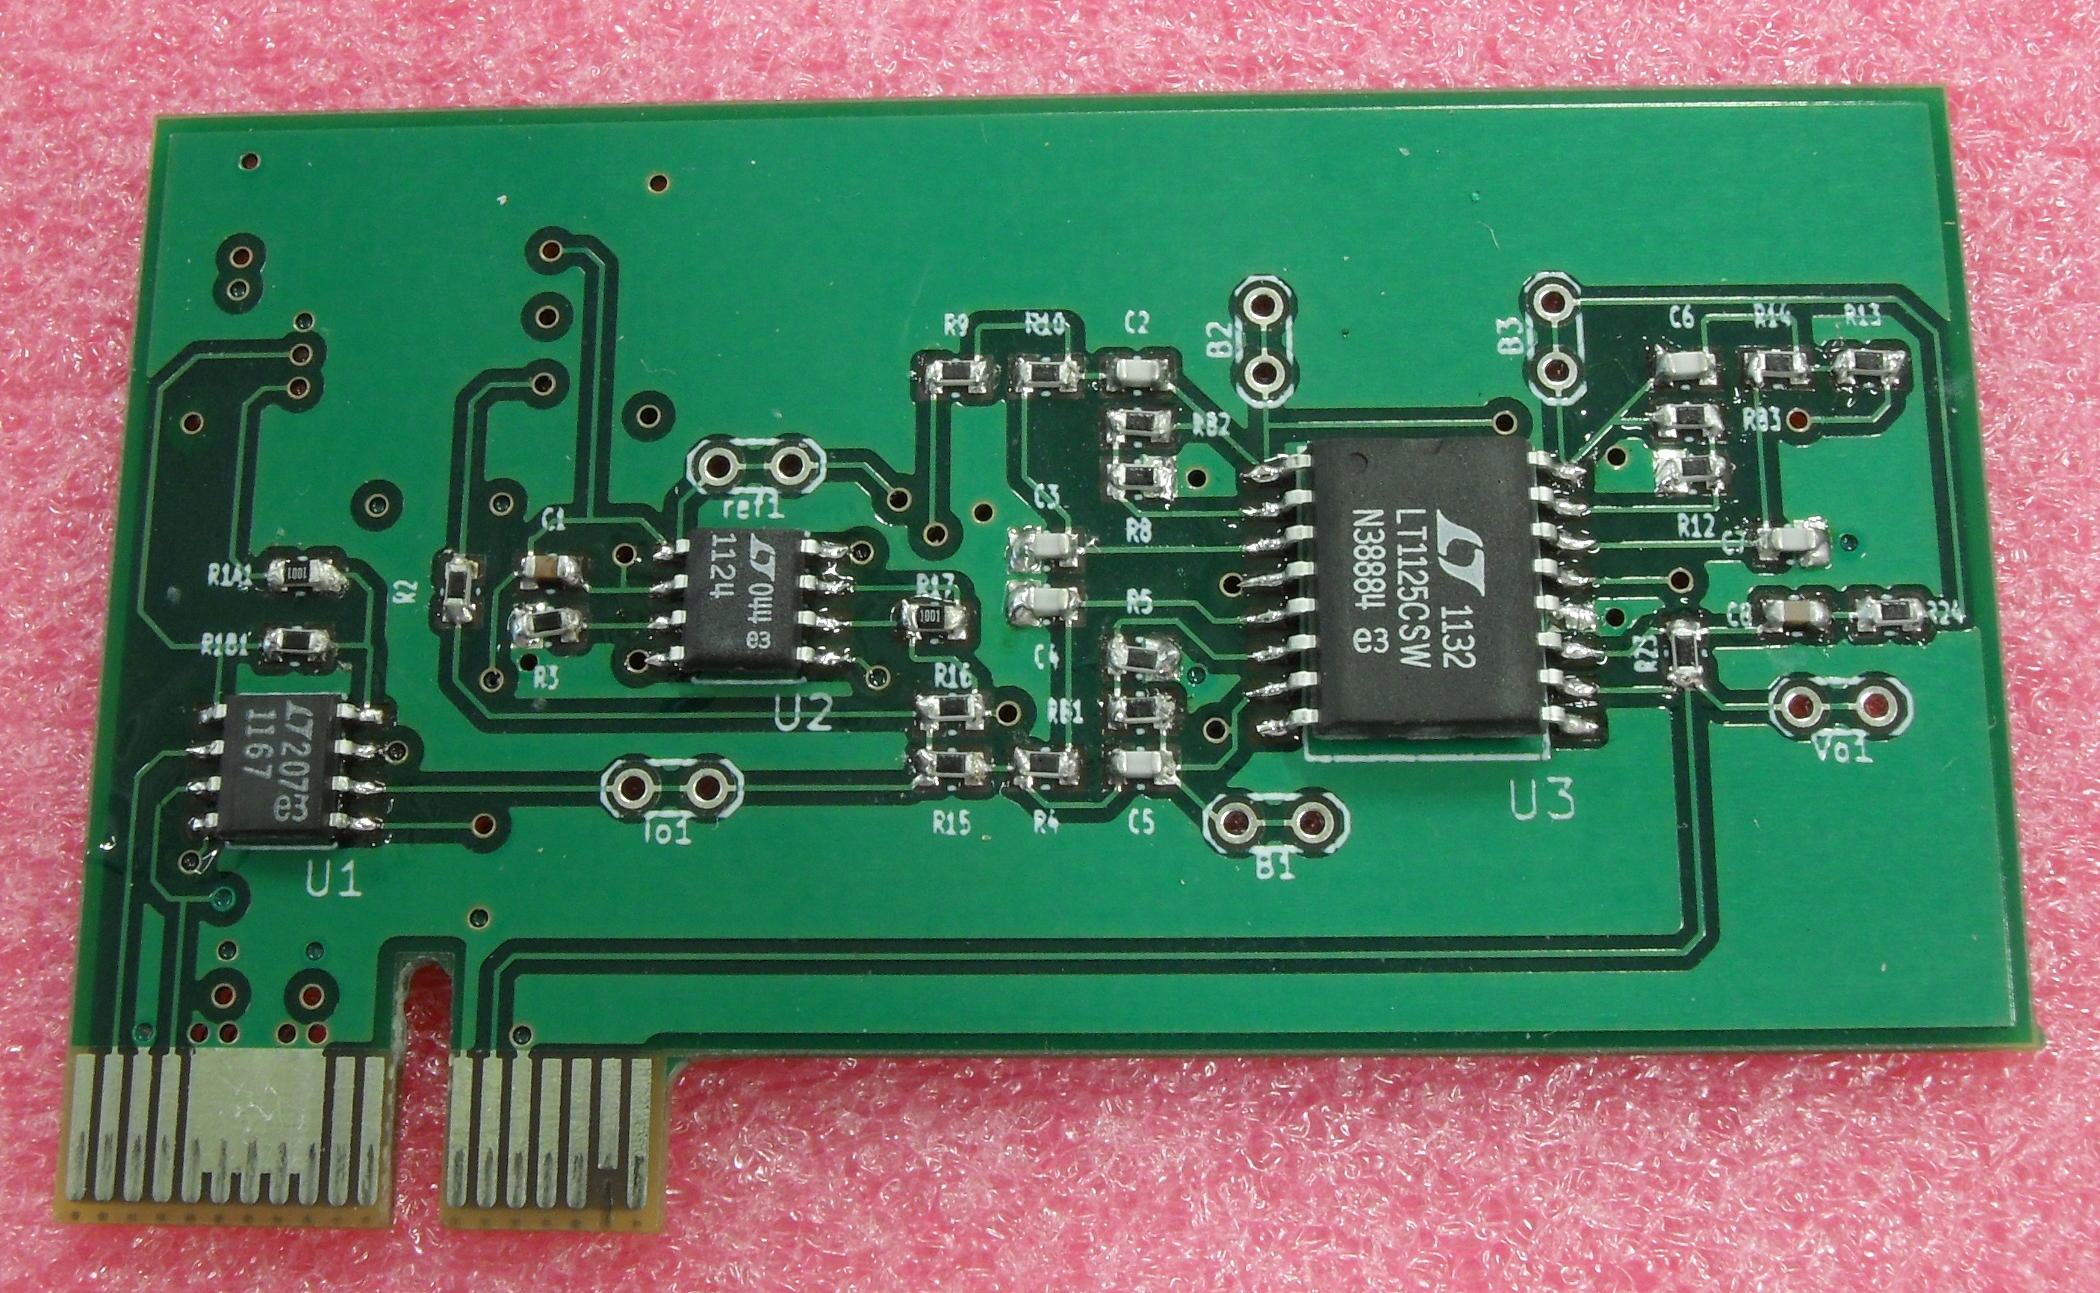
\includegraphics{./figures/PreAmpTop} 
	\caption{Top side\label{fig:patop}}
	\end{subfigure}
	\\
	\begin{subfigure}[b]{\textwidth}
		\centering 
		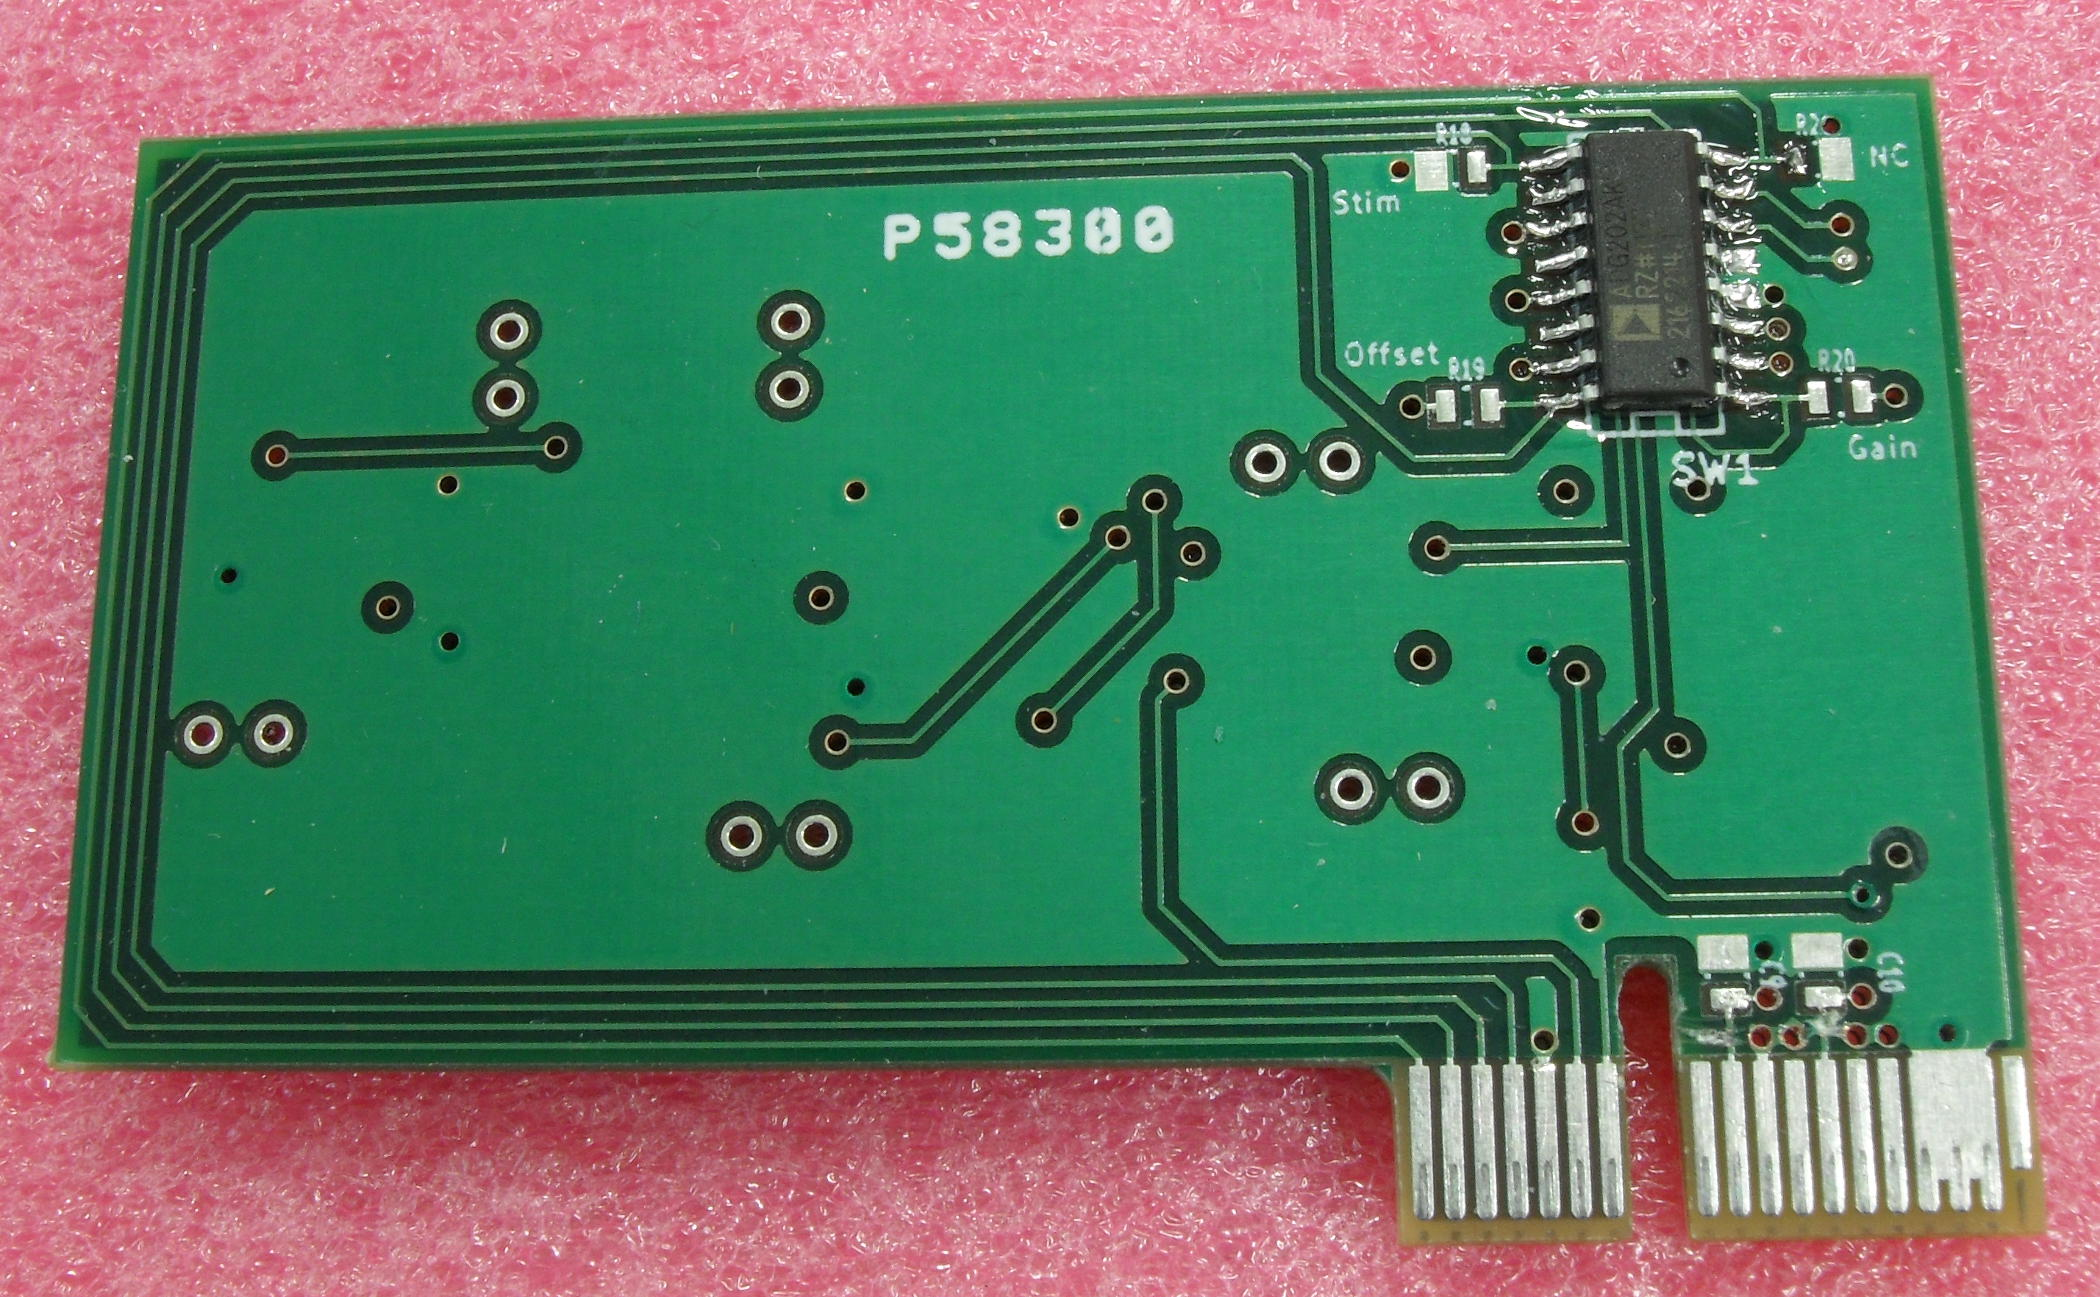
\includegraphics{./figures/PreAmpBot} 
	\caption{Bottom Side\label{fig:pabot}}
	\end{subfigure}
	\caption{Views of a populated Preamp Board with card edge connector, provided by John Stahl\label{fig:PreampBoard}}
	\end{singlespace}
\end{figure}

A block diagram of the Preamp board, based on~\cite{Jimbo2003,StahlMSEE}, is shown in Figure~\ref{fig:PreampInt} along with its connection to the Electrophysiology Interface board.  Not shown is the analog power and ground connections to the Preamp.  A summary of the connections is shown in Table~\ref{tab:PreampInt}.

\begin{figure}[h!]
	\centering 
		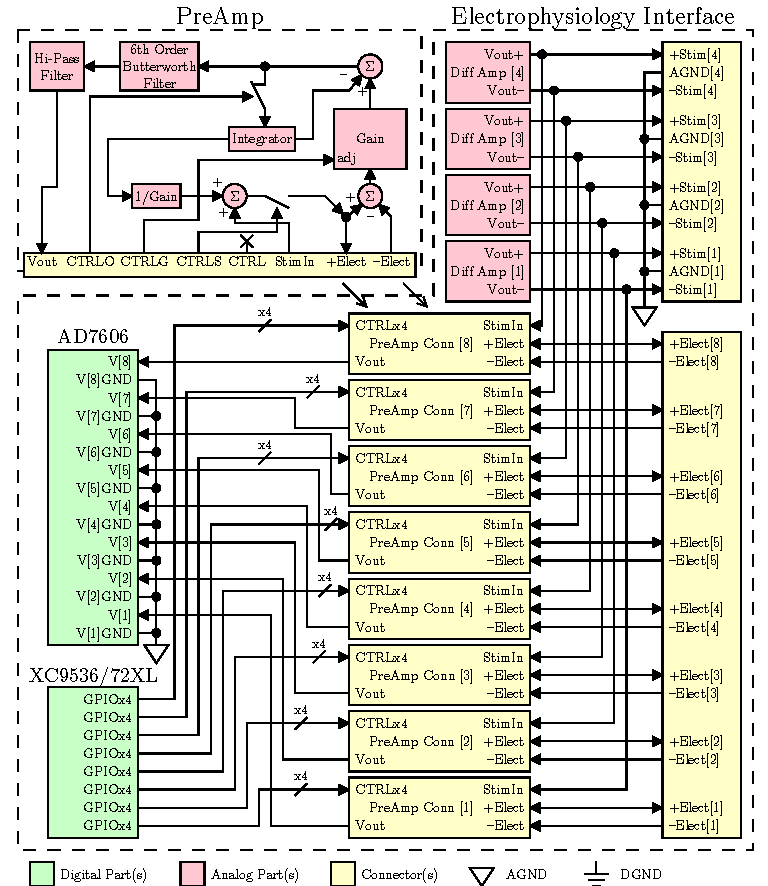
\includegraphics{./figures/PreAmpInt} 
	\caption{Preamp block diagram~\cite{Jimbo2003, StahlMSEE} and Electrophysiology Interface board connections\label{fig:PreampInt}}
\end{figure}

\renewcommand{\arraystretch}{1.3}
\begin{table}[h]
\centering 
\begin{tabular}{|l|l|p{3.5in}|}
\hline
Signal	&	Connector Pin	& Function\\
\hline
+Elect	& B4	& Non-inverting input of low-noise instrumentation amplifier\\
\hline
$-\mathrm{Elect}$	& B2	& Inverting input of low-noise instrumentation amplifier\\
\hline
StimIn	& A13	& Single-ended stimulation input that can be routed to the non-inverting input\\
\hline
Vout	& B13	& Single-ended output of the Preamp\\
\hline
CTRLO	& A15	& Digital input controls AC coupling integrator\\
\hline
CTRLS	& A16	& Digital input controls connecting summing amplifier to non-inverting input\\
\hline
CTRLG	& A17	& Digital input controls gain of instrumentation amplifier\\
\hline
CTRL	& A18	& Digital input controls unused analog switch.  Included for any future design needs\\
\hline
V+	& B10	& Positive analog voltage supply for Preamp circuits.  Connected to +VA supply on Electrophysiology Interface board\\
\hline
$\mathrm{V}-$	& B8	& Negative analog voltage supply for Preamp circuits.  Connected to $-\mathrm{VA}$ supply on Electrophysiology Interface board\\
\hline
GND	& All others	& Remaining pins on connector are used to connect to circuit ground.  Connected to AGND on Electrophysiology Interface board \\
\hline
\end{tabular}
\caption{Preamp PCI-Express 36-pin connector signals and pinout\label{tab:PreampInt} }

\end{table}
\renewcommand{\arraystretch}{1.0}

The Preamp consists of a differential input that is connected to the recording electrodes of the biological system.  The low voltage signal from the electrodes is amplified by a low-noise instrumentation amplifier.  An integrator connected to the instrumentation amplifier subtracts the DC part of the signal which is then passed to a 6th Order Butterworth Filter for additional gain and bandwidth reduction.  A high-pass filter removes any DC component added by the Butterworth Filter circuit, and the result is a single ended output signal.

The Preamp also has the capability of outputting a stimulation signal on the non-inverting electrode with the DC offset of the electrode added to the stimulation signal~\cite{Jimbo2003,StahlMSEE}.  Four digital control signals, with one not used by the Preamp, connected to analog switches and a stimulation input are needed to realize this function.  CTRLO disconnects the integrator from the instrumentation amplifier output so the stimulation signal does not affect the DC offset calculation; CTRLG reduces the gain of the instrumentation amplifier to keep the amplifier from saturating when the comparatively high voltage stimulation signal is added to the electrode; an op-amp circuit adds the DC offset value, which is the integrator output divided by the instrumentation amplifier gain, to the single-ended stimulation signal, StimIn; and, finally, CTRLS connects the summing op-amp to the non-inverting electrode.  The stimulation signal overpowers any biological signals on the recording electrode and allows an artificial signal to be applied to a biological system.  

A summary of the digital signals that control the Preamp stimulation mode is in Table~\ref{tab:PreampStim}.  Pull-up and pull-down resistors are included on the Preamp board to default its behavior to measurement mode.  Tri-stated outputs may be connected to the Preamp's digital inputs for measurement mode.  Additional work may be needed to determine the optimal relative timing of the signals for switching modes~\cite{StahlMSEE}.

\renewcommand{\arraystretch}{1.3}
\begin{table}[hb]
\centering 
\begin{tabular}{|l|l|l|}
\hline
Signal	&	Measurement	& Stimulation\\
\hline
CTRLO	& HIGH or tri-state	& LOW\\
\hline
CTRLS	& LOW or tri-state	& HIGH\\
\hline
CTRLG	& LOW or tri-state	& HIGH\\
\hline
CTRL	& X	& X\\
\hline
\end{tabular}
\caption{Preamp digital control for stimulation mode\label{tab:PreampStim} }

\end{table}
\renewcommand{\arraystretch}{1.0}

A summary of how the Electrophysiology Board is connected to the Preamp, as shown in Figure~\ref{fig:PreampInt}, is now provided. A terminal block connects the biological system measurement electrodes to the Preamp electrode inputs.  Differential or single-ended stimulation signals from the four Differential Output Amplifiers may be connected to the biological system using a terminal block, or the single-ended stimulation signals may be routed to the non-inverting recording electrodes by changing the desired Preamp to stimulation mode.  The output of the Preamps are connected to the analog inputs of the AD7606 ADC.  Not shown in the figure are $0\unit{\Omega}$ resistors that may be used to bypass the Preamp by connecting the non-inverting electrode signal from the terminal block to the input of the ADC (this should only be done when a Preamp board is not in the PCI-Express connector).  A $0\unit{\Omega}$ resistor can also be used to connect the inverting input of the Preamps to AGND.  A Xilinx\textsuperscript{\textregistered} XC9572XL CPLD (or the pin-compatible XC9536XL) connects to all of the control inputs of the Preamps.


\subsubsection{CPLD}\label{sec:cpld}

%Description of the CPLD and its connections to the FPGA and Preamps
Preamp boards have four digital inputs to set their mode for measurement or stimulation.  More experimentation is needed determine optimal relative timing of these inputs~\cite{StahlMSEE}.  The RTSC must have the ability to uniquely control each Preamp digital input, which means, for eight Preamp boards, a total of 32 external IO pins would be required of the Xilinx\textsuperscript{\textregistered} XC3S500E FPGA.  The Hirose FX2 connector on the RTSC exposes 40 IO pins, but many of those are needed for the DAC and ADC interfaces.  Thus, a CPLD provided on the Electrophysiology Interface board, as shown in Figure~\ref{fig:CPLD}, can act as an IO expander allowing the FPGA individual control of the four digital inputs on each of the eight Preamps connected to the Electrophysiology Interface board.

\begin{figure}[H]
	\centering 
		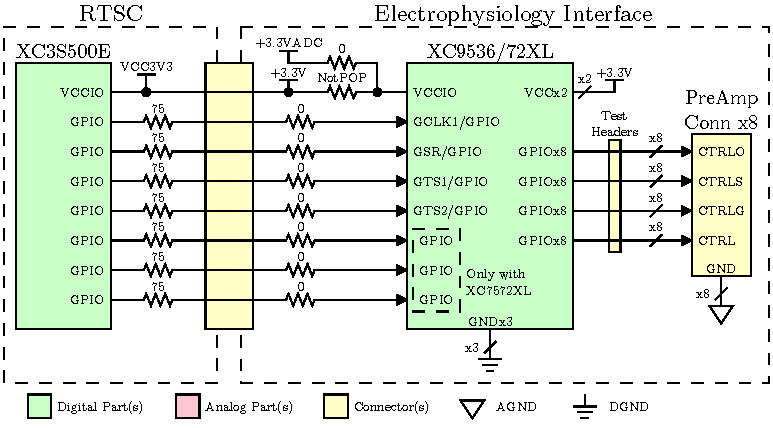
\includegraphics{./figures/CPLD} 
	\caption{Connections between the FPGA on the RTSC board and the CPLD and Preamp Connectors on the Electrophysiology Interface board\label{fig:CPLD}}
\end{figure}

A CPLD solves the problem of scarce IO very well.  The configuration of the CPLD can be changed based on the needs of the system as determined by experimentation: it could be configured to simply change all of the IO pins based on a single input, or it could be configured to respond to a complex serial interface with multiple commands and a clock input.  The XC9500XL series are Xilinx\textsuperscript{\textregistered} CPLD devices that have adequate number of IO pins available, that can be powered with a single $3.3\unit{V}$ voltage supply available on the Electrophysiology Interface board from the RTSC board, that retain their configuration between power cycles, and that use the same tools from Xilinx\textsuperscript{\textregistered} and Digilent\textsuperscript{\textregistered} for configuration, development, and programming as the FGPA on the RTSC board~\cite{XC9500XLds}.

The CPLD used must have enough external IO pins to connect to the eight Preamp boards plus a few IO pins for the interface with the FPGA.  The DAC and ADC use 33 of the 40 available FPGA IO connections leaving seven IO connections for the FPGA to CPLD interface.  Several package options are available for XC9500XL family, but the Quad Flat Pack (xQFP) variations offer the most flexibility in available parts and are relatively easy to solder by hand.  The 44-pin VQFP package offers only 34 external IO pins, which, after connecting the Preamp signals, leaves only 2 pins for the FPGA interface, but the 64-pin VQFP package offers 36 IO pins with the XC9536XL and 52 IO pins with the XC9572XL~\cite{DesignXC9500XLappnote}.  Designing the Electrophysiology Interface board for the XC9572XL in the 64-pin VQFP package will allow the XC9536XL to be used in its place for a cheaper price and lower power consumption, if the extra IO and logic gates offered by the XC9572XL are not needed.  A summary of the capabilities of the XC9536XL versus the XC9572XL on the Electrophysiology Interface board are shown in Table~\ref{tab:CPLDMigration}, which has information from~\cite{XC9500XLds} and~\cite{DesignXC9500XLappnote}.

\renewcommand{\arraystretch}{1.3}
\begin{table}[h]
\centering 
\begin{tabular}{|l|l|l|l|l|l|}

\hline
CPLD	& IO Pins & Macrocells & Gates & Preamp Signals & FPGA Signals\\
\hline
XC9536XL	& 36 & 36 & 800 & 32 & 4\\
\hline
XC9572XL	& 52 & 72 & 1600 & 32 & 7\\
\hline
\end{tabular}
\caption{XC9536XL and XC9572XL VQFP-64 capabilities on the Electrophysiology Interface board~\cite{XC9500XLds,DesignXC9500XLappnote}\label{tab:CPLDMigration} }

\end{table}
\renewcommand{\arraystretch}{1.0}

Four of the signals from the FPGA are connected to special function pins of the CPLD.  These pins provide low-latency operation for the special functions, but may be configured as general purpose IO (GPIO), if the special functions aren't needed.

Test headers provide access to the signals between the CPLD and the Preamp connectors.  There are two internal power supply pins, VCC, that are connected to the $+3.3\unit{V}$ power rail that is connected to the VCC3V3 power supply on the RTSC board.  There is a separate power supply input pin for the IO buffers, VCCIO, that can be connected to $+3.3\unit{V}$ or to the output of the $3.3\unit{V}$ regulator on the Electrophysiology Interface board, labeled as $+3.3\unit{VADC}$.  VCCIO and VCC can be powered in any sequence without harming the part~\cite{DesignXC9500XLappnote}.

The digital inputs on the Preamp boards are connected to an Analog Devices ADG202A quad analog switch IC.  Its digital input requirements are compared to the digital output specifications of the XC9536XL and XC9572XL, with $\mathrm{VCCIO}=3.3\unit{V}$, in Table~\ref{tab:PreampCPLDVolt}, which shows that the CPLD outputs are compatible with the ADG202A inputs~\cite{ADG202Ads,XC9536XLds,XC9572XLds}.

\renewcommand{\arraystretch}{1.3}
\begin{table}[h]
\centering 
\begin{tabular}{|l|l|l|}
\hline
Logic	& HIGH & LOW\\
\hline
ADG202A	Input & $2.4\unit{Vmin}$ & $0.8\unit{Vmax}$\\
\hline
XC9536/72XL	Output & $2.4\unit{Vmin}$ & $0.4\unit{Vmax}$\\
\hline
\end{tabular}
\caption{AD202A quad analog switch and XC9536/72XL CPLD digital input and output compatibility\label{tab:PreampCPLDVolt} }

\end{table}
\renewcommand{\arraystretch}{1.0}

One possible situation that might cause damage to the CPLD when connected to the Preamp Board is the connection of the digital inputs on the Preamp Board to the analog voltage supplies.  The XC9536XL and XC9572XL have a maximum rating on its input and three-state output pins of $5.5\unit{V}$~\cite{XC9536XLds,XC9572XLds}.  If the Preamp board ties a digital input to its positive analog voltage supply, the voltage on the CPLD pins could exceed their maximum rating.  Tieing the digital inputs on the Preamp boards to a HIGH logic level should be accomplished with a voltage divider to ensure that the maximum voltage does not exceed $5.5\unit{V}$.



\section{Building the Electrophysiology Interface Board}\label{sec:build}

%Description of the steps taken to implement the design on a PCB from schematic capture to layout to ordering to testing
To create a durable, reliable, and professional-looking implementation of the Data-Acquisition and Stimulation System hardware, it is desirable to have the Electrophysiology Interface board design implemented on a printed circuit board (PCB).  To create a PCB, a layout of the circuit design is developed and converted to an industry standard file format that can be submitted to a PCB manufacturer who constructs the PCB.  The complexity of the Electrophysiology Interface board circuit design necessitated a four-layer PCB construction, with internal power and ground plane layers that reduce noise emissions and susceptibility while simplifying signal routing and component placement on the top and bottom layers.

Developing the layout of the PCB requires an electronic design automation (EDA) software suite that is capable of working with a complex design implemented on a four-layer PCB and exporting the PCB design to the industry standard Gerber file format.  KiCad is an open-source EDA suite that has been in development since 2006; provides schematic capture, PCB layout design, and Gerber file export at no cost; and is available for all popular operating systems.  Other EDA suites were evaluated: freeware software suites are often tied to a specific manufacturer with no included Gerber file export capabilities, full-featured software often has prohibitively expensive licensing fees or evaluation versions suitable for only small designs, and the other popular open-source suite, gEDA, does not have an official Windows binary distribution. 

Advanced Circuits is the company that manufactured the Electrophysiology Interface PCB based on Gerber files created using KiCad.  The manufacturer was chosen based on its location in the USA, Gerber file acceptance, and attractive student pricing that produces a four-layer board with silkscreen and solder mask for \$66 with no minimum board quantity requirement.



\subsection{Hierarchical Schematic Capture}

%Description of creating the hierarchical schematic 

The first step in designing a PCB is capturing the entire circuit schematic.  A circuit schematic was developed based on the designs for the Electrophysiology Interface board in section~\ref{sec:hardware} and can be seen in appendix~\ref{sec:schematic} on page~\pageref{sec:schematic}.  The schematic capture program of the KiCad EDA suite, Eeschema, handles complex, multi-sheet schematics with a hierarchical structure.

The root sheet of the schematic on page~\pageref{SchematicRev1r0.1} contains most of the input and output connectors, such as the Hirose FX2 connector, which marries the Electrophysiology Interface board to the RTSC board, and the terminal blocks for connecting to the biological electrodes, allowing the overall signal flow to be summarized on one sheet.  To add more sheets to the design, a block is added to the root sheet representing the sheet added to the design hierarchy and referencing a schematic file that defines the contents of the sheet.  Figure~\ref{fig:hblock} shows a hierarchical block on the root sheet that adds the sheet, PreAmpInterface, found on page~\pageref{SchematicRev1r0.2}, to the design hierarchy with its contents pulled from the file, PreAmpInterface.sch, in the project directory.

\begin{figure}[h]
	\begin{singlespace}
	\centering
%	\setlength\fboxsep{0pt}
%	\setlength\fboxrule{0.5pt}
%	\fbox{ }
	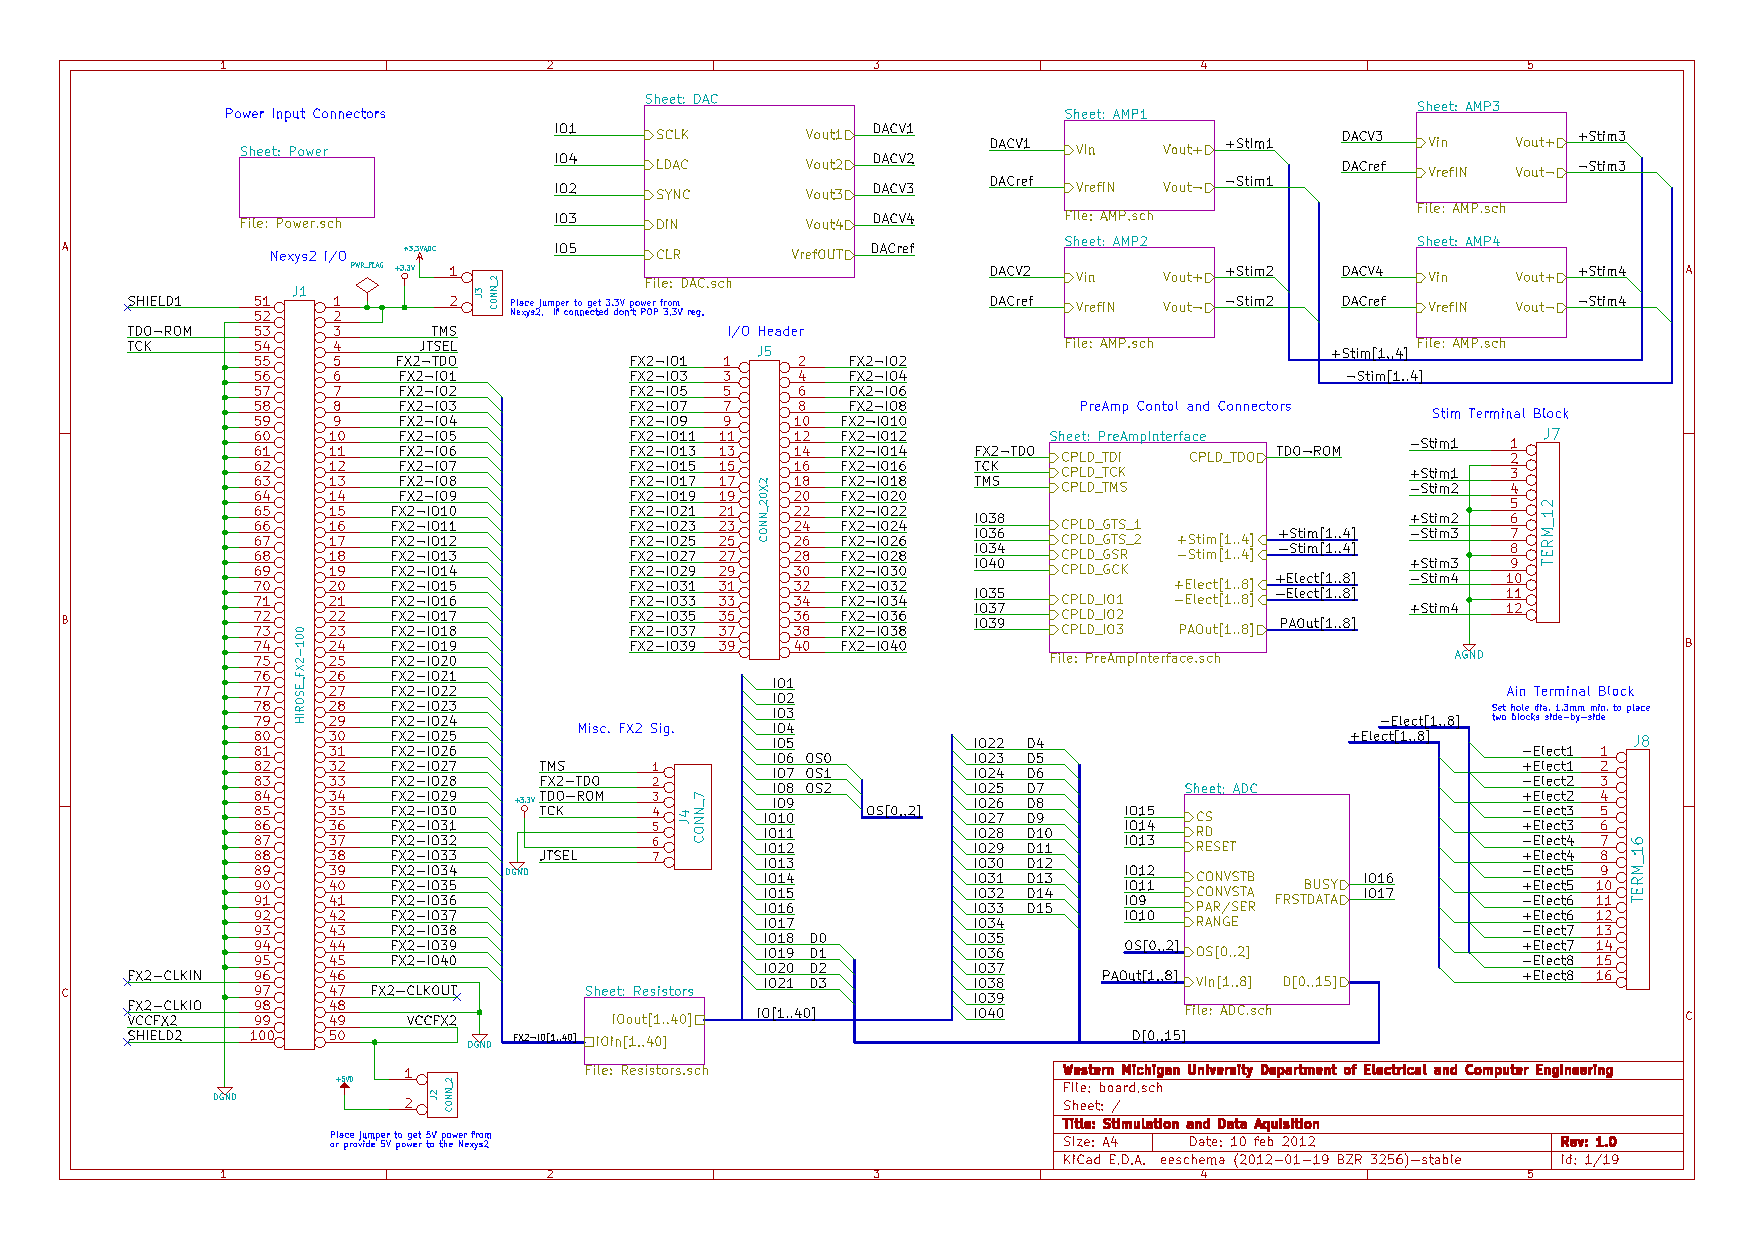
\includegraphics[page=1,trim=6.4in 3.7in 2.6in 2.8in,clip]{./figures/SchematicRev1r0} %[trim=left bottom right top]
	\caption{Example of a hierarchical block used to add sheets to the schematic\label{fig:hblock}}
	\end{singlespace}
\end{figure}

Local net labels, such as TCK on the root sheet, connect signals with the same net label without the need to draw a wire but are only valid on the same sheet.  Any signal labeled TCK on another sheet will not be connected the net on the root sheet.  To connect signals between sheets, hierarchical labels may be included on the sheet.  A hierarchical label, such as CPLD\_TCK on the PreAmpInterface sheet, is similar to a local net label in that its scope is only within the sheet but is special in that it can appear on the block symbol for the sheet.  Connecting a signal to the label on the block symbol connects the signal to the net designated by the hierarchical label, such as the TCK net on the root sheet connecting to the CPLD\_TCK net on the PreAmpInterface sheet by virtue of the connection of TCK to CPLD\_TCK on the block shown in Figure~\ref{fig:hblock}.

Hierarchical blocks can be called from any sheet in the hierarchy, not just the root sheet, which allows for multi-level hierarchies.  Figure~\ref{fig:hierarchy} shows the hierarchical structure of the Electrophysiology Interface board schematic.  Most blocks are called from the root sheet with the exception of the PreAmpInterface sheet, which itself calls several blocks.

\begin{figure}[h]
	\begin{singlespace}
	\centering
	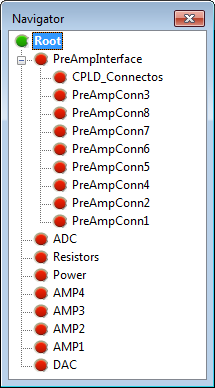
\includegraphics[width=1.5in]{./figures/Hierarchy}
	\caption{Sheet hierarchy in the Electrophysiology Interface board schematic \label{fig:hierarchy}}
	\end{singlespace}
\end{figure}

One of the advantages of hierarchical blocks is that, when parts of the circuit need to be replicated, such as in the case of the Differential Output Amplifier described in section~\ref{sec:DOA}, only one iteration of the circuit needs to be drawn.  Multiple hierarchical block symbols can reference a single schematic file.  Any changes to the circuit in one sheet will propagate to the other sheets whose blocks reference the same schematic file.  Figure~\ref{fig:hblockx4} shows how one schematic file is referenced by multiple blocks to allow four Differential Output Amplifier circuit blocks to be included in the schematic while only being drawn once.

\begin{figure}[h]
	\begin{singlespace}
	\centering
	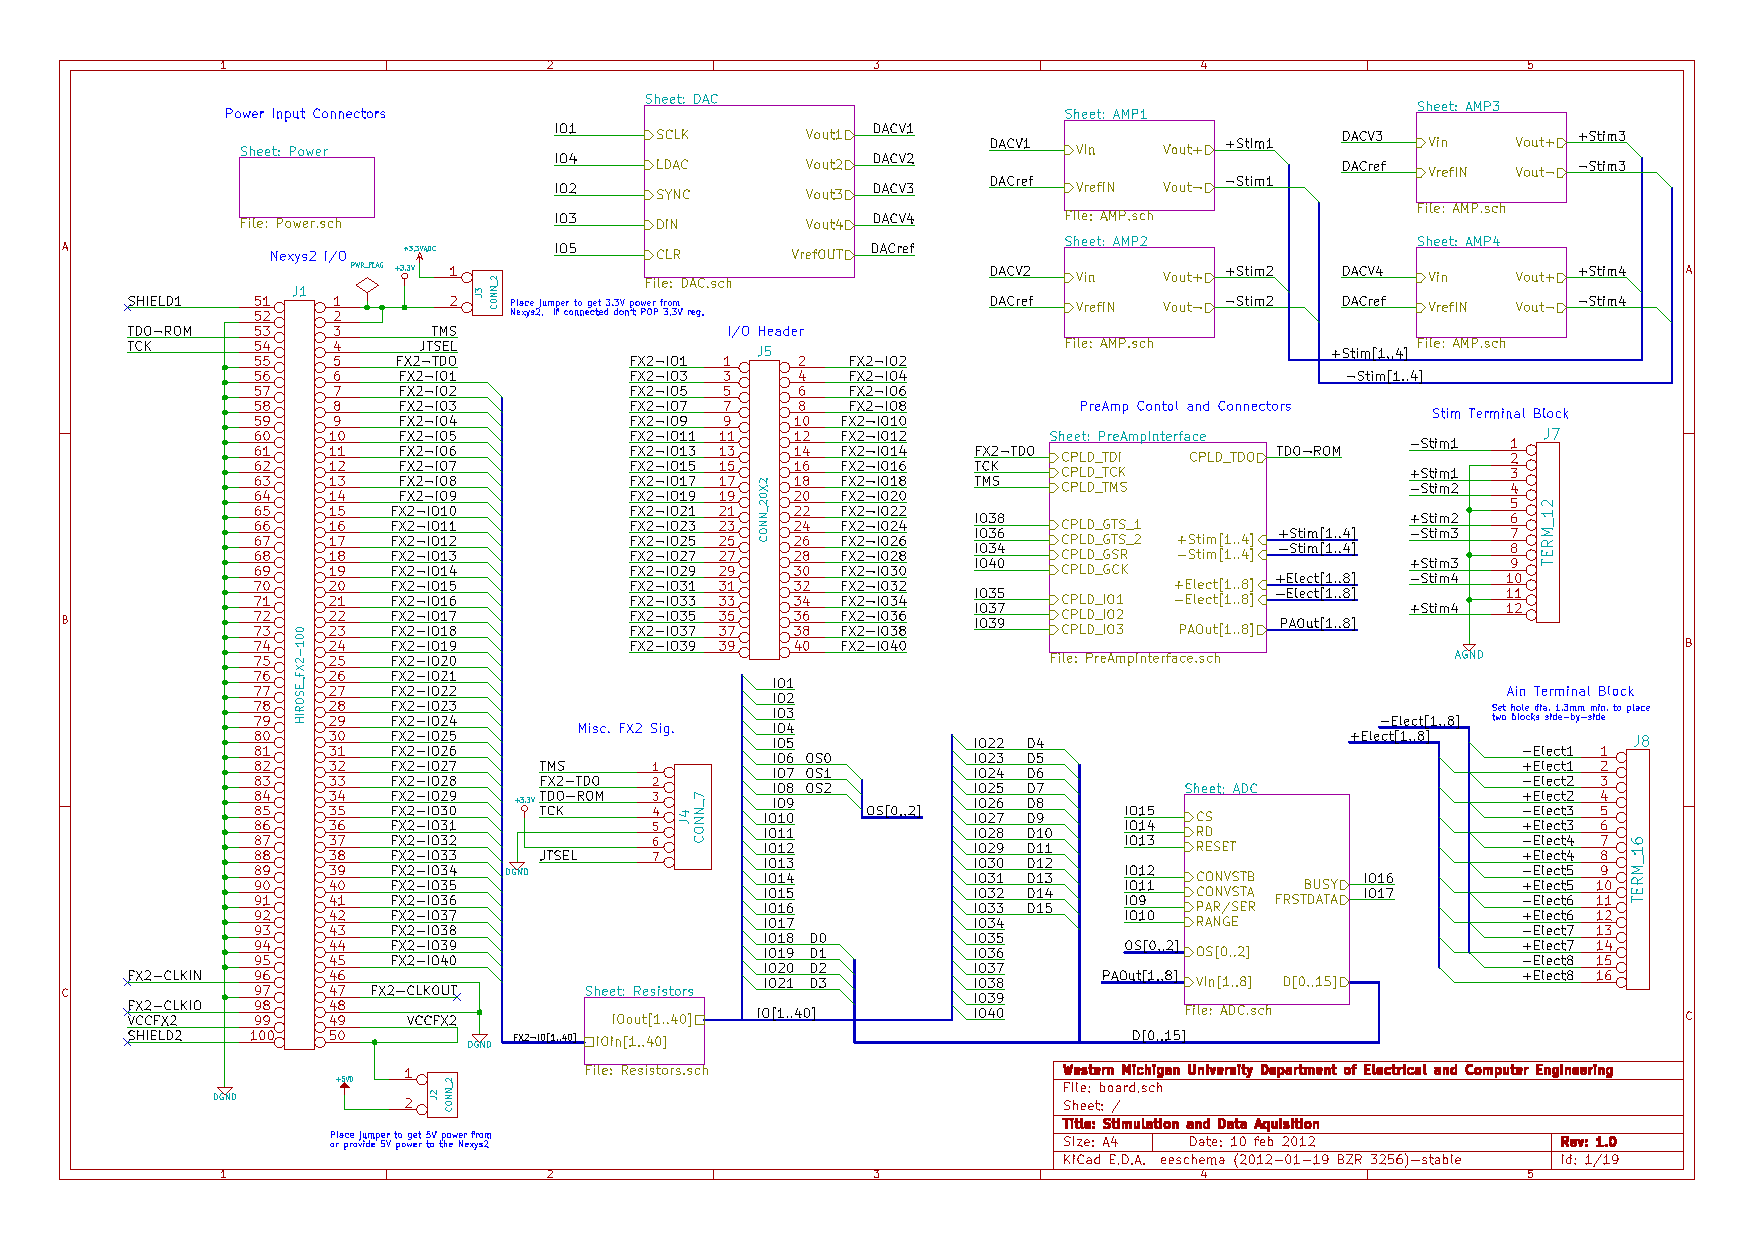
\includegraphics[page=1,trim=6.5in 5.6in 0.5in 0.6in,clip]{./figures/SchematicRev1r0} %[trim=left bottom right top]
	\caption{An example of four hierarchical blocks being used to replicate a single circuit design \label{fig:hblockx4}}
	\end{singlespace}
\end{figure}

The sheets AMP4 down to AMP1 on pages~\pageref{SchematicRev1r0.15} to~\pageref{SchematicRev1r0.18} are nearly identical, but it should be noted that the reference designators of the components on each sheet are unique.  For instance, the decoupling capacitors on sheet AMP1 are labeled C24 and C25 while the decoupling capacitors on sheet AMP2 are labeled C22 and C23.  Changing a reference designator on one sheet will not affect the other sheets, but adding or deleting components or drawing wires on one sheet will propagate to the other sheets.

Multiple component symbols are custom made for the Electrophysiology Interface board.  Most are based on symbols from KiCad symbol library and the information contained in the respective parts data sheets.  The Preamp PCI-Express connector symbol is based on a library from~\cite{osheclib}.  All custom component library files are stored in the $lib$ directory under the project directory to facilitate project portability between installations of KiCad.

Test points are included for most signals to facillitate rework and voltage measurement, with the exception of the CPLD and FPGA IO pins and JTAG signals, which are connected to header components.


\subsection{Component Footprint Selection}

The next step in designing the PCB in the KiCad EDA suite is to assign layout footprints to the components included in the schematic with the program CvPcb, which reads the netlist file created by Eeschema.  Through-hole footprints are utilized for connectors, protection diodes, and electrolytic capacitors.  Surface mount footprints are utilized for all other components to limit footprint size and lead length inductance~\cite{Montrose1999}.

Solder mount through-hole footprints with $0.1\unit{in}$ ($2.54\unit{mm}$) spacing are used for connectors with the exception of the Hirose FX2 and PCI-Express connectors.  Resistors, ceramic capacitors, and LEDs use standard 0805 package outline footprints as a compromise between choosing a package that minimizes the board space requirement and one that is large enough to be easy to solder by hand.  Small-Outline (SO) variations of integrated circuits are preferred when available for the component, and Quad-Flat Package (QFP) variations are used for the 64-pin count components.  Test points are implemented with a square pad of plated copper which minimizes required area on the board while allowing a test probe to connect to the signal and provides an acceptable surface for soldering a wire if rework is needed.

Custom footprints not included in the KiCad suite are used for several components and are included in the $lib$ directory under the main project directory.  The footprints for the Preamp PCI-Express connector and the CPLD are based on libraries from~\cite{osheclib}, and the footprint for the 100-pin Hirose FX2 connector is based on a library from~\cite{CodingAdvFX2}.  The footprint for the 16-pin terminal block for connecting to the recording electrodes was modified with a larger hole size to enable two 8-pin terminal blocks to be used side-by-side~\cite{TETermBlockDraw}.  Guide holes were modified to be plated to be compatible with the design constraints of the manufacturer~\cite{AdvCir66}.  All component footprints were compared to the recommended PCB footprints in the components' respective data sheets to ensure compatibility.

CvPcb saves the footprint information to the netlist file created by Eeschema.  The name for the footprints of each component can be seen in the $Package$ column on the bill of materials in Table~\ref{tab:bom} in Appendix~\ref{sec:bom}.

\subsection{Layout Overview}

%Description of the placement of the circuit blocks on the board
The next step in designing a PCB is creating the layout with the program Pcbnew included in the KiCad EDA suite.  The following work order is used when designing the layout of the PCB:

\paragraph{Setup PCB layers}

The top and bottom layers are used for signal routing; the inner layer near the top side is used for analog and digital ground planes; and the inner layer near the bottom side is used for analog and digital power planes.

\paragraph{Setup design constraints}
	
Design rules in Pcbnew are set to comply with the manufacturer design constraints in~\cite{AdvCir66} and~\cite{AdvCirTol}. Default trace widths are set to $0.008\unit{in}$ with $0.016\unit{in}$ width for power traces on the signal layers, and to save board area, the via drill size is set to the minimum $0.015\unit{in}$~\cite{AdvCir66}.  Blind and buried vias are not allowed~\cite{AdvCir66}.
	
\paragraph{Import netlist}

Pcbnew imports the netlist file created by Eeschema and CvPcb and places all of the component footprints in the layout window with vector lines representing connections between pins, creating the ``rats nest''~\cite{PcbnewRefMan}.

\paragraph{Draw PCB outline}

The board outline is drawn as a $4.75\unit{in}$ square, which matches the dimensions of the RTSC board.  

\paragraph{Place connectors}

Placement of the Hirose FX2 connector is critical to ensure proper mating with the connector on the RTSC board, and the PCI-Express connectors are placed close to the recording electrode terminal block the keep the trace length short.
	
\paragraph{Place remaining components}

The remaining components are placed on the top layer with some exceptions for resistors and capacitors.  Analog and digital components are placed while being mindful of the need to keep them above the analog and digital ground planes, respectively, without overlap.  Decoupling and Bypass capacitors are placed as close as possible to power pins and connectors, preferring to place the capacitors on the same side as the component.

\paragraph{Draw ground and power planes}

The power and ground planes are drawn on the inner layers in shapes that preserve analog and digital isolation and minimize trace length to the power and ground pins of components.  Figures~\ref{fig:PCBGND} and~\ref{fig:PCBPWR} show the ground and power planes, respectively, of the Electrophysiology Interface board.  Care must be taken to ensure that the copper planes maintain the minimum clearance around component and via holes ($0.010\unit{in}$ for inner layers) and the PCB edge ($0.015\unit{in}$ for inner layers) while also ensuring that the plane is continuous~\cite{AdvCirTol}.  Figure~\ref{fig:vitalclear} shows two locations on the power and ground layers where the plane clearance is vital to maintaining continuous planes.

Figure~\ref{fig:vitalPWR} shows where the +VA plane has a through-hole connector occupying the full height of the plane.  If the clearance between the plane and the hole features is too large, the plane will not be filled between the holes, disconnecting parts of the plane.  Likewise, in Figure~\ref{fig:vitalGND}, many pins on the two rows closest to the board edge need to connect to the DGND net; a large plane clearance will cut off the pins from the ground plane.

\begin{figure}[h]
	\begin{singlespace}
	\centering	
		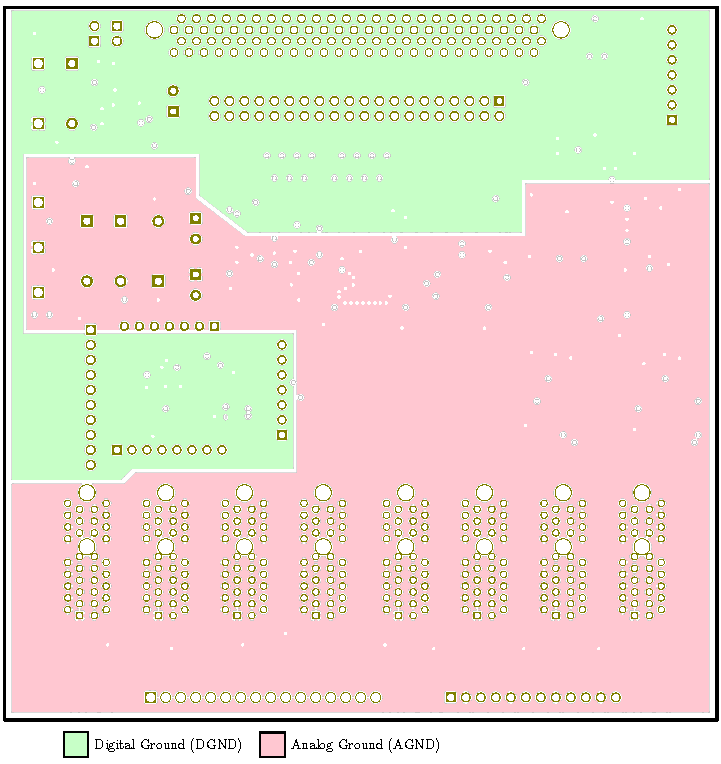
\includegraphics{./figures/PCBCopperGND} 
	\caption{PCB ground plane layer\label{fig:PCBGND}}
	\end{singlespace}
\end{figure}

\begin{figure}[h]
	\begin{singlespace}
	\centering 
		\includegraphics{./figures/PCBCopperPWR} 
	\caption{PCB power plane layer\label{fig:PCBPWR}}
	\end{singlespace}
\end{figure}

\begin{figure}[h]
	\centering 
	\begin{singlespace}
	\begin{subfigure}[b]{0.35\textwidth}
		\centering 
		\includegraphics[trim=1in 1.25in 3in 3.5in,clip,width=\textwidth]{./figures/PCBCopperPWR} %[trim=left bottom right top]
	\caption{Power plane\label{fig:vitalPWR}}
	\end{subfigure}
	~
	\begin{subfigure}[b]{0.35\textwidth}
		\centering 
		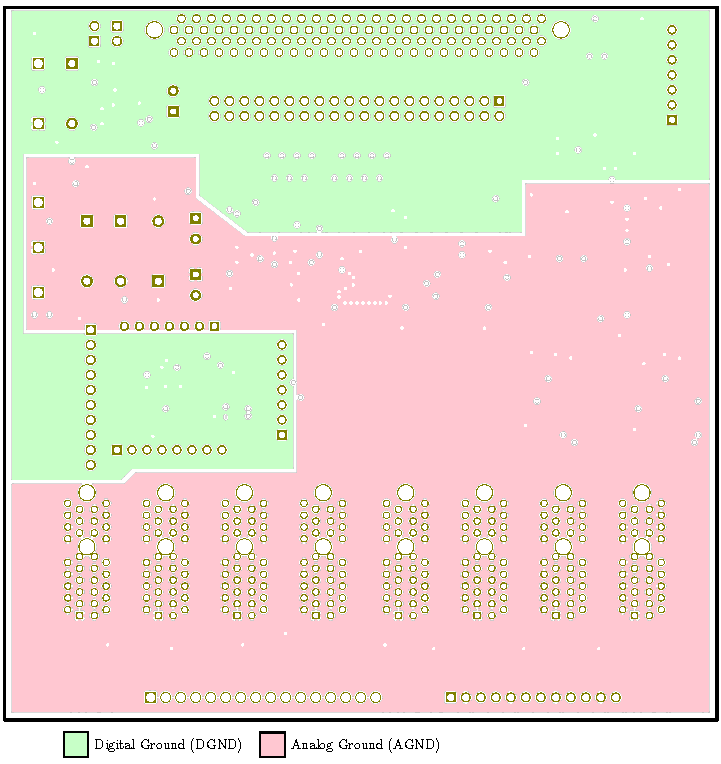
\includegraphics[trim=0.9in 4.7in 3.25in 0in,clip,width=\textwidth]{./figures/PCBCopperGND} %[trim=left bottom right top]
	\caption{Ground plane\label{fig:vitalGND}}
	\end{subfigure}
	\caption{Close clearances on power and ground planes\label{fig:vitalclear}}
	\end{singlespace}
\end{figure}

\paragraph{Route critical signal traces}

The signals most susceptible to signal integrity issues should be routed first.  These signals include the high-frequency digital signals between the FPGA, ADC, and DAC and the noise susceptible signal from the recording electrodes.  The traces should be routed with minimum length, through as few vias as possible, and on the layer adjacent to the ground plane~\cite{Montrose1999}.

\paragraph{Route remaining traces}

After the components are placed, ground planes drawn, and susceptible traces routed, the remaining signal traces may be routed.  To avoid disfigurement of the trace during the etching process, narrow traces are routed so that they never form a right angle: they first turn $45^\circ$, then they extend at least a short distance, and finally they can make another $45^\circ$ turn~\cite{ExpresssPCBTips}.  Figure~\ref{fig:PCBTopBot} shows the traces and pads on the top and bottom layers of the PCB.

\begin{figure}[htb]
	\begin{singlespace}
	\centering 
		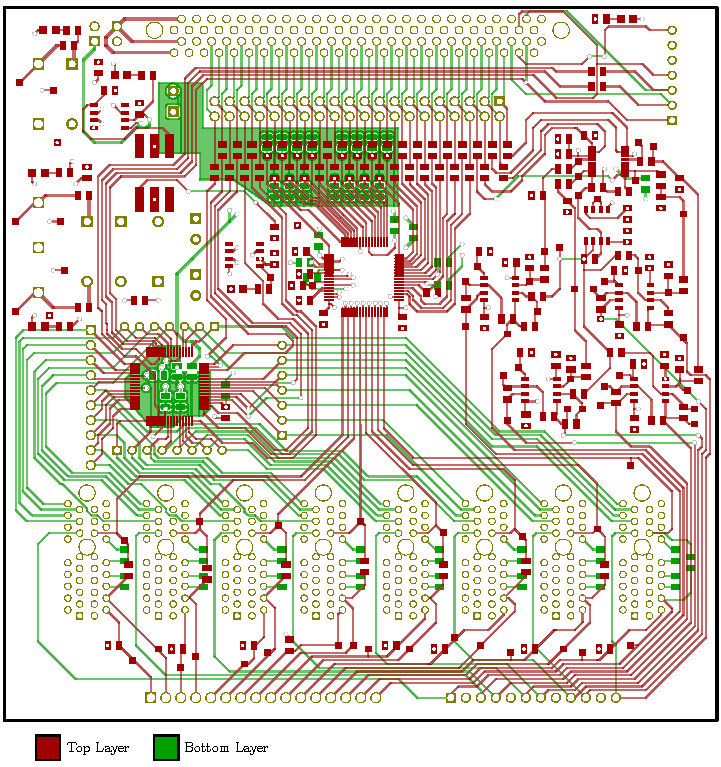
\includegraphics{./figures/PCBCopperTopBot} 
	\caption{PCB top and bottom signal layers\label{fig:PCBTopBot}}
	\end{singlespace}
\end{figure}
	
\paragraph{Place test points}

After the traces are routed is the best time to place the test points on the board.  The placement of the test point pads is not critical for the Electrophysiology Interface board, but the size of the pad can interfere with trace routing; thus, the test points can be located last.  The test point pads should be placed so as to be accessible after the components are populated.
	
\paragraph{Iterate this procedure as needed based on signal routing}

To adapt to the challenges encountered during signal routing, it is necessary to adjust ground and power planes, move components, edit component footprints, and change signal connections on the schematic.  For instance, the CPLD connections to the Preamp connectors are entirely based on the routing needs of the board layout.

\paragraph{Move labels on the silkscreen layer}

Finally, after all the signals are successfully routed, the reference designators for the individual components should be moved so that the labels are visible after the parts are populated on the board, allowing physical parts to be matched to the components in the schematic.  Labels should not be located under parts or on top of exposed copper pads.





\subsection{Manufacturing and Assembly}

To produce a PCB, the layout design is transmitted to a manufacturer and a finished PCB is shipped.  The standard method of sharing layout design files between the designer and manufacturer is the text-based Gerber and Excellon drill file formats.  Still, there are enough variations in file naming, packaging, number format, and drill files that the manufacturer's requirements and EDA suite capabilities need to be carefully scrutinized.  Advanced Circuits is capable of receiving Gerber files in the newer 247X format, Excellon drill files, and Gerber FAB files~\cite{AdvCirFile, AdvCirGerMis, AdvCirFreeDFMCheck}.  The company also offers an automated Gerber file review and quoting service that can increase confidence in the successful manufacturing of the PCB design~\cite{AdvCirFreeDFMCheck}.  The procedure for creating the design files required for the Advanced Circuits manufacturing services is elucidated in Appendix~\ref{sec:gerberexp}.

A PCB is useless without components with which to populate the board.  Table~\ref{tab:bom} in Appendix~\ref{sec:bom} shows the bill of materials required to populate the Electrophysiology Interface board.  Components may be ordered from electronics supplier DigiKey\textsuperscript{\textregistered}, and the table includes the supplier part numbers and prices as of March 2013.  Components for the Electrophysiology Interface board are sourced from DigiKey\textsuperscript{\textregistered} along with samples provided by Analog Devices\textsuperscript{\textregistered} and Linear Technology\textsuperscript{\textregistered}.

After the PCB and components are received, assembly is required.  Components are populated by soldering them to the board by hand.  Logical circuit blocks, as defined in the subsections of section~\ref{sec:hardware}, are populated together while constantly testing for unintended short and open circuit conditions by using a resistance meter and by powering the board after each logical block is populated.  Soldering the most difficult components of the logical block first, such as ICs, is a good strategy to allow the best possible access to the hard to see and reach pins.  Pictures of the assembled Electrophysiology Interface board can be seen in Figures~\ref{fig:eitop} and~\ref{fig:eibot}.

\begin{figure}[H]
	\begin{singlespace}
	\centering	
		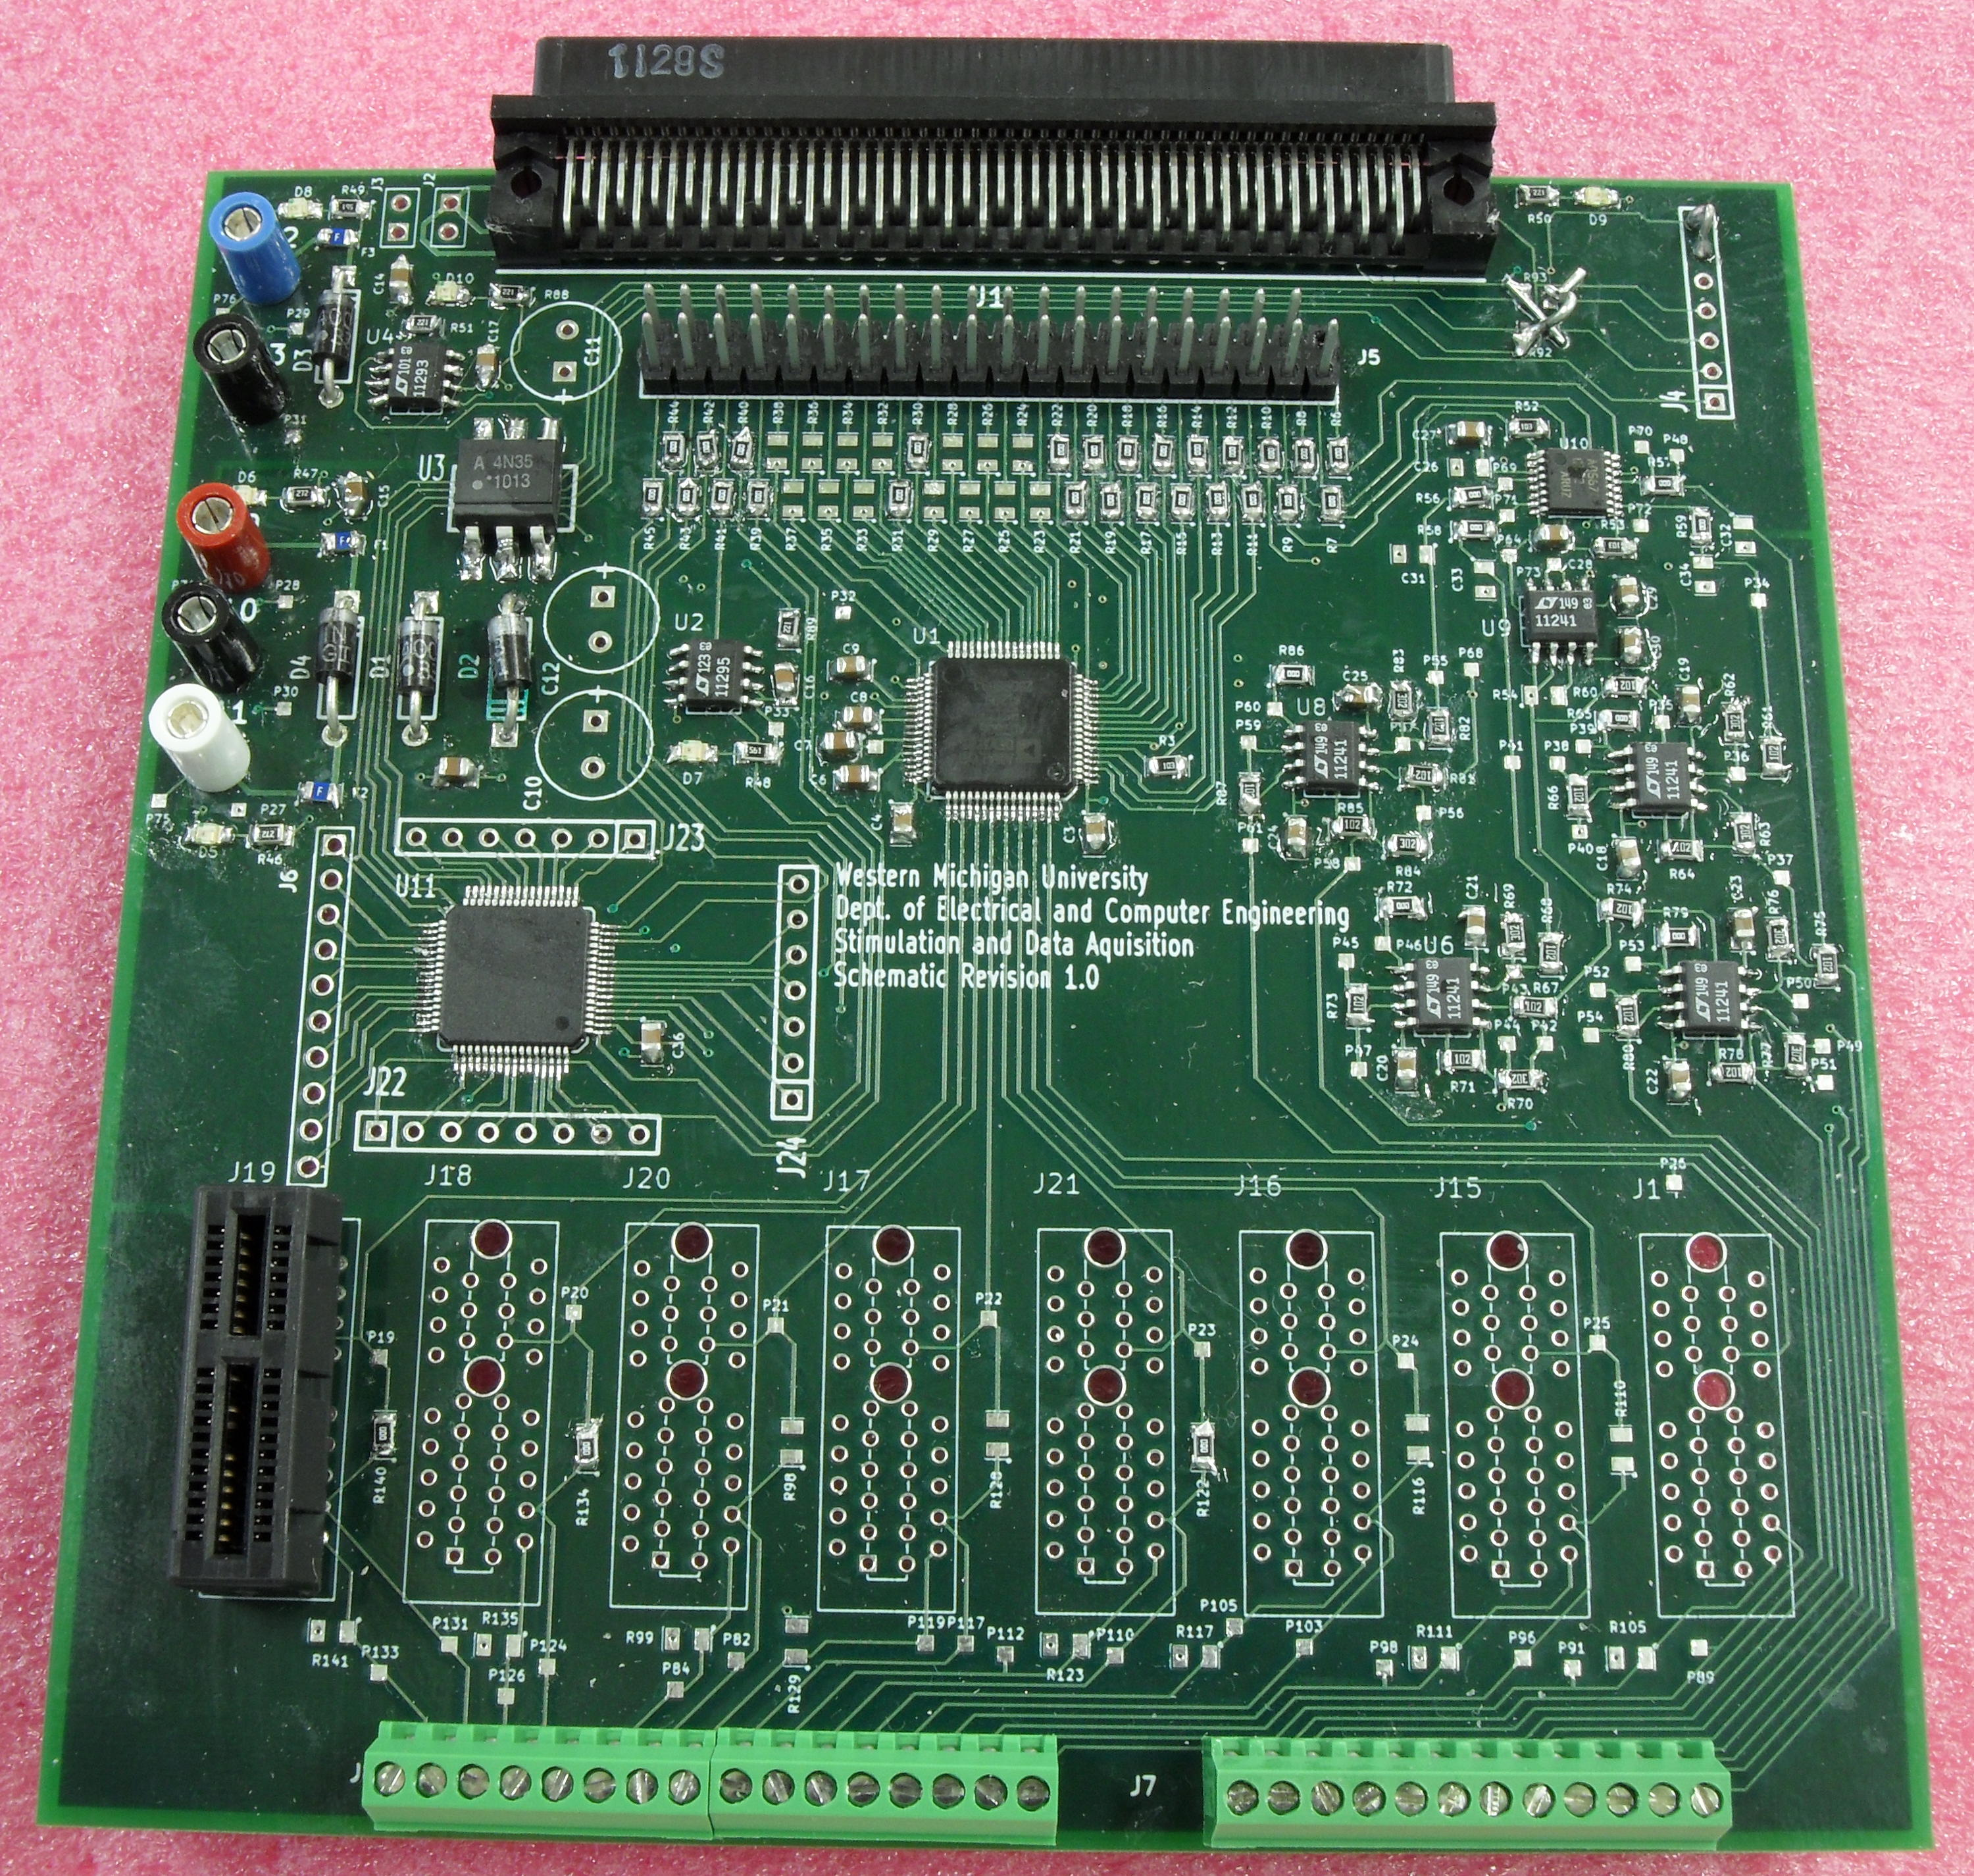
\includegraphics{./figures/EITop} 
	\caption{View of the top side of the populated Electrophysiology Interface board\label{fig:eitop}}
	\end{singlespace}
\end{figure}

\begin{figure}[H]
	\begin{singlespace}
	\centering	
		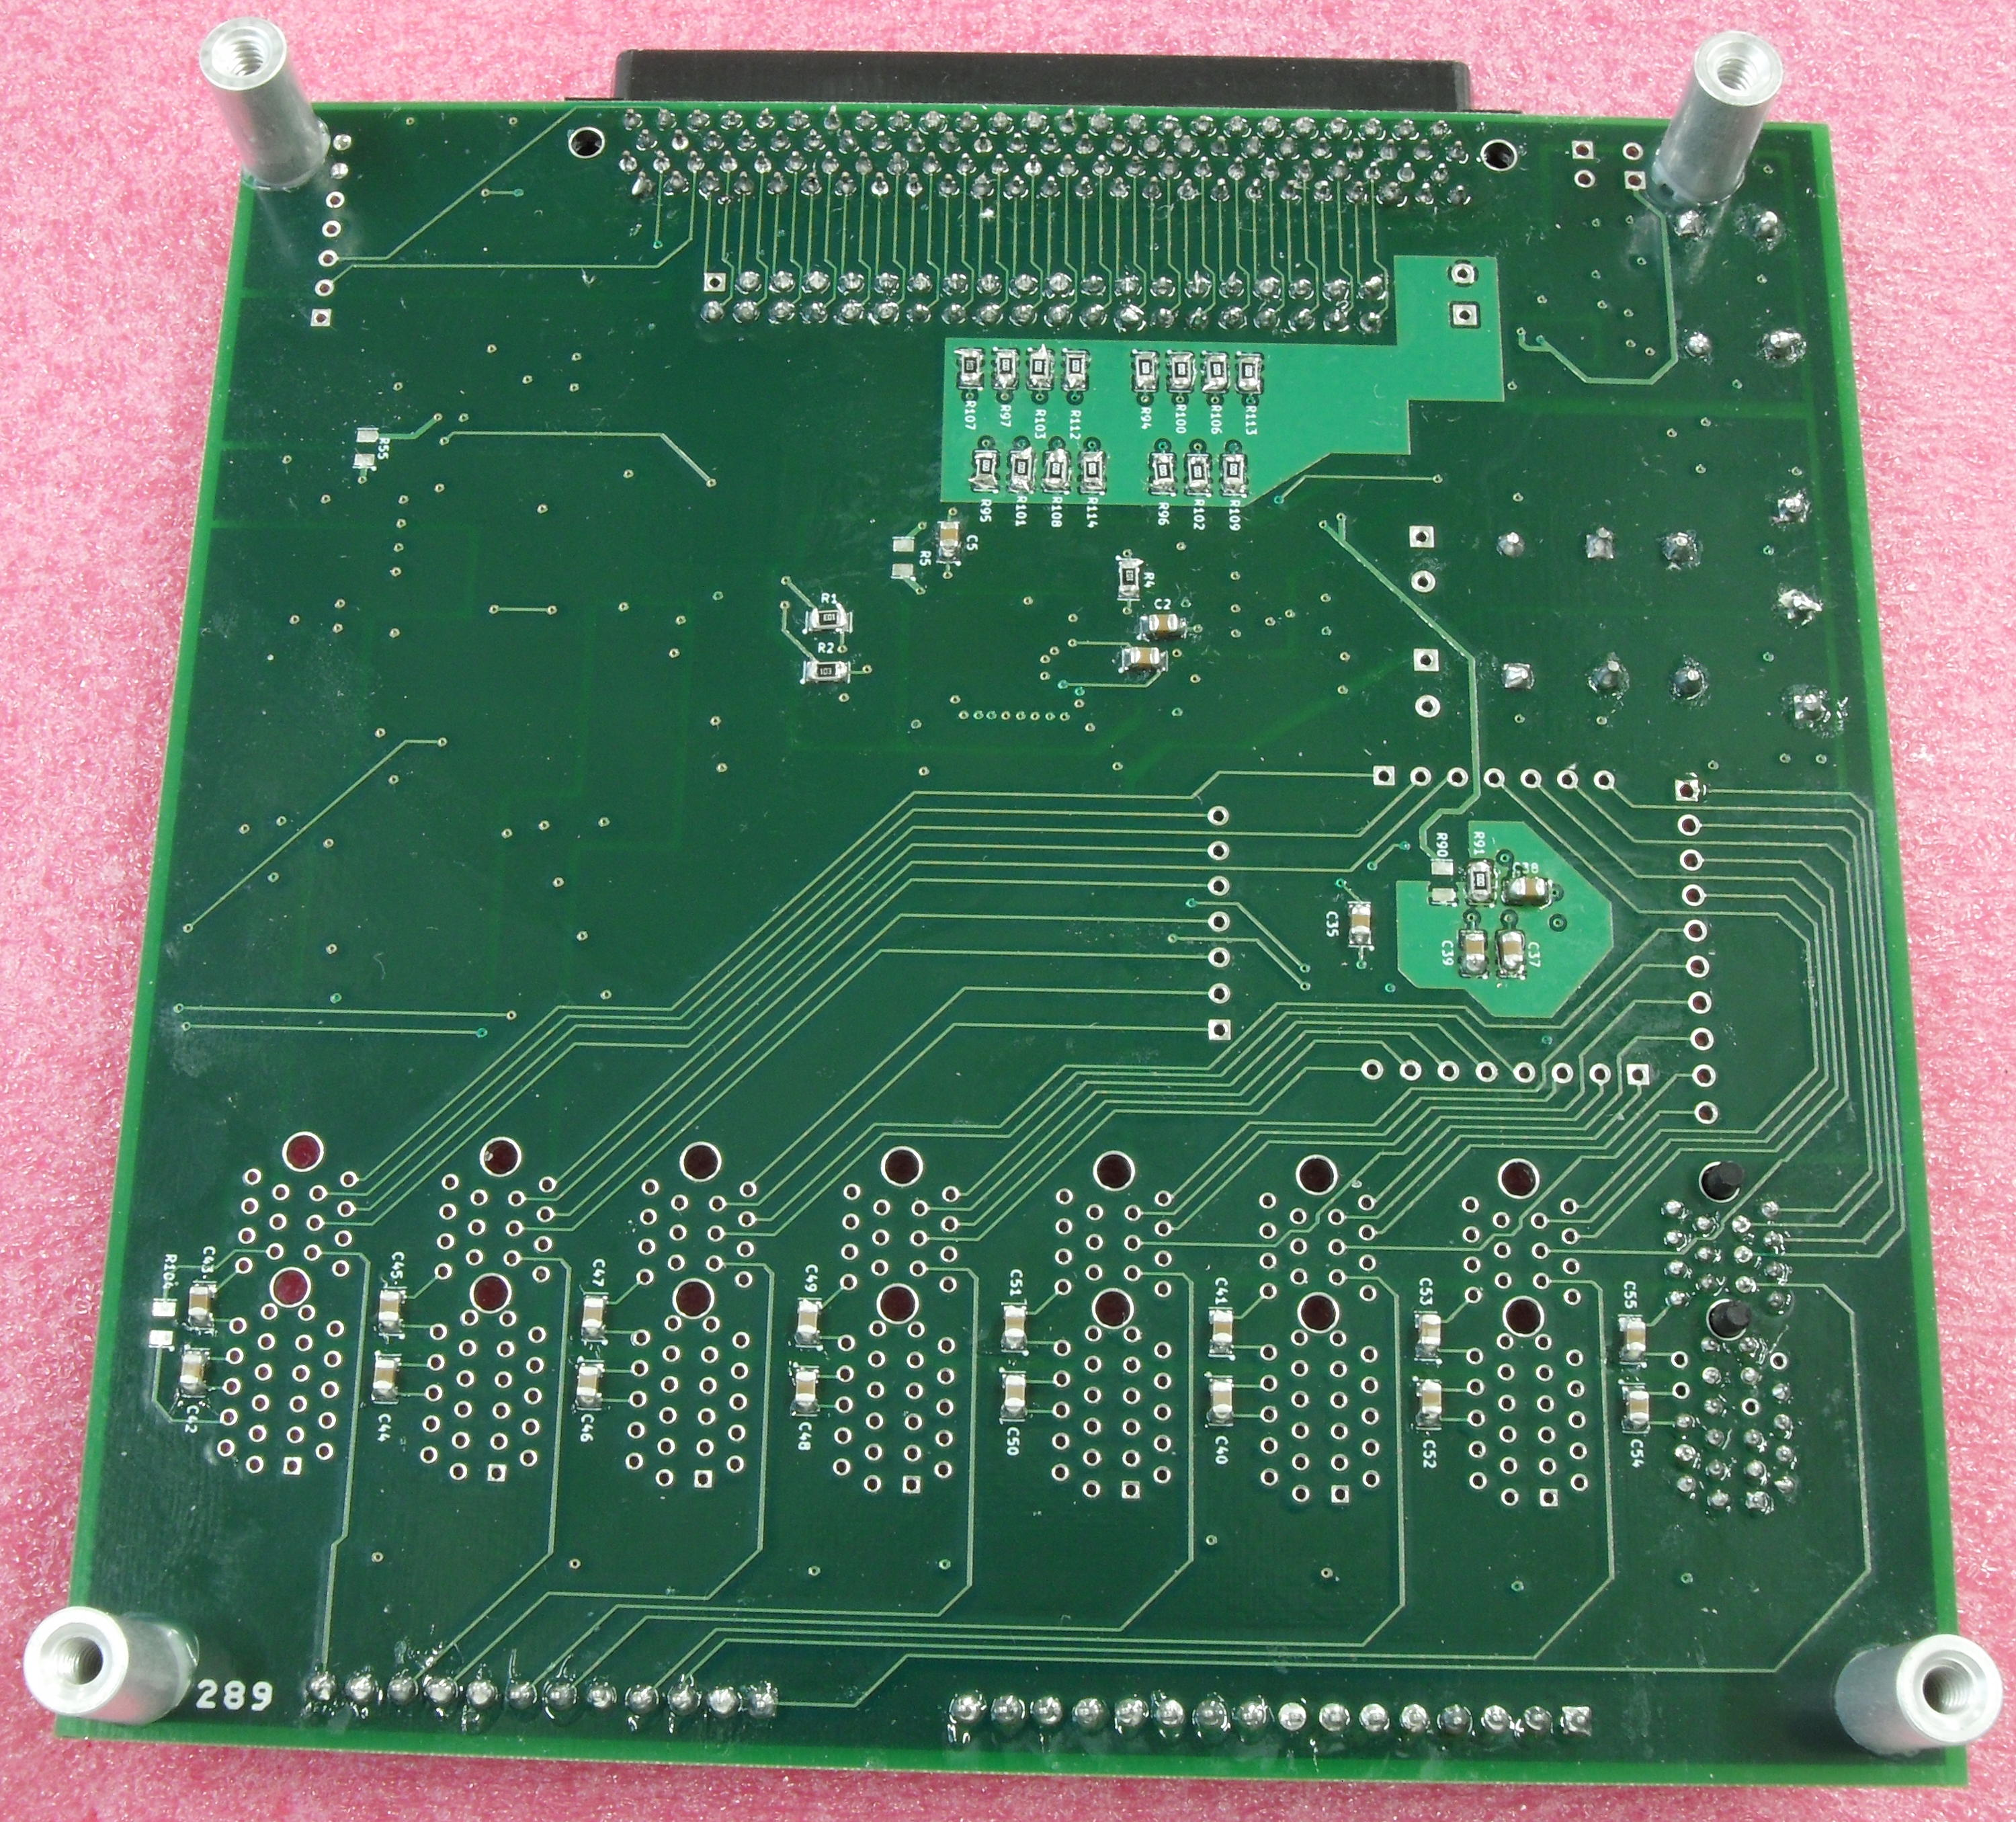
\includegraphics{./figures/EIBot} 
	\caption{View of the bottom side of the populated Electrophysiology Interface board\label{fig:eibot}}
	\end{singlespace}
\end{figure}


\section[Electrophysiology Application]{Electrophysiology Application\footnote{This section is co-authored with Kyle Batzer,~\cite{BatzerMSEE}.}}\label{sec:app}

%Description of the experiment performed to verify that the system can work with bio-electrical signals results also in earthworm.tex
%\subsection{System Validation}

To validate the stimulation and data acquisition system design, a standard electrophysiology experiment, described in~\cite{Olivo,KuehJellies,EllingerMSEE}, was performed on earthworm giant axon action potentials, henceforth referred to as the Earthworm Experiment.  This serves the purpose of showing that the Data Acquisition and Stimulation System is capable of being used in an electrophysiology experiment, and the procedure has been performed with previous designs, allowing the new design to be compared with previous results~\cite{StahlMSEE}.

%The earthworm's nerve fibers do not have a myelin sheath like many larger animals.  A myelin sheath insulates the ionic solution outside of the nerve fiber and results in faster propagation of an electric potential along the length of the fiber.  Without the myelin sheath the earthworm can not quickly propagate instructions to its muscles, which inhibit its response to dangers in its environment.  To overcome this limitation, there are giant axons along its nerve cord that are bundles of nerve fibers that each transmit the same information.  This arrangement results in faster propagation of the electric potential allowing the earthworm to quickly respond to danger.

In the earthworm's nerve cord, there is a median giant axon and two smaller lateral giant axons on either side of the median axon.  The lateral giants are connected to each other at multiple locations along the length of the earthworm which has the effect of lateral axons acting as a single giant axon~\cite{Olivo}.  A physical or electrical stimulation near the anterior or posterior ends of the earthworm will elicit a response from the earthworm in the form of an action potential that propagates along one or both of the giant axons.  The propagation speed is related to the cross sectional area of the axon~\cite{KuehJellies}.  Varying the intensity of the electrical stimulation at the anterior end of the earthworm will show no response at low intensity, an action potential along the median axon soon after the stimulation at medium intensity, and at a higher intensity, action potentials along both the median and lateral giant axons will be visible with the median response occurring sooner than the lateral response due to the differing propagation speeds.  Figure~\ref{fig:EWCrossSec} shows a cross section of an earthworm based on a figure in~\cite{Kladt2010} with a more detailed representation of the nerve cord based on~\cite{KuehJellies}.

\begin{figure}[H]
	\begin{singlespace}
	\centering 
		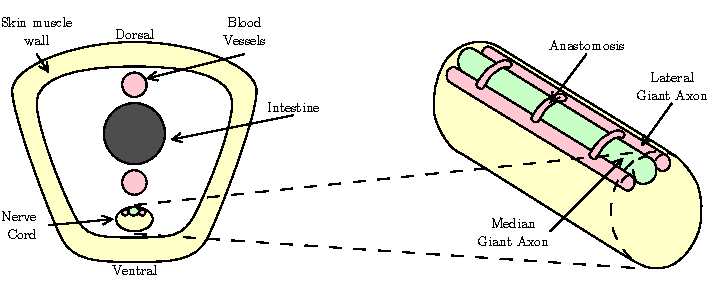
\includegraphics{./figures/EWCrossSec} 
	\caption{Cross section of an earthworm adapted from~\cite{KuehJellies,Kladt2010}\label{fig:EWCrossSec}}
	\end{singlespace}
\end{figure}


Electrical stimulation is accomplished by placing two pins near the anterior end of the earthworm.  Measurement of the action potentials along the axon is accomplished by dissecting the earthworm and placing two chlorided silver extracellular electrodes on the earthworm nerve cord.  The extracellular electrodes measure the difference in electric potential at two points on the nerve cord.  When an action potential propagates along the nerve cord, the electrodes measure a difference in voltage in time that will appear as a biphasic spike.  The exact shape of the spike will depend on the placement and size of the electrodes and the condition of the nerve cord itself~\cite{Olivo,KuehJellies,McGillCAP}.

The Data Acquisition and Stimulation System was used to perform an experiment studying earthworm giant axon action potentials with a previously developed and validated amplifier~\cite{StahlMSEE} and oscilloscope connected in parallel with the electrophysiology interface board, allowing the data to be compared.

\subsection{Earthworm Setup}

The dissection of the earthworm and setup of the stimulation and recording hardware is based on~\cite{Olivo,KuehJellies,StahlMSEE}.  Two pins are placed near the anterior end of the earthworm.  Connected to these pins is the output of the stimulation circuitry. Near the middle of the earthworm, the skin is cut and folded to expose the interior of the worm.  The intestine is moved out of the way, and the nerve cord is pulled away from the fluids with two chlorided silver electrodes that are connected to the amplification and recording circuitry. Between the stimulation pins and recording electrodes, a chlorided silver wire is placed under the body of the earthworm and connected to circuit ground, which may be connected to earth ground depending on the circuit setup.  Figure~\ref{fig:EWSetup} is a diagram of the DASS connected to the earthworm

\begin{figure}[H]
	\begin{singlespace}
	\centering 
		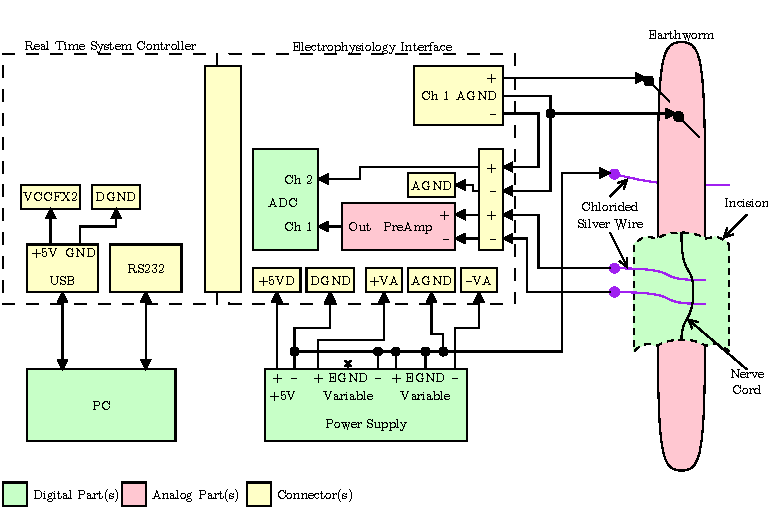
\includegraphics{./figures/EWSetup} 
	\caption{Diagram showing connections between the Data Acquisition and Stimulation System and an earthworm, connections to earthworm follow~\cite{Olivo,KuehJellies}\label{fig:EWSetup}}
	\end{singlespace}
\end{figure}

To compare the Data Acquisition and Stimulation System with a previously validated setup, the  Preamp from~\cite{StahlMSEE,BatzerCorsiCrampton}, with its output connected to an oscilloscope, has its input connected in parallel with the recording electrodes as shown in Figure~\ref{fig:EWSetupPA}.

\begin{figure}[H]
	\begin{singlespace}
	\centering 
		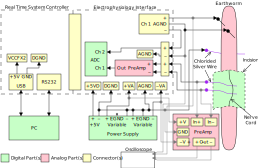
\includegraphics{./figures/EWSetupPA} 
	\caption{Diagram of the Data Acquisition and Stimulation System connected in parallel with a previously validated recording system, connections to the earthworm follow~\cite{Olivo,KuehJellies} and connections to the standalone Preamp and oscilloscope follow~\cite{StahlMSEE}\label{fig:EWSetupPA}}
	\end{singlespace}
\end{figure}

\subsection{Chloriding Silver Wire}

The silver wire used for the extracellular electrodes must be coated in a layer of silver chloride.  To create the coating, electroplating may be used as described in~\cite{KuehJellies,WarnerChloriding}. A simpler method is to place the portion of the wire that will be in contact with living tissue in full-strength Clorox\textsuperscript{\textregistered} bleach and leave the wire in the bleach until the wire acquires a purplish-gray tint, which should take between ten and thirty minutes~\cite{WarnerChloriding}.
 
\subsection{Earthworm Experiment Procedure}

The Earthworm Experiment procedure is adapted from~\cite{Olivo,KuehJellies}.

\subsubsection{Earthworm Dissection}

\begin{itemize}

\item Place the earthworm in a 10\% ethanol solution to anesthetize it

\item Leave the worm in the ethanol solution for the minimum amount of time needed to make the worm easy to work with while dissecting it; 5-10 minutes may be all that is necessary

\item Rinse the earthworm in tap water and pin it, dorsal (dark) side up, on the dissecting dish

\item Create a capital-letter-I shaped incision, using surgical scissors, one to two inches long, along the length of the worm, about halfway between the anterior and posterior ends of the earthworm

\item Pin the skin to the dissecting dish to expose the worm internal anatomy

\item Flush the cavity periodically, as needed, with worm Ringer's solution (in mM units: 102.7 NaCl, 1.6 KCl, 1.8 CaCl$_2$, and 4 NaHCO$_3$~\cite{KuehJellies}) to make the anatomy easier to view

\item Move the intestine aside, using forceps and scissors, exposing the nerve cord

\item Free a few centimeters of the nerve cord from its lateral and ventral connections, using the forceps and scissors, to allow the cord to be lifted above and away from the saline and other anatomy

\item Position the chlorided silver wires under the nerve cord

\item Raise the fixture holding the silver wires until the wires and nerve cord are away from the saline and earthworm anatomy (a fraction of an inch is all that is necessary, blowing in the area can break up the surface tension if the saline solution is bridging the wires and cord with the rest of the earthworm)

\item Moisten the nerve cord with Ringer's solution, often, throughout the experiment while making sure that the nerve cord and electrodes remain isolated from the rest of the saline and anatomy (it may be necessary to remove excess Ringer's solution)

\end{itemize}

\subsubsection{Electrical Setup}

\begin{itemize}

\item Place two pins near each other in the anterior end of the earthworm

\item Connect the non-inverting output of the stimulation circuit to one pin and connect circuit ground or the inverting output to the second pin

\item Connect, optionally, if the inverting output is not connected to a pin in the earthworm, the inverting output of the stimulation circuit to an unused electrode input channel on the Electrophysiology Interface board; ensure that there is no Preamp board in the PCI-Express socket and bypass the socket wiith a $0\Omega$ resistor.  See Figures~\ref{fig:EWSetup} and~\ref{fig:EWSetupPA}  

\item Place a chlorided silver wire under the body of the earthworm, between the stimulation pins and the exposed portion of the earthworm's body and connect the wire to circuit (which may be earth) ground

\item Connect the chlorided silver recording electrodes to the Preamp inputs with the non-inverting input connected toward the anterior end of the earthworm and the inverting input connector toward the posterior end (reversing the electrodes will simply invert the signal) (connecting the electrodes may be performed before the silver wires are placed under the nerve cord, to avoid disturbing the electrodes in the process of making the connections)

\item Power on the Electrophysiology Interface, first, then power on the RTSC

\end{itemize}

\subsubsection{Software Setup}

\begin{itemize}

\item Update FPGA program as described in~\cite{BatzerMSEE}

\item Update Cypress EZ-USB firmware as described in~\cite{BatzerMSEE}

\item Create the script and corresponding waveform file as shown in~\cite{BatzerMSEE}

\item Launch Data Acquisition and Stimulation Control Center (DASCC)

\item Select the appropriate COM port from the dropdown list

\item Select the appropriate Endpoint from the dropdown list, set Packets Per Xfer to 64, and set Xfers to Queue to 64

\item Select the Scripting tab and load the Earthworm Script as described in~\cite{BatzerMSEE}

\item When prepared for single stimulus and capture click the ``Run Script'' button.  Changes to the output pulse amplitude can be accomplished by changing the 2nd line of the Waveform file as shown in~\cite{BatzerMSEE}

\item Graph data by selecting the Graphing tab and clicking the ``Load File'' button.  Once loaded, multiple channels can be displayed at the same time using ctrl + left mouse button to select/deselect channels.

\item Click ``Output CSV'' to export data to a comma-separated values (CSV) text file

\end{itemize}

\subsubsection{Stimulation and Recording}

\begin{itemize}

\item Stimulate the earthworm with a single, $0.2\unit{ms}$ wide pulse with low amplitude (less than $1.0\unit{V}$)

\item Repeat the stimulation while slowly increasing the pulse amplitude (in steps between $0.1\unit{V}$ and $0.5\unit{V}$) until a response is seen between $2\unit{ms}$ and $8\unit{ms}$ after the stimulation artifact, this is the median giant response

\item Save the recorded waveform

\item Slowing increase the pulse amplitude, further, until a second response is seen between $6\unit{ms}$ and $15\unit{ms}$ after the stimulation artifact, this is the lateral giant response

\item Save the recorded waveform

\end{itemize}

\subsection{Results}\label{sec:results}

The Earthworm Experiment was performed with the Data Acquisition and Stimulation System connected in parallel with a preamp and oscilloscope that was validated in~\cite{StahlMSEE}.  A diagram of the experimental setup is shown in Figure~\ref{fig:EWSetupPA}.  A picture of the experimental setup is shown in Figure~\ref{fig:EWSetupPic}.

\begin{figure}[H]
	\begin{singlespace}
	\centering 
		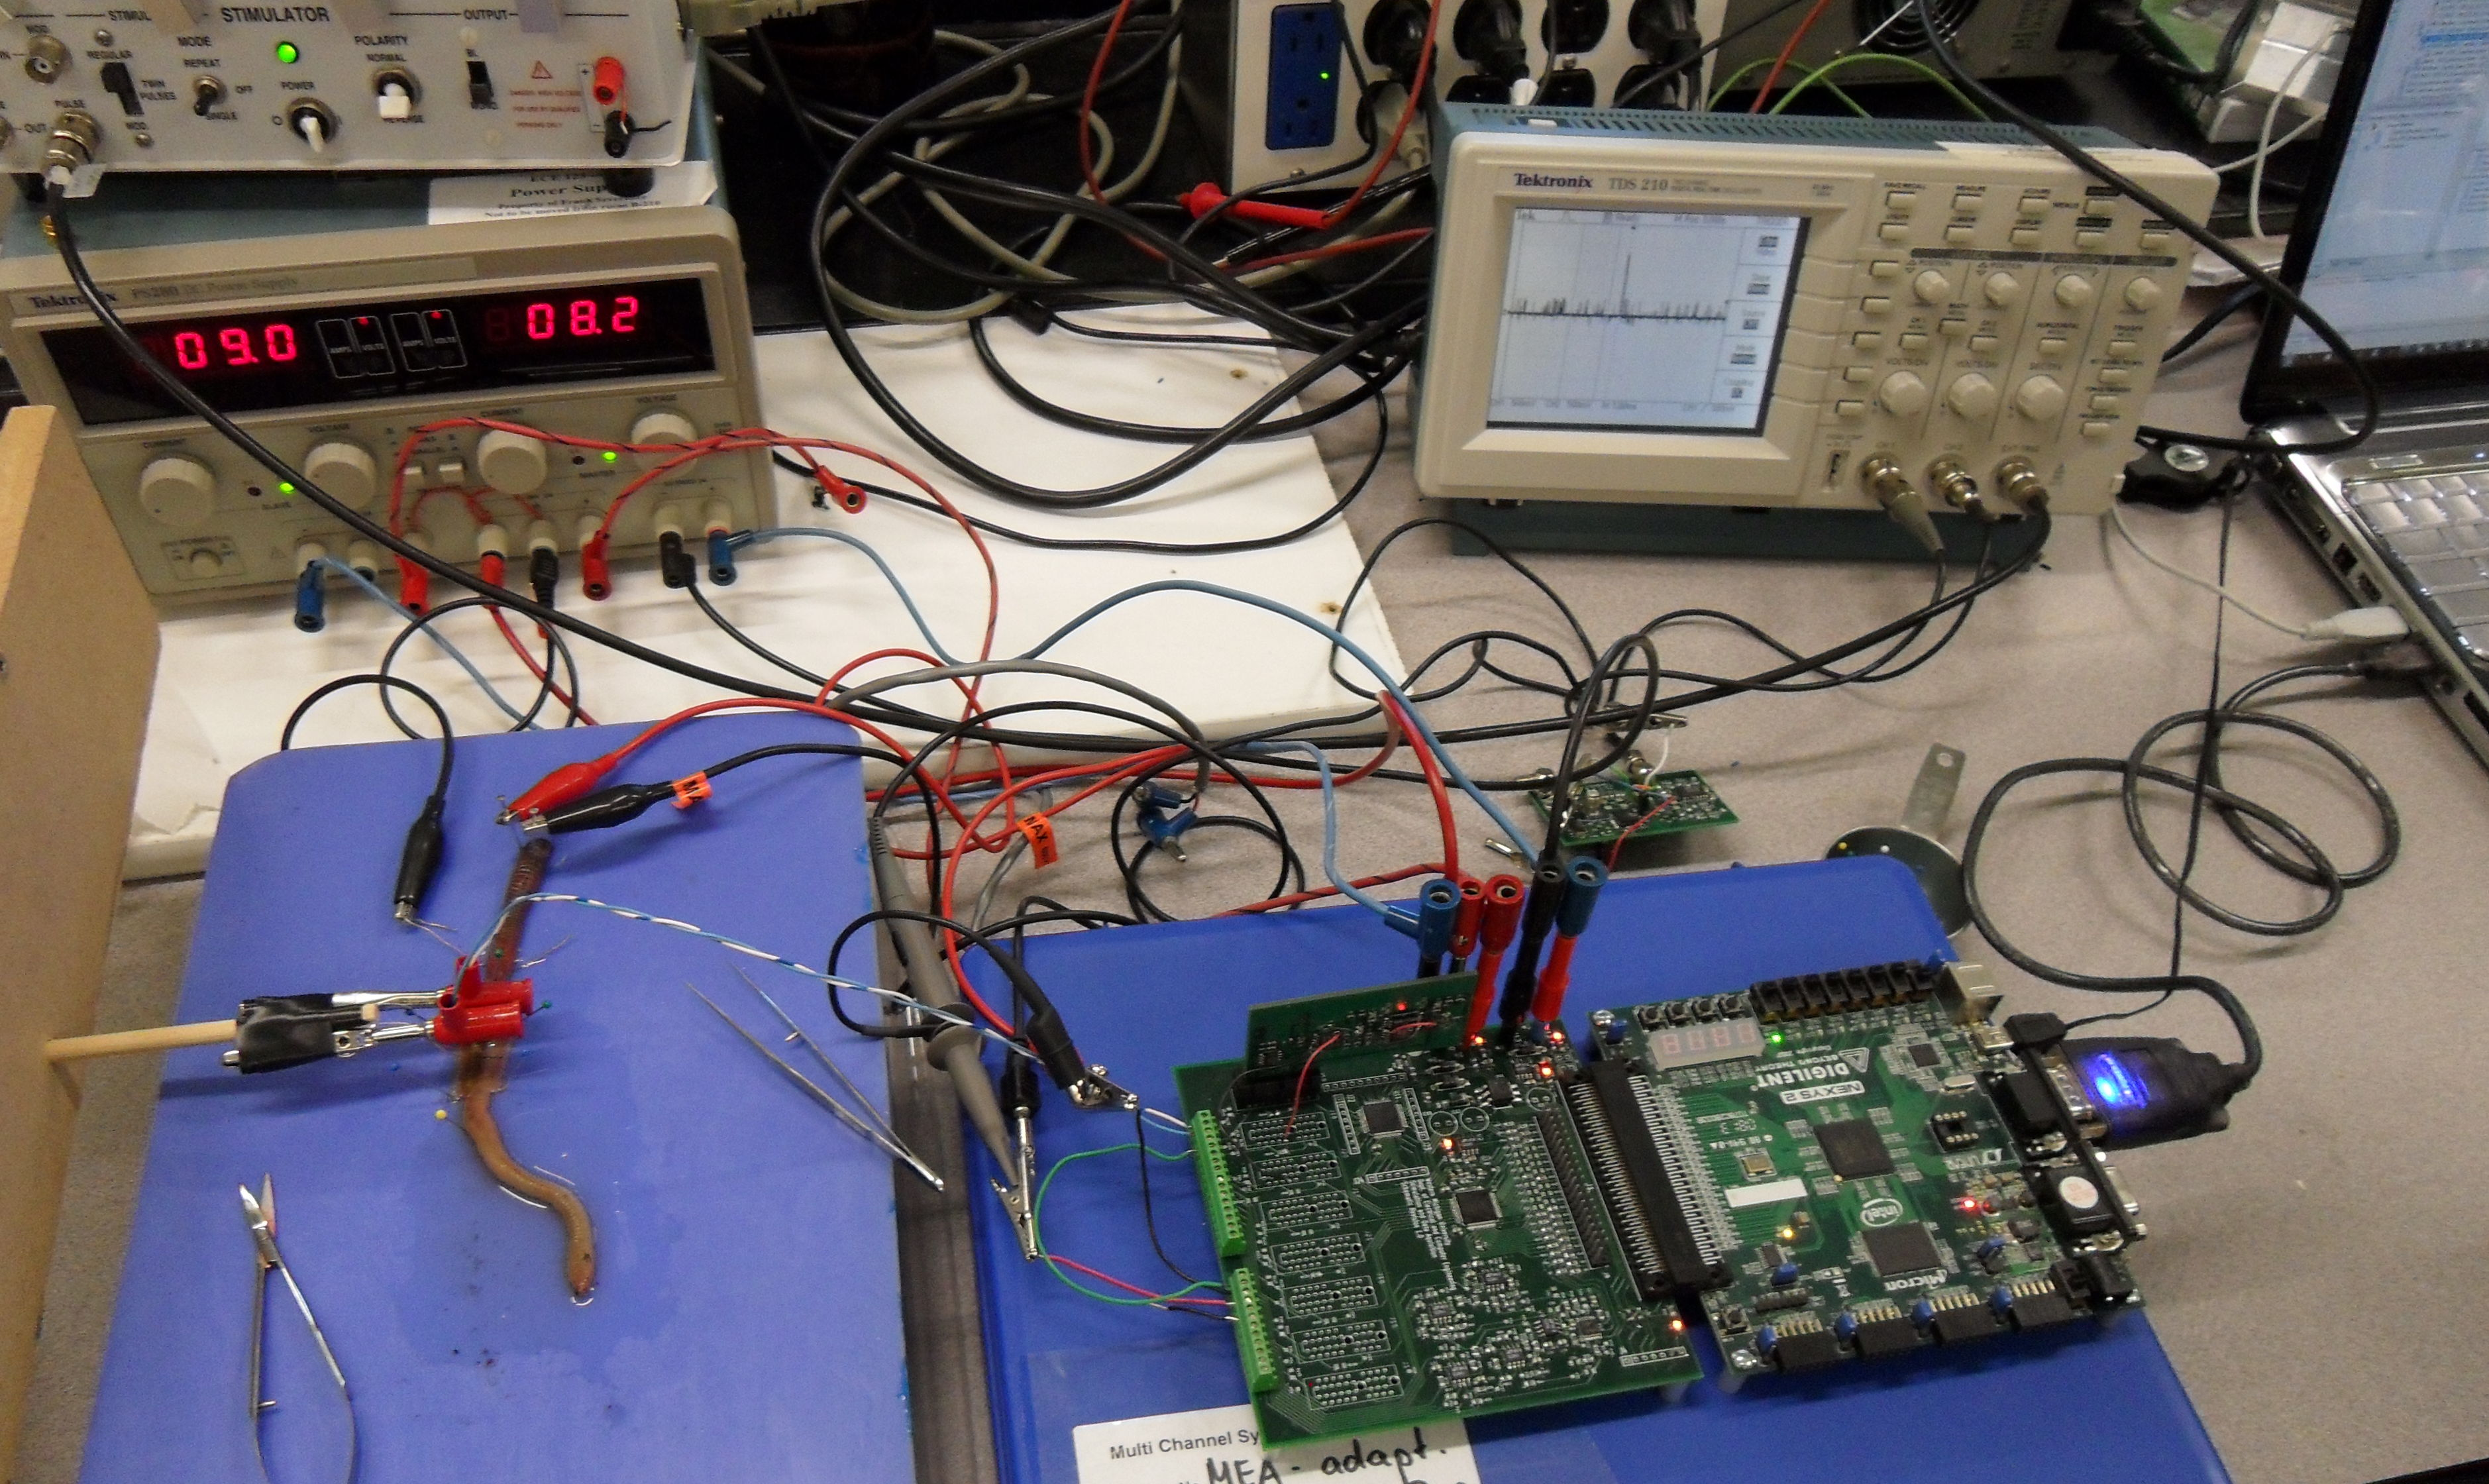
\includegraphics[width=\textwidth-0.75in]{./figures/EWSetupPic} 
	\caption{The Data Acquisition and Stimulation System connected in parallel with a previously validated recording system\label{fig:EWSetupPic}}
	\end{singlespace}
\end{figure}

Data recorded from a $2.0\unit{V}$ stimulation pulse produced a median giant response similar to those seen in~\cite{StahlMSEE} and~\cite{EllingerMSEE}.  Data from the previously validated Preamp and the oscilloscope was plotted on top of the data from the Data Acquisition and Stimulation System using a GNU Octave script.  Data from the oscilloscope and the Data Acquisition and Stimulation System can be seen in Figure~\ref{fig:EWMedResp} and the data appears to be in very close agreement.

\begin{figure}[H]
	\begin{singlespace}
	\centering 
		\resizebox{\textwidth-0.5in}{!}{% GNUPLOT: LaTeX picture with Postscript
\begingroup
  \makeatletter
  \providecommand\color[2][]{%
    \GenericError{(gnuplot) \space\space\space\@spaces}{%
      Package color not loaded in conjunction with
      terminal option `colourtext'%
    }{See the gnuplot documentation for explanation.%
    }{Either use 'blacktext' in gnuplot or load the package
      color.sty in LaTeX.}%
    \renewcommand\color[2][]{}%
  }%
  \providecommand\includegraphics[2][]{%
    \GenericError{(gnuplot) \space\space\space\@spaces}{%
      Package graphicx or graphics not loaded%
    }{See the gnuplot documentation for explanation.%
    }{The gnuplot epslatex terminal needs graphicx.sty or graphics.sty.}%
    \renewcommand\includegraphics[2][]{}%
  }%
  \providecommand\rotatebox[2]{#2}%
  \@ifundefined{ifGPcolor}{%
    \newif\ifGPcolor
    \GPcolorfalse
  }{}%
  \@ifundefined{ifGPblacktext}{%
    \newif\ifGPblacktext
    \GPblacktexttrue
  }{}%
  % define a \g@addto@macro without @ in the name:
  \let\gplgaddtomacro\g@addto@macro
  % define empty templates for all commands taking text:
  \gdef\gplbacktext{}%
  \gdef\gplfronttext{}%
  \makeatother
  \ifGPblacktext
    % no textcolor at all
    \def\colorrgb#1{}%
    \def\colorgray#1{}%
  \else
    % gray or color?
    \ifGPcolor
      \def\colorrgb#1{\color[rgb]{#1}}%
      \def\colorgray#1{\color[gray]{#1}}%
      \expandafter\def\csname LTw\endcsname{\color{white}}%
      \expandafter\def\csname LTb\endcsname{\color{black}}%
      \expandafter\def\csname LTa\endcsname{\color{black}}%
      \expandafter\def\csname LT0\endcsname{\color[rgb]{1,0,0}}%
      \expandafter\def\csname LT1\endcsname{\color[rgb]{0,1,0}}%
      \expandafter\def\csname LT2\endcsname{\color[rgb]{0,0,1}}%
      \expandafter\def\csname LT3\endcsname{\color[rgb]{1,0,1}}%
      \expandafter\def\csname LT4\endcsname{\color[rgb]{0,1,1}}%
      \expandafter\def\csname LT5\endcsname{\color[rgb]{1,1,0}}%
      \expandafter\def\csname LT6\endcsname{\color[rgb]{0,0,0}}%
      \expandafter\def\csname LT7\endcsname{\color[rgb]{1,0.3,0}}%
      \expandafter\def\csname LT8\endcsname{\color[rgb]{0.5,0.5,0.5}}%
    \else
      % gray
      \def\colorrgb#1{\color{black}}%
      \def\colorgray#1{\color[gray]{#1}}%
      \expandafter\def\csname LTw\endcsname{\color{white}}%
      \expandafter\def\csname LTb\endcsname{\color{black}}%
      \expandafter\def\csname LTa\endcsname{\color{black}}%
      \expandafter\def\csname LT0\endcsname{\color{black}}%
      \expandafter\def\csname LT1\endcsname{\color{black}}%
      \expandafter\def\csname LT2\endcsname{\color{black}}%
      \expandafter\def\csname LT3\endcsname{\color{black}}%
      \expandafter\def\csname LT4\endcsname{\color{black}}%
      \expandafter\def\csname LT5\endcsname{\color{black}}%
      \expandafter\def\csname LT6\endcsname{\color{black}}%
      \expandafter\def\csname LT7\endcsname{\color{black}}%
      \expandafter\def\csname LT8\endcsname{\color{black}}%
    \fi
  \fi
  \setlength{\unitlength}{0.0500bp}%
  \begin{picture}(11520.00,8640.00)%
    \gplgaddtomacro\gplbacktext{%
      \colorrgb{0.00,0.00,0.00}%
      \put(860,1380){\makebox(0,0)[r]{\strut{}-0.4}}%
      \colorrgb{0.00,0.00,0.00}%
      \put(860,2860){\makebox(0,0)[r]{\strut{}-0.2}}%
      \colorrgb{0.00,0.00,0.00}%
      \put(860,4339){\makebox(0,0)[r]{\strut{}0}}%
      \colorrgb{0.00,0.00,0.00}%
      \put(860,5819){\makebox(0,0)[r]{\strut{}0.2}}%
      \colorrgb{0.00,0.00,0.00}%
      \put(860,7299){\makebox(0,0)[r]{\strut{}0.4}}%
      \colorrgb{0.00,0.00,0.00}%
      \put(1905,440){\makebox(0,0){\strut{}0}}%
      \colorrgb{0.00,0.00,0.00}%
      \put(3756,440){\makebox(0,0){\strut{}2}}%
      \colorrgb{0.00,0.00,0.00}%
      \put(5607,440){\makebox(0,0){\strut{}4}}%
      \colorrgb{0.00,0.00,0.00}%
      \put(7458,440){\makebox(0,0){\strut{}6}}%
      \colorrgb{0.00,0.00,0.00}%
      \put(9308,440){\makebox(0,0){\strut{}8}}%
      \colorrgb{0.00,0.00,0.00}%
      \put(11159,440){\makebox(0,0){\strut{}10}}%
      \colorrgb{0.00,0.00,0.00}%
      \put(160,4339){\rotatebox{90}{\makebox(0,0){\strut{}Voltage ($V$)}}}%
      \colorrgb{0.00,0.00,0.00}%
      \put(6069,140){\makebox(0,0){\strut{}Time ($ms$)}}%
      \csname LTb\endcsname%
      \put(6069,8339){\makebox(0,0){\strut{}Response to $2V$ Stimulation}}%
    }%
    \gplgaddtomacro\gplfronttext{%
      \csname LTb\endcsname%
      \put(10256,7876){\makebox(0,0)[r]{\strut{}Oscilloscope Data}}%
      \csname LTb\endcsname%
      \put(10256,7676){\makebox(0,0)[r]{\strut{}ADC Data}}%
      \colorrgb{0.00,0.00,0.00}%
      \put(3987,3230){\makebox(0,0)[l]{\strut{}Stimulus Artifact}}%
      \put(4913,6189){\makebox(0,0)[l]{\strut{}Median Giant Response}}%
    }%
    \gplbacktext
    \put(0,0){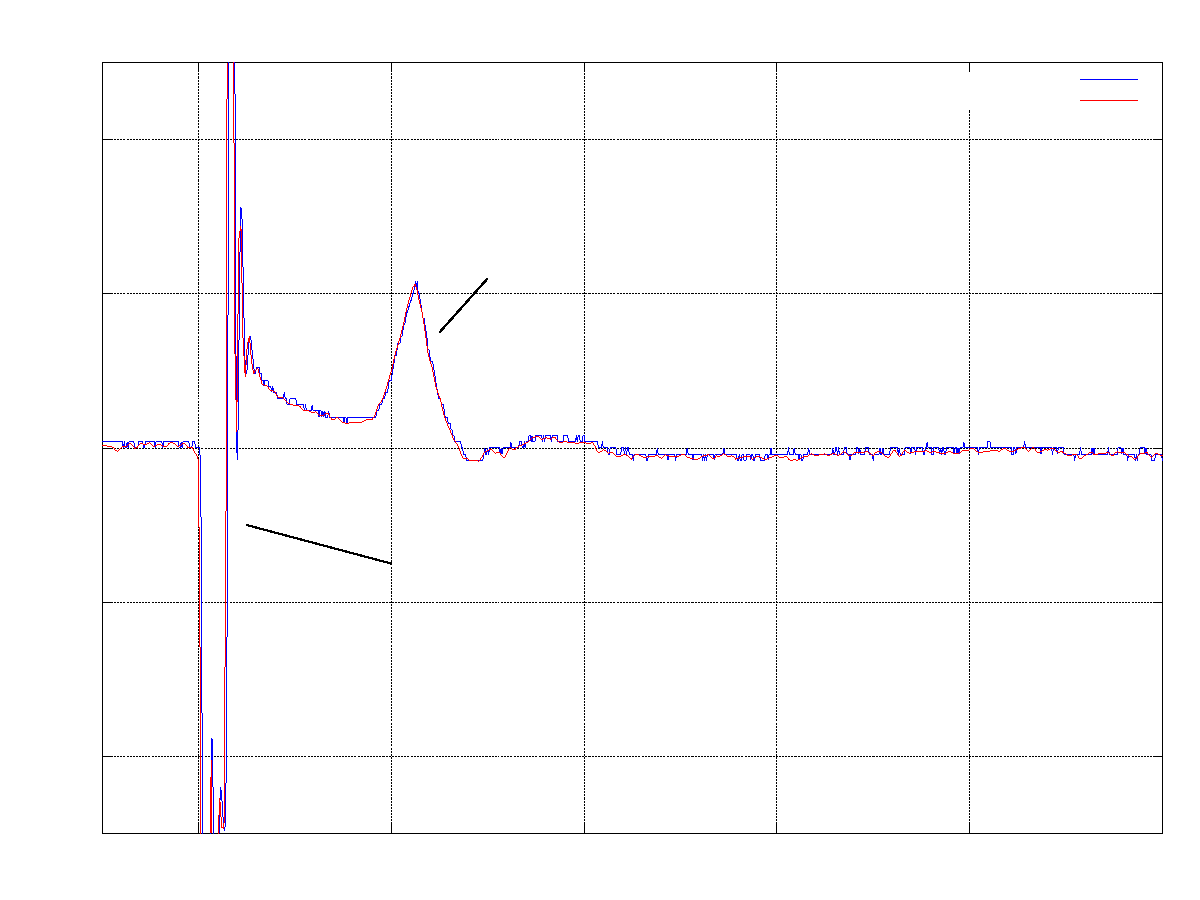
\includegraphics{median}}%
    \gplfronttext
  \end{picture}%
\endgroup
}
	\caption{Earthworm response to $2.0\unit{V}$ stimulation pulse generated by the Data Acquisition and Stimulation System with data recorded by the oscilloscope and by the ADC on the Data Acquisition and Stimulation System\label{fig:EWMedResp}}
	\end{singlespace}
\end{figure}

Data recorded from a $3.5\unit{V}$ stimulation pulse produced median and lateral giant responses similar to those seen in~\cite{StahlMSEE} and~\cite{EllingerMSEE}.  The data shown in Figure~\ref{fig:EWLatResp} exhibits close agreement between the Data Acquisition and Stimulation System and the previously validated Preamp.

\begin{figure}[H]
	\begin{singlespace}
	\centering 
		\resizebox{\textwidth-0.5in}{!}{% GNUPLOT: LaTeX picture with Postscript
\begingroup
  \makeatletter
  \providecommand\color[2][]{%
    \GenericError{(gnuplot) \space\space\space\@spaces}{%
      Package color not loaded in conjunction with
      terminal option `colourtext'%
    }{See the gnuplot documentation for explanation.%
    }{Either use 'blacktext' in gnuplot or load the package
      color.sty in LaTeX.}%
    \renewcommand\color[2][]{}%
  }%
  \providecommand\includegraphics[2][]{%
    \GenericError{(gnuplot) \space\space\space\@spaces}{%
      Package graphicx or graphics not loaded%
    }{See the gnuplot documentation for explanation.%
    }{The gnuplot epslatex terminal needs graphicx.sty or graphics.sty.}%
    \renewcommand\includegraphics[2][]{}%
  }%
  \providecommand\rotatebox[2]{#2}%
  \@ifundefined{ifGPcolor}{%
    \newif\ifGPcolor
    \GPcolorfalse
  }{}%
  \@ifundefined{ifGPblacktext}{%
    \newif\ifGPblacktext
    \GPblacktexttrue
  }{}%
  % define a \g@addto@macro without @ in the name:
  \let\gplgaddtomacro\g@addto@macro
  % define empty templates for all commands taking text:
  \gdef\gplbacktext{}%
  \gdef\gplfronttext{}%
  \makeatother
  \ifGPblacktext
    % no textcolor at all
    \def\colorrgb#1{}%
    \def\colorgray#1{}%
  \else
    % gray or color?
    \ifGPcolor
      \def\colorrgb#1{\color[rgb]{#1}}%
      \def\colorgray#1{\color[gray]{#1}}%
      \expandafter\def\csname LTw\endcsname{\color{white}}%
      \expandafter\def\csname LTb\endcsname{\color{black}}%
      \expandafter\def\csname LTa\endcsname{\color{black}}%
      \expandafter\def\csname LT0\endcsname{\color[rgb]{1,0,0}}%
      \expandafter\def\csname LT1\endcsname{\color[rgb]{0,1,0}}%
      \expandafter\def\csname LT2\endcsname{\color[rgb]{0,0,1}}%
      \expandafter\def\csname LT3\endcsname{\color[rgb]{1,0,1}}%
      \expandafter\def\csname LT4\endcsname{\color[rgb]{0,1,1}}%
      \expandafter\def\csname LT5\endcsname{\color[rgb]{1,1,0}}%
      \expandafter\def\csname LT6\endcsname{\color[rgb]{0,0,0}}%
      \expandafter\def\csname LT7\endcsname{\color[rgb]{1,0.3,0}}%
      \expandafter\def\csname LT8\endcsname{\color[rgb]{0.5,0.5,0.5}}%
    \else
      % gray
      \def\colorrgb#1{\color{black}}%
      \def\colorgray#1{\color[gray]{#1}}%
      \expandafter\def\csname LTw\endcsname{\color{white}}%
      \expandafter\def\csname LTb\endcsname{\color{black}}%
      \expandafter\def\csname LTa\endcsname{\color{black}}%
      \expandafter\def\csname LT0\endcsname{\color{black}}%
      \expandafter\def\csname LT1\endcsname{\color{black}}%
      \expandafter\def\csname LT2\endcsname{\color{black}}%
      \expandafter\def\csname LT3\endcsname{\color{black}}%
      \expandafter\def\csname LT4\endcsname{\color{black}}%
      \expandafter\def\csname LT5\endcsname{\color{black}}%
      \expandafter\def\csname LT6\endcsname{\color{black}}%
      \expandafter\def\csname LT7\endcsname{\color{black}}%
      \expandafter\def\csname LT8\endcsname{\color{black}}%
    \fi
  \fi
  \setlength{\unitlength}{0.0500bp}%
  \begin{picture}(11520.00,8640.00)%
    \gplgaddtomacro\gplbacktext{%
      \colorrgb{0.00,0.00,0.00}%
      \put(860,640){\makebox(0,0)[r]{\strut{}-1.5}}%
      \colorrgb{0.00,0.00,0.00}%
      \put(860,1873){\makebox(0,0)[r]{\strut{}-1}}%
      \colorrgb{0.00,0.00,0.00}%
      \put(860,3106){\makebox(0,0)[r]{\strut{}-0.5}}%
      \colorrgb{0.00,0.00,0.00}%
      \put(860,4340){\makebox(0,0)[r]{\strut{}0}}%
      \colorrgb{0.00,0.00,0.00}%
      \put(860,5573){\makebox(0,0)[r]{\strut{}0.5}}%
      \colorrgb{0.00,0.00,0.00}%
      \put(860,6806){\makebox(0,0)[r]{\strut{}1}}%
      \colorrgb{0.00,0.00,0.00}%
      \put(860,8039){\makebox(0,0)[r]{\strut{}1.5}}%
      \colorrgb{0.00,0.00,0.00}%
      \put(1905,440){\makebox(0,0){\strut{}0}}%
      \colorrgb{0.00,0.00,0.00}%
      \put(3756,440){\makebox(0,0){\strut{}2}}%
      \colorrgb{0.00,0.00,0.00}%
      \put(5607,440){\makebox(0,0){\strut{}4}}%
      \colorrgb{0.00,0.00,0.00}%
      \put(7458,440){\makebox(0,0){\strut{}6}}%
      \colorrgb{0.00,0.00,0.00}%
      \put(9308,440){\makebox(0,0){\strut{}8}}%
      \colorrgb{0.00,0.00,0.00}%
      \put(11159,440){\makebox(0,0){\strut{}10}}%
      \colorrgb{0.00,0.00,0.00}%
      \put(160,4339){\rotatebox{90}{\makebox(0,0){\strut{}Voltage ($V$)}}}%
      \colorrgb{0.00,0.00,0.00}%
      \put(6069,140){\makebox(0,0){\strut{}Time ($ms$)}}%
      \csname LTb\endcsname%
      \put(6069,8339){\makebox(0,0){\strut{}Response to $3.5V$ Stimulation}}%
    }%
    \gplgaddtomacro\gplfronttext{%
      \csname LTb\endcsname%
      \put(10256,7876){\makebox(0,0)[r]{\strut{}Oscilloscope Data}}%
      \csname LTb\endcsname%
      \put(10256,7676){\makebox(0,0)[r]{\strut{}ADC Data}}%
      \colorrgb{0.00,0.00,0.00}%
      \put(3987,2736){\makebox(0,0)[l]{\strut{}Stimulus Artifact}}%
      \put(4913,5943){\makebox(0,0)[l]{\strut{}Median Giant Response}}%
      \put(8614,5943){\makebox(0,0)[l]{\strut{}Lateral Giant Response}}%
    }%
    \gplbacktext
    \put(0,0){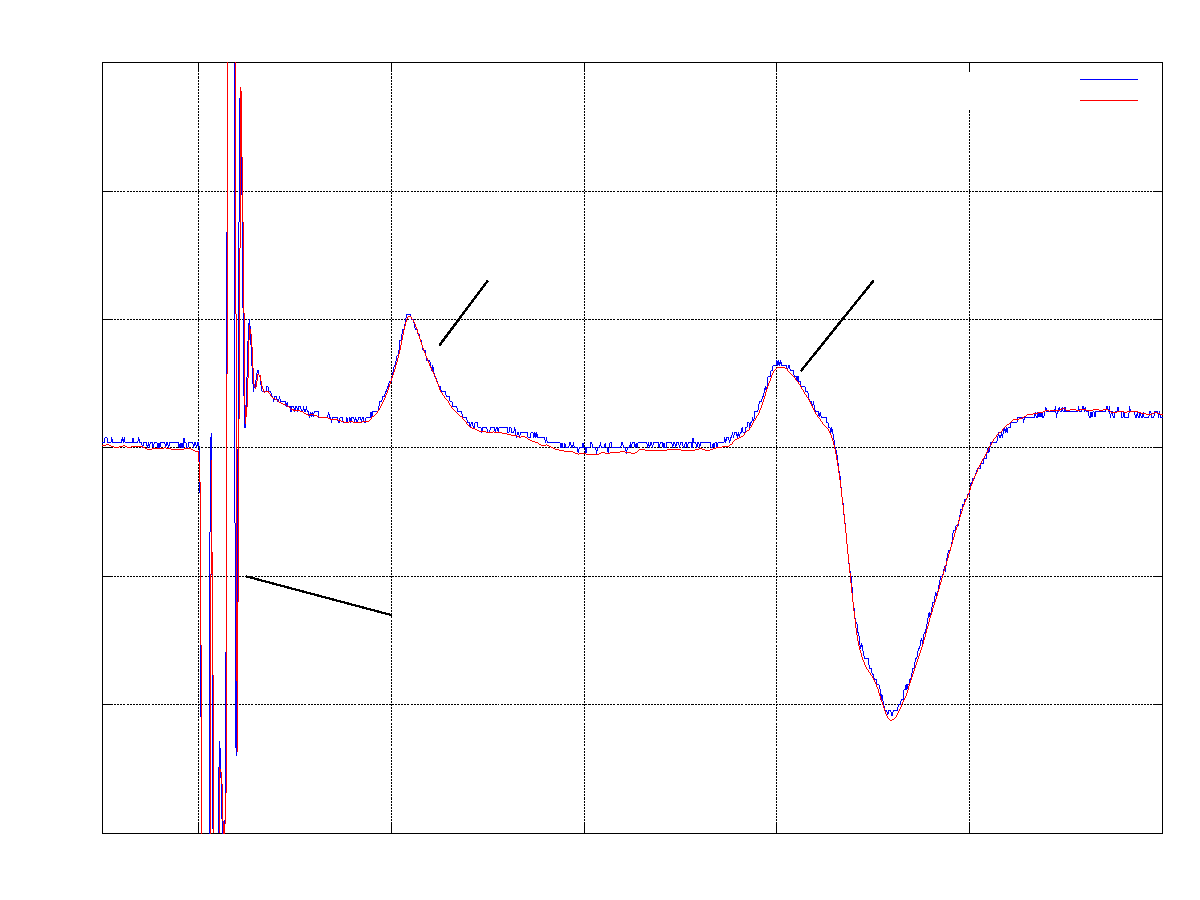
\includegraphics{lateral}}%
    \gplfronttext
  \end{picture}%
\endgroup
}
	\caption{Earthworm response to $3.5\unit{V}$ stimulation pulse generated by the Data Acquisition and Stimulation System with data recorded by the oscilloscope and by the ADC on the Data Acquisition and Stimulation System\label{fig:EWLatResp}}
	\end{singlespace}
\end{figure}


\section[Specifications Review]{Specifications Review\footnote{This section is co-authored with Kyle Batzer,~\cite{BatzerMSEE}}}

%Review how well the requirements were met
This section reviews the specifications set forth in section~\ref{sec:spec} and shows how well the Data Acquisition and Stimulation System described in this thesis meets those specifications.

\begin{enumerate}

\item Provide a platform for performing electrophysiology experiments with earthworms as described in~\cite{Olivo,KuehJellies}

Successful accomplishment of the earthworm experiment is shown in section~\ref{sec:results}.

	\begin{enumerate}
	
	\item Produce a voltage-controlled stimulation pulse that is a square wave with widths from 0.01ms to 100ms and amplitudes from 0.1V to 10V
	
	The FPGA and Data Acquisition and Stimulation System Control Center (DASCC) are capable of defining a stimulation waveform that updates the DAC output with a period as short as $1\unit{\mu s}$ and storing up to 4096 waveform samples with variable sample periods from $1\unit{\mu s}$ to 65.536ms~\cite{BatzerMSEE}.  The DAC has a slew rates of $1.5\unit{V}/\unit{\mu s}$~\cite{AD5678ds} and a differential output voltage range of $\pm 14.8\unit{V}$ as shown in section~\ref{sec:DOA}.
	
	\item Produce single stimulation pulses or multiple pulses at rates from 1Hz to 10Hz
	
	The FPGA and DASCC are capable of defining a stimulation waveform over 1s in length and repeating the waveform indefinitely~\cite{BatzerMSEE}.
	
	\item Provide at least one differential recording channel
	
	There is the potential for up to eight recording channels, each with a Preamp that has a differential input as shown in section~\ref{sec:preamp}.
	
	\item Record action potential voltage from the time of the stimulation pulse for a minimum duration of 20ms
	
	Data collected for results in section~\ref{sec:results} is more than 1s in duration.
	
	\item Plot the recorded voltage
	
	The DASCC is capable of plotting recorded data~\cite{BatzerMSEE}.
	
	\item Store the recorded voltage to a non-proprietary, standard file format
	
	The DASCC is capable of exporting recorded data to a comma separated values (CSV) text file~\cite{BatzerMSEE}.
	
	\end{enumerate}
	

\item Provide a platform for stimulation and recording of neuron cell cultures in a portion of an MEA

Interfacing the DASS with the MEA is not yet tested

	\begin{enumerate}
	
	\item Provide at least four recording channels
	
	Eight recording electrodes can be connected to the DASS and stored as digital samples as described in sections~\ref{sec:adc} and~\ref{sec:preamp}.
	
	\item Store data from recording channels continuously
	
	The data recording time limit has not been fully tested.
	
	\item Provide at least four voltage-controlled arbitrary stimulation channels
	
	The DASCC is capable of loading an arbitrary waveform as defined by a text file into the DASS, which outputs the waveform using the AD5678 with four DAC outputs shown in section~\ref{sec:dac}~\cite{BatzerMSEE}
	
	\item Output single-ended stimulation signals on recording electrodes and add culture voltage offset to the signal
	
	The stimulation signals are routed to the Preamp boards which output the stimulation signals on the recording electrodes and add the culture voltage offset as described in section~\ref{sec:preamp}
	
	\item Provide an interface that can specify stimulation waveforms, locations, and intervals that can be updated based on data from the recording electrodes
	
	The DASCC provides a scripting language for defining recording intervals, stimulation waveforms, and stimulation intervals but does not have provisions for analyzing recorded data and adjusting stimulation strategy~\cite{BatzerMSEE}
	
	\end{enumerate}

\item Utilize Low-Noise Amplifier described in~\cite{StahlMSEE}

The Low-Noise Amplifier, also know as the Preamp, is successfully utilized with the DASS; though, not all features are tested.

	\begin{enumerate}
	
	\item Connect to each Low-Noise Amplifier channel with a PCI-Express card edge connector
	
	Eight PCI-Express card edge connector sockets are available on the Electrophysiology Interface board as described in section~\ref{sec:preamp}
	
	\item Provide $\pm 7\unit{V}$ to $\pm 15\unit{V}$ analog voltage supplies and ground via the card edge connector
	
	The Electrophysiology Interface board connects its analog voltage supply inputs, which tolerate $\pm 7\unit{V}$ to $\pm 15\unit{V}$, to the Preamp connectors as described sections~\ref{sec:power} and~\ref{sec:preamp}.
	
	\item Provide ability to independently switch four digital inputs for each channel, $0_{\mathrm{IH}}=0.8\unit{V}$ and $1_{\mathrm{IL}}=2.4\unit{V}$
	
	The CPLD on the Electrophysiology Interface board enables the FPGA to control each digital input on every Preamp channel and voltage compatibility is shown in section~\ref{sec:cpld}, but a logic configuration for the CPLD is not written.
	
	\item Route differential analog input to the card edge connector for each channel
	
	The differential inputs of the Preamps are routed to a terminal block for simple connection to recording electrodes as described in section~\ref{sec:preamp}.
	
	\item Convert the 20Hz to 14.6kHz analog output signal~\cite{StahlMSEE} to digital samples %with a resolution better than (XX)$V/LSB$ [check with references or base number on oscilloscope resolution]
	
	An AD7606 ADC converts the Preamp output voltage to digital samples, has an analog low-pass input filter with a corner frequency of 23kHz, and can sample at up to $200\unit{kS}/\unit{s}$, satisfying the sampling theorem, as described in section~\ref{sec:adc}
	
	\item Route a single-ended stimulation signal to each channel
	
	Four unique stimulation channels with differential outputs are connected single-endedly to the eight Preamp connectors as described in section~\ref{sec:preamp}.
	
	\end{enumerate}
	
\item Additional requirements

	\begin{enumerate}
	
%	\item Produce arbitrary stimulation waveforms with minimum bandwidth (XX)$Hz$ and minimum slew rate (XX)$V / \mu s$
	
	\item Employ good circuit design and layout practices
	
	Good design and layout practice is attempted throughout the design of the Electrophysiology Interface board and in connecting all the components of the DASS.  For example, bulk and decoupling capacitors are utilized, four-layer PCB construction is used, and analog and digital power supply isolation is attempted.  Although, there may be better strategies for analog and digital isolation than was used in the design of the Electrophysiology Interface board and some of those strategies are discussed in section~\ref{sec:ground}.
	
%	[Anything else that doesn't fit in the above categories]
	
	\end{enumerate}
	
\end{enumerate}


\section{Scaling the DASS Hardware to 60 Channels}\label{sec:scaling}

%An overview of the elements of the Nexys2 and Stimulation and Data Acquisition Board that could be copied to build the hardware for a 60 channel MEA stimulation and data acquisition system.
Experiments with cultured neurons on an MEA requires the ability to stimulate and record on all 60 electrodes of the MEA.  The developed Data Acquisition and Stimulation System (DASS) only has the capability of recording data on eight electrodes and outputing four unique stimulation waveforms on those electrodes.  A 60-channel system could be developed by testing and refining, as needed, the hardware and software design principles used by the DASS on a portion of a MEA.  Figure~\ref{fig:System64} shows one possible incarnation of the hardware for a system capable of stimulating and recording with up to 64 electrodes, which is four more channels than necessary for a 60 electrode MEA.

\begin{figure}[htb]
	\begin{singlespace}
	\centering	
		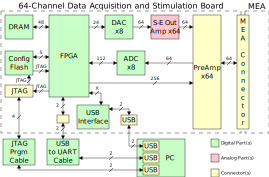
\includegraphics{./figures/System64} 
	\caption{Block diagram of a proposed 64-channel system based on the RTSC board and Electrophysiology Interface board design\label{fig:System64}}
	\end{singlespace}
\end{figure}

The proposed system expands on the circuit designs of the DASS.  A custom PCB connects to the MEA and has a PCI-Express card edge connector socket to interface a PreAmp board to each electrode on the MEA.  The PreAmp voltage output is recorded by eight AD7606 eight-channel ADC components.  Eight AD5678 components contain four 16-bit DACs and four 12-bit DACs each for a total of 64 DAC outputs, and analog amplification circuitry conditions the DAC outputs, providing 64 single-ended stimulation signals to the Preamp boards.  An FPGA on a custom board offers many more IO pins than are available on most development kits; thus, there are likely to be enough IO pins to control the four digital inputs of each PreAmp board without the need for a CPLD for IO expansion.

The FPGA controls the eight AD7606 ADCs and eight AD5678 DACs.  External RAM memory is likely needed to store stimulation waveform data.  A configuration flash memory chip loads the FPGA configuration upon power-up.  A JTAG programming cable eliminates the need for custom microcontroller firmware to load FPGA configurations into the FPGA or configuration flash memory.  A USB to UART cable allows commands to be communicated to the FPGA from the PC with minimal circuitry on the PCB.  And, a microcontroller with a USB PHY allows for fast data transfer of electrode recordings to the PC.

Information that could be acquired by testing this design with the DASS include: confirming whether 12 bits of DAC resolution is sufficient for MEA experiments, determining optimal timing of PreAmp digital control signals, determining which control signals for the ADC and DAC need to be controlled by the FPGA and which can be permanently tied to a logic level, testing data throughput for the USB interface, and, if data transfer speed is found to be insufficient, testing alternative USB2 or USB3 capable microcontrollers.  One area that will need to be tested outside of the current embodiment of the DASS is PCB assembly with ball grid array (BGA) packages: the number of IO pins and logic gates required by a 64-channel system will necessitate the use of a BGA packaged FPGA.


\section{Conclusions}

The work of many students in the Neurobiology Engineering Laboratory at Western Michigan University made the completion of the Data Acquisition and Stimulation System (DASS) possible.  Utilizing the documentation and knowledge gained from previous groups~\cite{ArmstrongSD,McCaskeyPackaralJohnVandeusen07,CarusoDaiekJones,StahlMSEE,BatzerCorsiCrampton} and the concurrent efforts of fellow graduate student, Mr.~Kyle Batzer~\cite{BatzerMSEE}, a custom multi-channel data acquisition and stimulation system has been developed for use in electrophysiology experiments at the Neurobiology Engineering Laboratory.  Validation of the system by performing a standard electrophysiology experiment was, again, aided by the experience of students' previous design projects~\cite{StahlMSEE,EllingerMSEE}.

Designing hardware for a mixed digital and analog system can be a challenge.  Being able to refer to previous work reduces design time and risk.  Thorough documentation in this thesis also reduces risk and aides in the subsequent use of the system.  A PCB can be an expensive investment (see appendix~\ref{sec:bom}), and the utilization of headers and $0\unit{\Omega}$ resistors in the design of the Electrophysiology Interface board allows the few layout mistakes to be rectified, as shown in appendix~\ref{sec:errata}.

Application of the DASS by future students in electrophysiology experiments will require knowledge of electrical engineering.  The hardware, even though it does contain some protection circuitry, can be damaged by misapplication of power or incorrect connection of inputs and outputs.  The documentation in this thesis will make understanding the DASS attainable for an electrical engineering student who devotes a month or two to part-time study of the system.  The documentation can also be used for a future project that would implement a system, described in section~\ref{sec:scaling}, with enough channels to fully exploit an Microelectrode Array (MEA) with 60 electrodes.  Such a project may be too ambitious for a senior design group or graduate student to complete alone in one year, but a senior design group or graduate student that has experience working with the DASS on electrophysiology experiments before beginning such a project could realize a working 60 channel data acquisition and stimulation system.

Personally, I broadened my knowledge of electronic circuit design in creating the Electrophysiology Interface board for the DASS, gained experience collaborating with a talented firmware and software designer, explored another field by learning enough neurophysiology to perform and design hardware for electrophysiology experiments, and gained confidence in my circuit and PCB design skills by having a PCB manufactured that was used successfully in an electrophysiology experiment.



\newpage
\appendix
\appendixpage
\addappheadtotoc

\section{Electrophysiology Interface Board Schematic}\label{sec:schematic}

The following is the hierarchical schematic for the Electrophysiology Interface Board.  The schematic was created using the KiCAD open source EDA software suite.

The first page of the schematic contains most of the connectors on the Electrophysiology Interface Board.  Hierarchical blocks in the first schematic page represent following schematic pages with labels on the blocks corresponding to net names in the schematic page represented by the block.  All signals have a scope only within a single schematic page save for the power supply nets, which have a global scope.  The power supply input connectors are shown on page~\pageref{SchematicRev1r0.14}, and since the power nets are global, the hierarchical block on page~\pageref{SchematicRev1r0.1} representing power input connector page, page~\pageref{SchematicRev1r0.14}, is empty of labels.

\newcounter{includepdfpage} % used to allow \pageref to the individual pdf pages http://tex.stackexchange.com/questions/25105/unable-to-link-to-inserted-pages-with-pdfpages
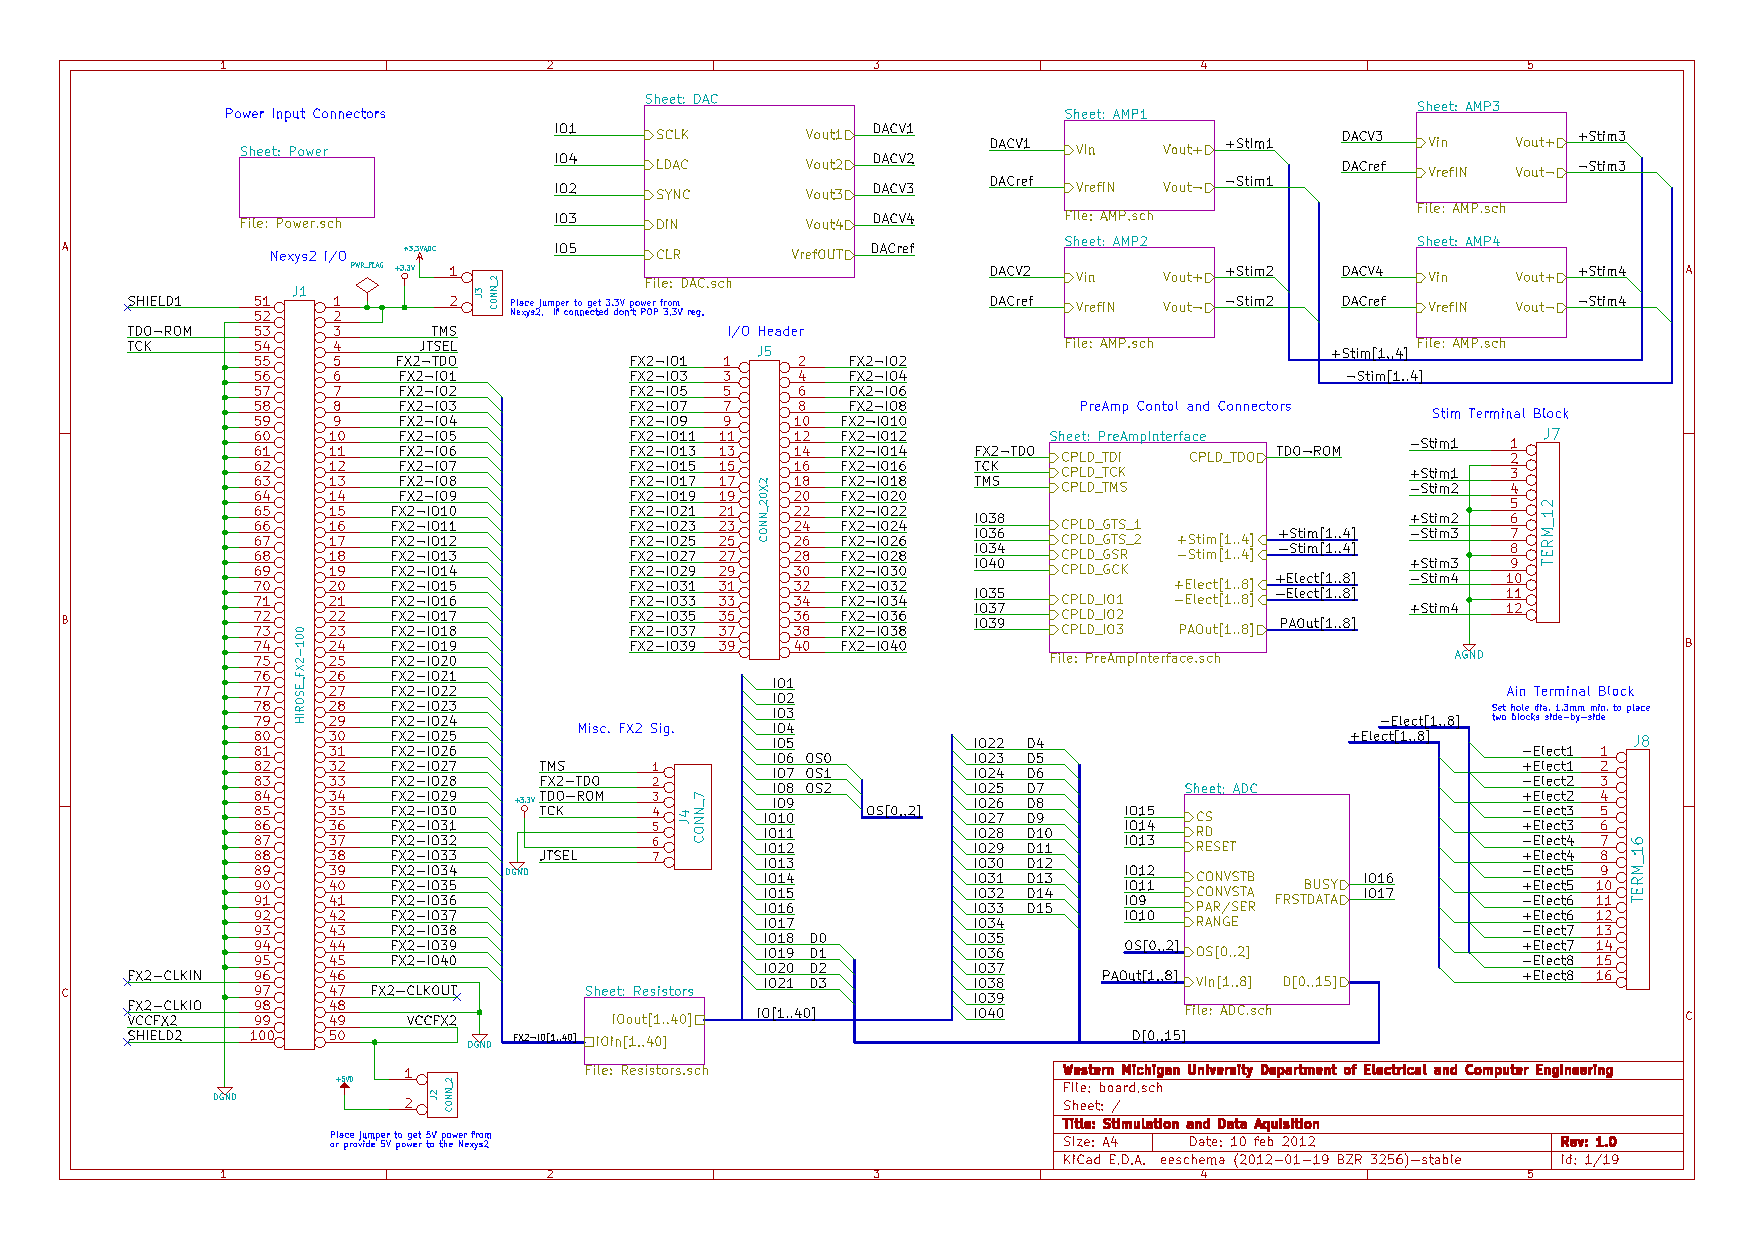
\includepdf[pages=-,link,linkname=SchematicRev1r0,landscape=true,noautoscale,trim=0.38in 0.38in 0.38in 0.38in,clip,width=\textheight,pagecommand={\refstepcounter{includepdfpage}\label{SchematicRev1r0.\theincludepdfpage}}]{./figures/SchematicRev1r0.pdf}

\section{KiCad Gerber File Export Instructions}\label{sec:gerberexp}

Things to note: KiCAD produces gerber files in 274X format, so an aperture list file isn't needed.  Use 8 characters for the file names.  The drill map needs to be precision 2:4 with trailing zeros suppressed.

To generate the gerber and drill files, in Pcbnew, go to file-->plot, see Figure~\ref{fig:plotdialog1}.  Notice that the copper layers, silkscreen, soldermask, and PCB\_Edges layers are selected; that "Exclude PCB Edge layer from other layers" is selected; and that "Use auxiliary axis as origin" is selected.  A folder in the project directory called "gerber" keeps the plotted files organized.  Press "Plot" to generate the files.

\begin{figure}[H]
	\centering 
		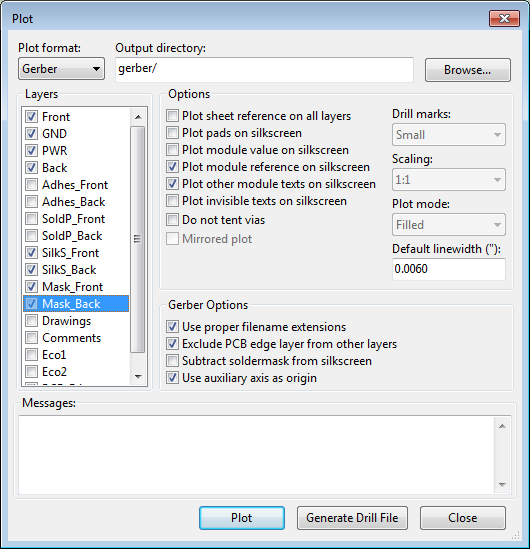
\includegraphics{./figures/plotdialog1} 
	\caption{Pcbnew plot dialog\label{fig:plotdialog1}}
\end{figure}

Advanced Circuits prefers the edge outline of the PCB to be on the silkscreen layer rather than in a separate file.  As set up in Figure~\ref{fig:plotdialog1}, the edges are only in the separate file.  To get the edges on the front silkscreen, see  Figure~\ref{fig:plotdialog2}.  Notice that only the front silkscreen layer is selected and this time "Exclude PCB Edge layer from other layers" is not selected. Press "Plot" to generate the new front silkscreen with the PCB edges.

\begin{figure}[H]
	\centering 
		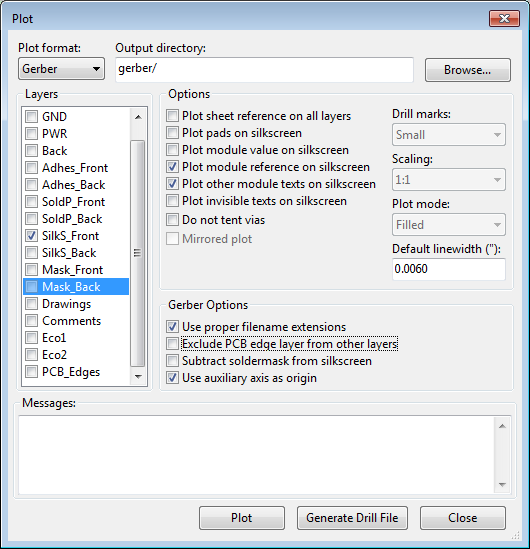
\includegraphics{./figures/plotdialog2} 
	\caption{Pcbnew plot dialog\label{fig:plotdialog2}}
\end{figure}

To generate the drill file, while in file-->plot, press the "Generate Drill File" button.  See  Figure~\ref{fig:drilldialog}.  Notice the Inches, Suppress trailing zeros, 2:4 precision, Drill Map (gerber), and the auxiliary axis that should have been added to the layout are selected (the auxiliary axis was also selected in Figure~\ref{fig:plotdialog1}).  It is necessary to have set the auxiliary axis to a corner of the PCB outline in the main drawing window.  The Drill Map (gerber) selection will produce the additional "fabrication print showing printed circuit board outline with drill pattern and sizes in gerber format."

\begin{figure}[H]
	\centering 
		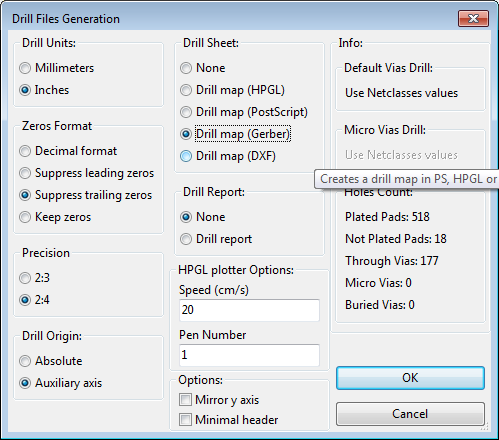
\includegraphics{./figures/drilldialog} 
	\caption{Pcbnew drill dialog\label{fig:drilldialog}}
\end{figure}

When going through the FreeDFM:

You will have to select what each file is.  The program recognizes most files, except for the PCB\_Edges which you want to set as "Drawing/Other" in the drop down box and the GND and PWR layers are "Inner Copper" in the dropdown and another drop down will show up in which you tell it that the files are "Positive" (the filled in areas should have copper as opposed to negative in which the filled in areas are not copper) and GND is layer "2" (or "3") while PWR is layer "3" (or "2") (if th  The .drl file is the Excellion dril file while the .pho file is the fabrication print with drill pattern and sizes in gerber format that should be "Drawing/Other."  %See Figure~\ref{fig:freedfm}

%\begin{landscape}
%\begin{figure}[h]
%	\centering 
%	\begin{singlespace}
%	\begin{subfigure}[b]{0.45\textwidth}
%		\centering 
%		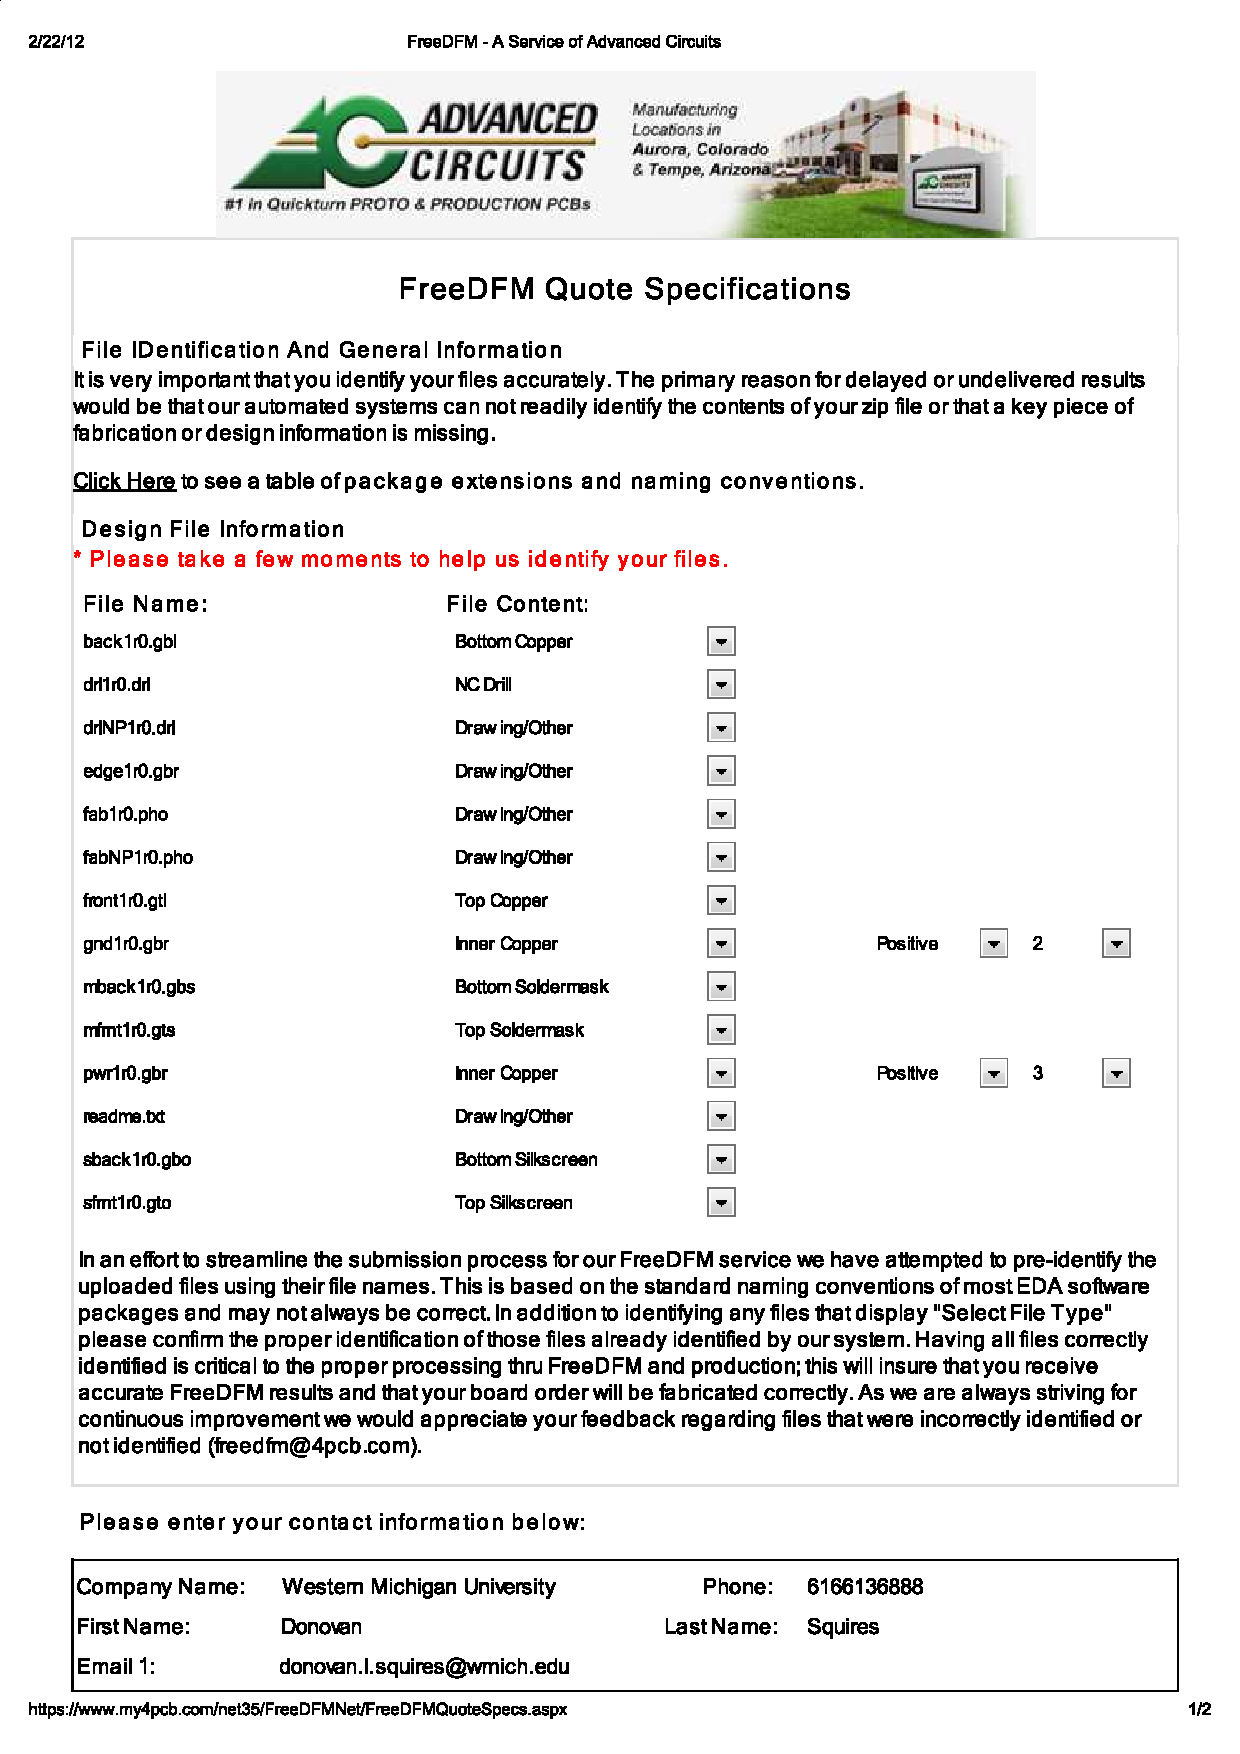
\includegraphics[page=1,height=0.9\textheight]{./figures/FreeDFMupload_120222}
%	\caption{Power plane\label{fig:freedfma}}
%	\end{subfigure}
%	~
%	\begin{subfigure}[b]{0.45\textwidth}
%		\centering 
%		\includegraphics[page=2,height=0.9\textheight]{./figures/FreeDFMupload_120222}
%	\caption{Ground plane\label{fig:freedfmb}}
%	\end{subfigure}
%	\caption{Close clearances on power and ground planes\label{fig:freedfm}}
%	\end{singlespace}
%\end{figure}
%\end{landscape}

When you are ready to place your order:

\begin{enumerate}
	\item Add a README.txt with this information:
	\begin{enumerate}
		\item List of every file name with a brief description as to what it is.
		\item List all non-gerber specs for this job.
		\item Your contact information (include evening phone if you like).
	\end{enumerate}
	\item Change all of the file names to 8 characters + the 3 character extension
	\item Remember that if you place orders later, you will want to have a different zip file name.
\end{enumerate}

\section{Bill of Materials}\label{sec:bom}

Table~\ref{tab:bom} in this section shows the list of components used to populate the Electrophysiology Interface board.  Information from the KiCAD EDA suite, such as reference designator, footprint name (Package), and component value (Designation), is aligned with data from the part supplier, DigiKey\textsuperscript{\textregistered}, such as part number and unit price at the time of purchase.

\begin{landscape}
\renewcommand{\arraystretch}{1.3}
\begin{table}
\tiny
	\begin{tabular}{|l|p{0.9in}|l|l|l|p{1.1in}|p{2.1in}|r|r|}
	\hline
	%%%%%%%%%%%%%%%%%%%%%%%%%%%%%%%%%%%%%%%%%%%%%%%%%%%%%%%%%%%%%%%%%%%%%%
%%                                                                  %%
%%  This is a LaTeX2e table fragment exported from Gnumeric.        %%
%%                                                                  %%
%%%%%%%%%%%%%%%%%%%%%%%%%%%%%%%%%%%%%%%%%%%%%%%%%%%%%%%%%%%%%%%%%%%%%%
% Added \hline and \multicolumn

%\hline

Id	&Designator	&Package	&Quantity	&Designation	&DigiKey Part Number	&Description	&Unit Price	&Cost\\ \hline
1	&U1	&TQFP\_64	&1	&AD7606	&AD7606BSTZ-RLCT-ND	&IC DAS W/ADC 16BIT 64LQFP	&29.32	&29.32\\ \hline
2	&U10	&SSOP16	&1	&AD5678	&AD5678BRUZ-2-ND	&IC DAC 12/16BIT SPI/SRL 16TSSOP	&21.17	&21.17\\ \hline
3	&U2	&SO8E	&1	&LT1129-5\_SO8	&LT1129CS8-5\#PBF-ND	&IC LDO W/SHTDN 5V 700MA 8SOIC	&4.77	&4.77\\ \hline
4	&U4	&SO8E	&1	&LT1129-3.3\_SO8	&LT1129CS8-3.3\#PBF-ND	&IC LDO REG W/SHTDWN 3.3V 8-SOIC	&4.77	&4.77\\ \hline
5	&U5,U6,U9,U8,U7	&SO8E	&5	&LT1124	&LT1124CS8-1\#PBF-ND	&IC OPAMP DUAL PREC HS LN 8SOIC	&7.44	&37.20\\ \hline
6	&R41,R43,R40,[$\cdots$]	&SM0805	&85	&0	&P0.0ACT-ND	&RES 0.0 OHM 1/8W 0805 SMD (min 100)	&0.0131	&1.11\\ \hline
7	&R75,R74,R73,[$\cdots$]	&SM0805	&16	&1k	&P1.0KDACT-ND	&RES 1.0K OHM 1/8W .1\% 0805 SMD (min 50)	&0.2494	&3.99\\ \hline
8	&R70,R69,R63,[$\cdots$]	&SM0805	&8	&3k	&P3.0KDACT-ND	&RES 3.0K OHM 1/8W .1\% 0805 SMD (min 50)	&0.2494	&2.00\\ \hline
9	&R53,R52,R4,[$\cdots$]	&SM0805	&7	&10k	&P10KACT-ND	&RES 10K OHM 1/8W 5\% 0805 SMD (min 50)	&0.0162	&0.11\\ \hline
10	&R51,R50,R88,R89	&SM0805	&4	&220	&P220ACT-ND	&RES 220 OHM 1/8W 5\% 0805 SMD (min 50)	&0.0162	&0.06\\ \hline
11	&R49,R48	&SM0805	&2	&560	&P560ACT-ND	&RES 560 OHM 1/8W 5\% 0805 SMD (min 50)	&0.0162	&0.03\\ \hline
12	&R47,R46	&SM0805	&2	&2.7k	&P2.7KACT-ND	&RES 2.7K OHM 1/8W 5\% 0805 SMD (min 50)	&0.0162	&0.03\\ \hline
13	&C15,C14,C13,C9,C8	&SM0805	&5	&1u	&445-1419-1-ND	&CAP CER 1UF 25V 10\% X5R 0805 (min 10)	&0.11	&0.55\\ \hline
14	&C16,C17	&SM0805	&2	&3.3u	&445-5970-1-ND	&CAP CER 3.3UF 25V 10\% X7R 0805	&0.49	&0.98\\ \hline
15	&C18,C19,C20,[$\cdots$]&SM0805	&36	&0.1u	&445-1351-1-ND	&CAP CER 0.1UF 25V 10\% X7R 0805 (min 10)	&0.072	&2.59\\ \hline
16	&C26,C7,C6,C35,C37	&SM0805	&5	&10u	&445-5984-1-ND	&CAP CER 10UF 25V 10\% X5R 0805	&0.7	&3.50\\ \hline
17	&C31,C32,C33,C34	&SM0805	&4	&C	&N/A	&Not populated	&	& \\ \hline
18	&F1,F2,F3	&SM0805	&3	&FUSE	&MFU0805.50CT-ND	&FUSE .50A 0805 VFAST SMD	&0.62	&1.86\\ \hline
19	&J2,J3	&PIN\_ARRAY\_2X1	&2	&CONN\_2	&WM8072-ND	&CONN HEADER 2POS .100" STR TIN	&0.37	&0.74\\ \hline
20	&J5	&PIN\_ARRAY\_20X2	&1	&CONN\_20X2	&WM8134-ND	&CONN HEADER 40POS .100" STR TIN	&2.71	&2.71\\ \hline
21	&J7	&pin\_array\_12x1	&1	&TERM\_12	&A98075-ND	&TERM BLOCK 12POS SIDE ENT 2.54MM	&6.54	&6.54\\ \hline
22	&D9,D8,D7,D6,D5,D10	&LED-0805	&6	&LED	&754-1128-1-ND	&LED 2X1.2MM 625NM RD WTR CLR SMD	&0.16	&0.96\\ \hline
23	&U3	&DIP-6\_\_300\_SMD	&1	&4N35	&516-1730-5-ND	&OPTOCOUPLER PHOTOTRANS 6-SMD GW	&0.56	&0.56\\ \hline
24	&D4,D3,D2,D1	&D4	&4	&DIODE	&1N4003-E3/54GICT-ND	&DIODE GP 200V 1A DO204AL	&0.43	&1.72\\ \hline
25	&C12,C11,C10	&C1\_3.5mm	&3	&100u	&P5182-ND	&CAP ALUM 100UF 50V 20\% RADIAL	&0.33	&0.99\\ \hline
26	&P73,P58,P57,[$\cdots$]	&TSTPAD	&70	&TST	&N/A	&This is a PCB footprint only	&	& \\ \hline
27	&J13,J12,J11,J10,J9	&BNA\_1	&5	&CONN\_1	&J121-ND, J119-ND, J312-ND, J120-ND	&CONN JACK TEST VERTICAL BLACKx2, WHITEx1, BLUEx1, REDx1	&1.22	&6.10\\ \hline
28	&U11	&VQFP64	&1	&XC9536XL\_VQ64	&122-1388-ND	&IC CPLD 1.6K 72MCELL 64-VQFP	&2.66	&2.66\\ \hline
29	&J22	&SIL-8	&1	&CONN\_8	&WM8078-ND	&CONN HEADER 8POS .100" STR TIN	&0.9	&0.90\\ \hline
30	&J23,J24,J4	&SIL-7	&3	&CONN\_7	&WM8077-ND	&CONN HEADER 7POS .100" STR TIN	&0.85	&2.55\\ \hline
31	&J6	&pin\_array\_10x1	&1	&CONN\_10	&WM8080-ND	&CONN HEADER 10POS .100" STR TIN	&1.11	&1.11\\ \hline
32	&J8	&pin\_array\_16x1	&1	&TERM\_16	&A98338-ND	&TERM BLOCK 8POS SIDE ENT 2.54MM (need 2)	&4.56	&9.12\\ \hline
33	&J1	&FX2-100S-1.27	&1	&HIROSE\_FX2-100	&H10644-ND	&CONN RECEPT R/A 100POS 1.27MM	&7.63	&7.63\\ \hline
34	&J19,J18,J20,J17, J21,J16,J15,J14	&PCI-E\_36	&8	&PCI-E1X	&609-1960-ND	&CONN PCI EXPRESS 36POS VERT PCB (min 10)	&0.709	&5.67\\ \hline
	\multicolumn{7}{|l|}{}	&Total	& \$164.02\\ \hline

	\end{tabular}
\caption{Electrophysiology Interface Board Bill of Materials, cost\label{tab:bom} }
\end{table}
\renewcommand{\arraystretch}{1.0}
\end{landscape}

\begin{center}
\begin{table}[H]
\begin{tabular}{c}
	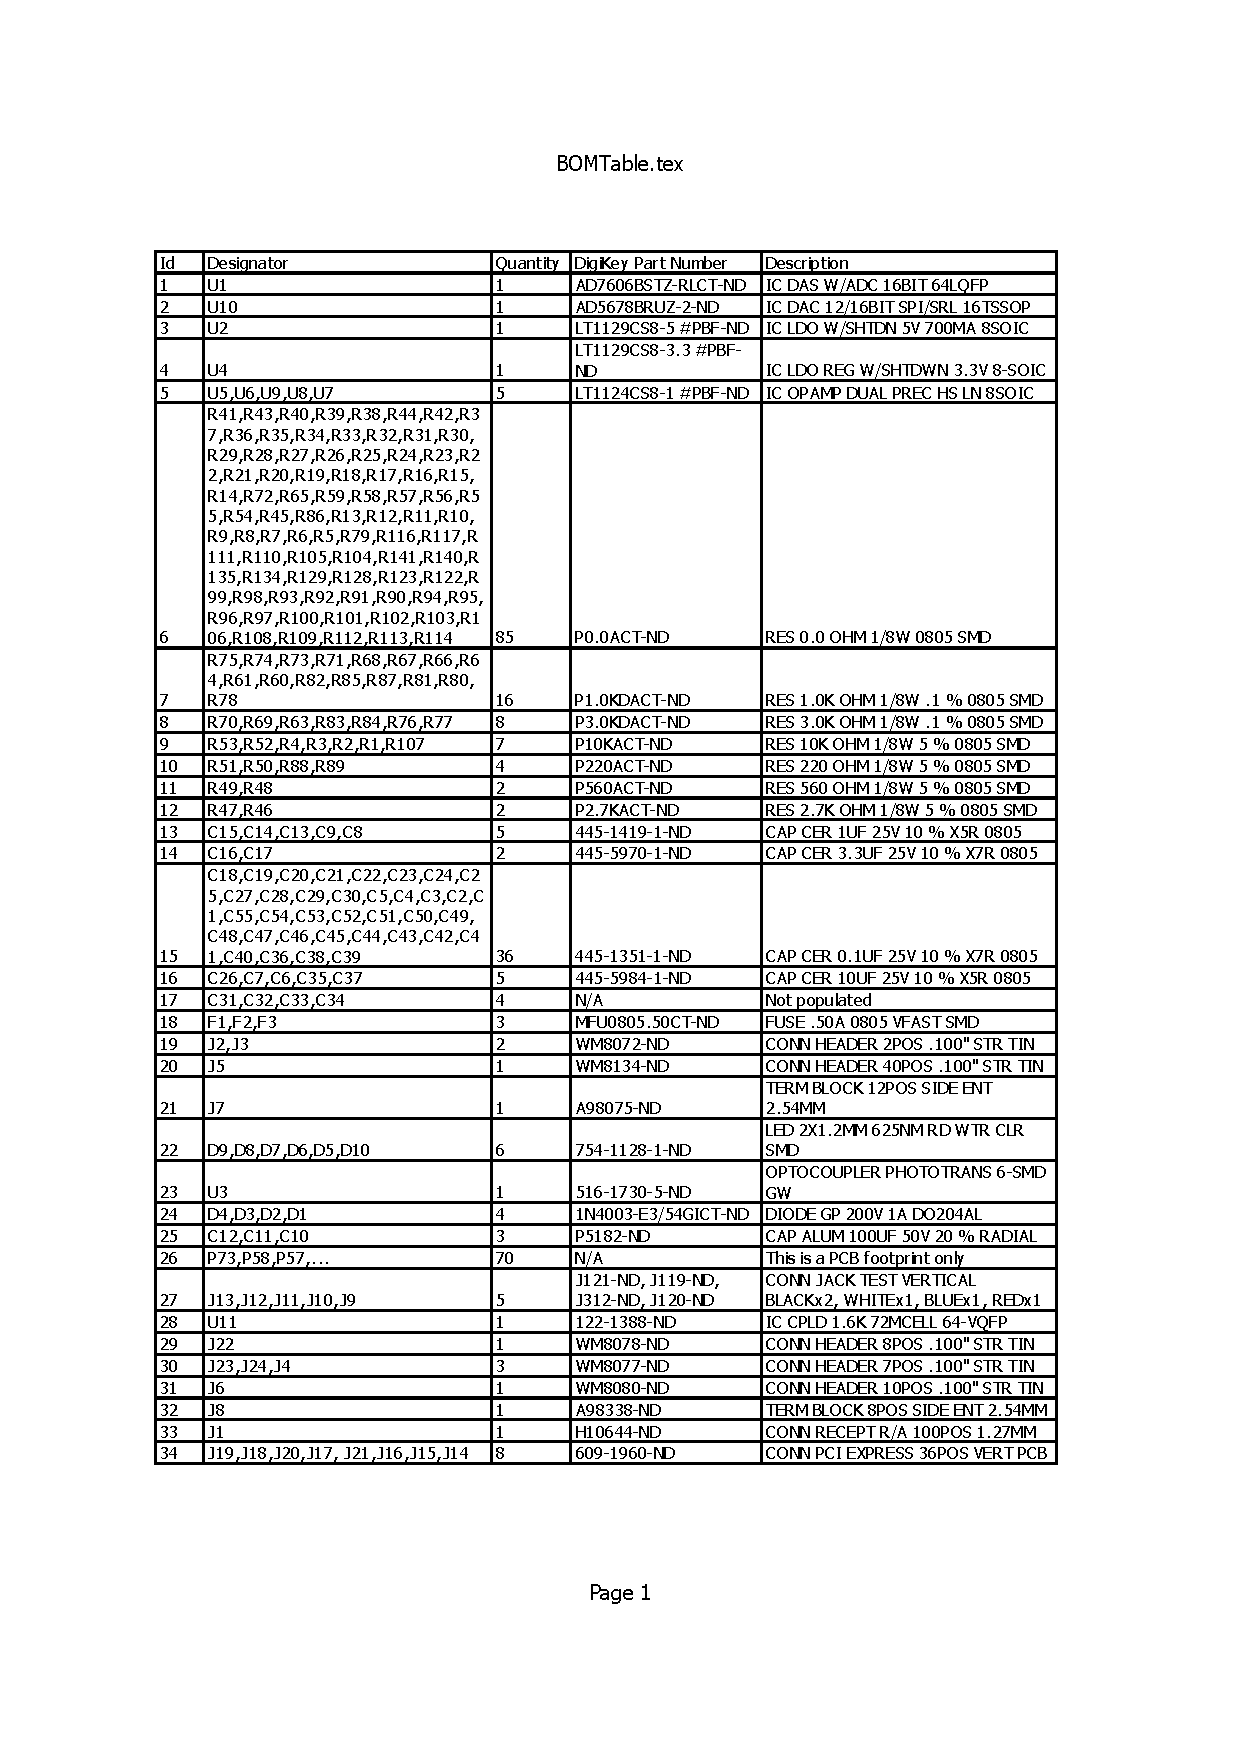
\includegraphics[page=1,trim=1in 1.7in 1.2in 1.5in,clip,width=\textwidth-0.25in ]{./figures/BOMTableLongForm} %[trim=left bottom right top]
\end{tabular}
\caption{Electrophysiology Interface Board Bill of Materials, assembly\label{tab:boma} }
\end{table}
\end{center}

\section{Revision 1.0 Errata}\label{sec:errata}

Table~\ref{tab:errata} is a description of the problems with the first revision of the Electrophysiology Interface Board that require rework of the PCB for it to work as desired or that should be fixed if another board is ordered (Rev1.1)

\begin{singlespace}
\begin{center}
\begin{table}[H]
\begin{tabular}{|l|p{1.5in}|l|p{1.5in}|}
\hline	Affected parts	&Problem 	&Implementation	&Solution\\ \hline
D2	&D2 is forward bias under normal operation, it shorts AGND and {--VA}	&Immediate	&Flip diode around\\ \hline
C13	&Reference isn't on silks	&Next Rev.	&Move reference in Pcbnew\\ \hline
U3/4	&No test point on SHDN of U4	&Next Rev.	&Add test point in Eechema\\ \hline
U4	&Output doesn't drop when in shutdown (capacitors stay charged)	&Next Rev.	&Add load resistor, $220\unit{\Omega}$ tested, try $10\unit{k\Omega}$\\ \hline
P1	&Reference isn't on silks	&Next Rev.	&Move reference in Pcbnew\\ \hline
U11	&JTAG TDI and TDO swapped	&Immediate	&Don't populate R92 and R93, use pads to reroute signal\\ \hline
C1	&Reference isn't on silks	&Next Rev.	&Move reference in Pcbnew\\ \hline
U5/7	&Reference is under part	&Next Rev.	&Move reference in Pcbnew\\ \hline
\end{tabular}
\caption{Electrophysiology Interface Board revision 1.0 errata\label{tab:errata} }
\end{table}
\end{center}
\end{singlespace}

\section{Earthworm Experiment Notes}\label{sec:tips}

\paragraph{Ground Wire} Multiple sources insist that a ground wire is necessary between the stimulating and recording electrodes~\cite{StahlMSEE,Olivo,KuehJellies,EllingerMSEE,Kladt2010}.  In~\cite{Olivo}, it is suggested that one of the dissecting pins may be connected to ground.  In~\cite{Kladt2010}, which is an experiment in which the earthworm is not dissected, a piece of aluminium foil is placed on the earthworm body and connected to ground.  \cite{KuehJellies} implies that a chlorided silver wire is placed under the body of earthworm and connected to ground; this is illustrated in figures~\ref{fig:EWSetup} and~\ref{fig:EWSetupPA}, and it is the setup used to achieve the results in section~\ref{sec:app}.

In some of the first attempts at the experiment, I used a general purpose tin or nickel (I'm not sure which) plated solid copper core hookup wire stripped of its insulation and placed under the earthworm body and connected to ground.  With the plated copper wire, I saw 60Hz noise coming out of the Preamp connected to the recording electrodes.  Switching to chlorided silver wire for the ground wire under the earthworm eliminated the problem.  It was suggested to me by either Dr. Miller or Mr. Mike Ellinger that copper is toxic to cells and should certainly not be used for the recording electrodes, but it seems that plated copper wire should not be used for the ground wire.  It may also be that the tin or nickel plating is toxic to the worm (this is only my supposition).  \cite{Olivo} and~\cite{Kladt2010} appear to successfully use a steel pin and aluminium foil, respectively, as the ground ``wire.''

\paragraph{Response Abnormalities} Another issue that appeared in our attempts at recreating the experiment with earthworm giant axons described in~\cite{StahlMSEE,Olivo,KuehJellies,EllingerMSEE} was trying to recreate the shape (biphasic) and amplitude.  This issue was unrelated to the DASS hardware, specifically, as much of this behavior was observed with a commercial stimulator and a Preamp board from~\cite{BatzerCorsiCrampton}.

The expected biphasic (0V to positive to 0V to negative to 0V) shape of the combined action potentials along the nerve cord, as seen in the lateral response in figure~\ref{fig:EWLatResp}, is due to the relative polarization on the nerve cord between the recording electrodes~\cite{KuehJellies,McGillCAP}.  It is a coincidence that the combined action potential resembles the membrane voltage during a single action potential response.  It was somewhat disconcerting to see that the median response in figures~\ref{fig:EWMedResp} and~\ref{fig:EWLatResp} was monophasic (0V to positive to 0V).  Although, monophasic median and lateral responses were also observed in figure 32 of~\cite{StahlMSEE}.  Also,~\cite{McGillCAP} concerns a similar experiment with the sciatic nerve of a frog, and it says that a nerve cord that is crushed at one of the recording electrode will result in a monophasic response measurement.  I hypothesize that a similar phenomenon could occur in the earthworm's nerve cord.

We also experienced inconsistent results in the amplitude of the response waveforms.  The position of the recording electrodes will affect the amplitude of the response: recording electrodes placed further apart will result in a lower amplitude, as reported in~\cite{KuehJellies,McGillCAP}.  Consequently, it is expected that the responses measure with different earthworms will have different amplitudes.  But, we experienced varying amplitudes with the same worm.   One thing we observed was that when using the commercial Grass SD9 Stimulator set to send stimulation pulses at the same level about 1-5 times per second, the amplitude of the response waveforms were consistent.  If the stimulation were turned off for a time and turned back on, the amplitude of the response would be different.  This causes inconsistent response amplitudes when using the DASS because stimulation pulses are not happening at a consistent rate: the script run on the DASCC might be set to send one stimulation pulse at some amplitude, the results analyzed by the operator, the stimulation amplitude adjusted, and then another stimulation pulse sent.  This means that stimulation pulses are sent at irregular intervals with minutes in between pulses.  Moistening the nerve cord also changed the response amplitude.

Large stimulation artifacts that did not settle before the median response occurred (figure~\ref{fig:settle}), abnormal (not mono or bi-phasic) shapes (figure~\ref{fig:abnormal}), and multiple apparent responses from one stimulus (figure~\ref{fig:multi}) also appeared in the early experiments.  As the issues were being investigated, I focused on improving the biological experimental technique.  Keeping the nerve cord moist with Ringer's solution (as suggested by~\cite{Olivo,KuehJellies}) while also keeping the amount of solution collecting around the worm to a minimum (by wicking excess solution away with paper towel) appears to have kept the aforementioned issues from happening again (since the Aug. 10, 2012 experiments).

\begin{figure}[H]
	\centering 
	\begin{singlespace}
	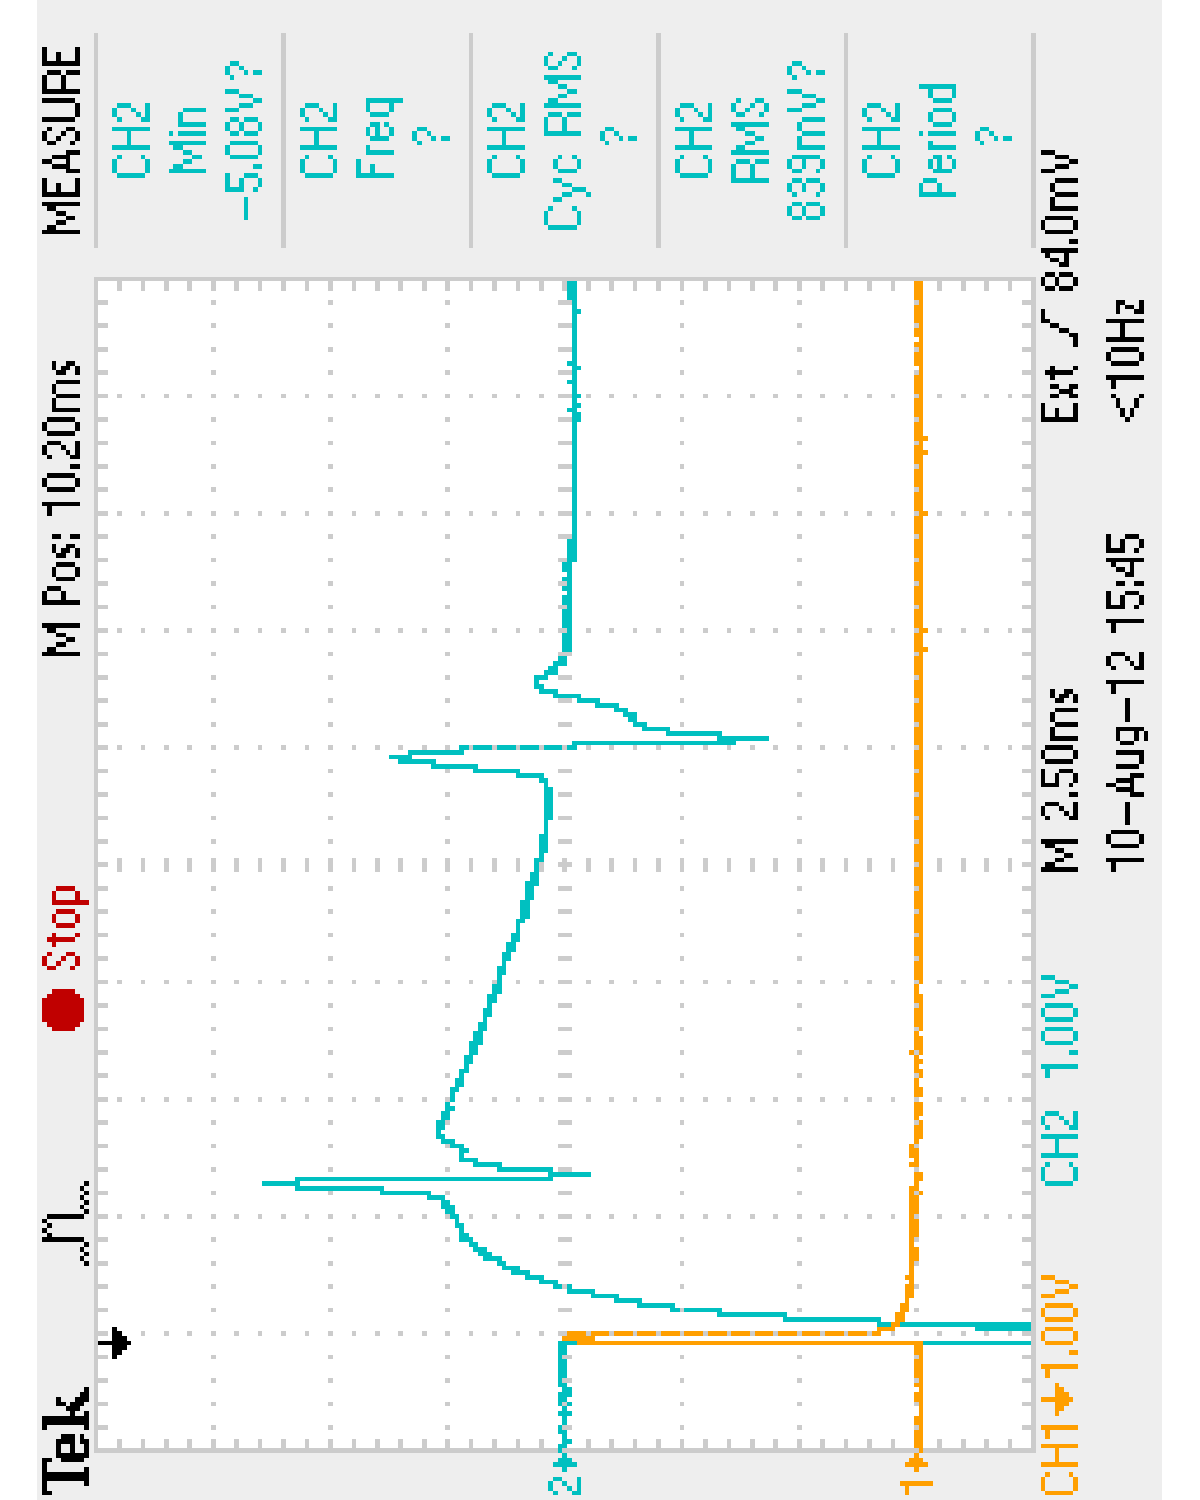
\includegraphics[trim=0 0.1in 0 0.1in,clip,angle=-90,width=0.48\textwidth]{./figures/F0002TEK_settle_120810} %[trim=left bottom right top]
	\caption{ALL0002 Aug. 10, 2012; long stimulus artifact settling time\label{fig:settle}}
	\end{singlespace}
\end{figure}

\begin{figure}[H]
	\centering 
	\begin{singlespace}
	\begin{subfigure}[b]{0.48\textwidth}
		\centering 
		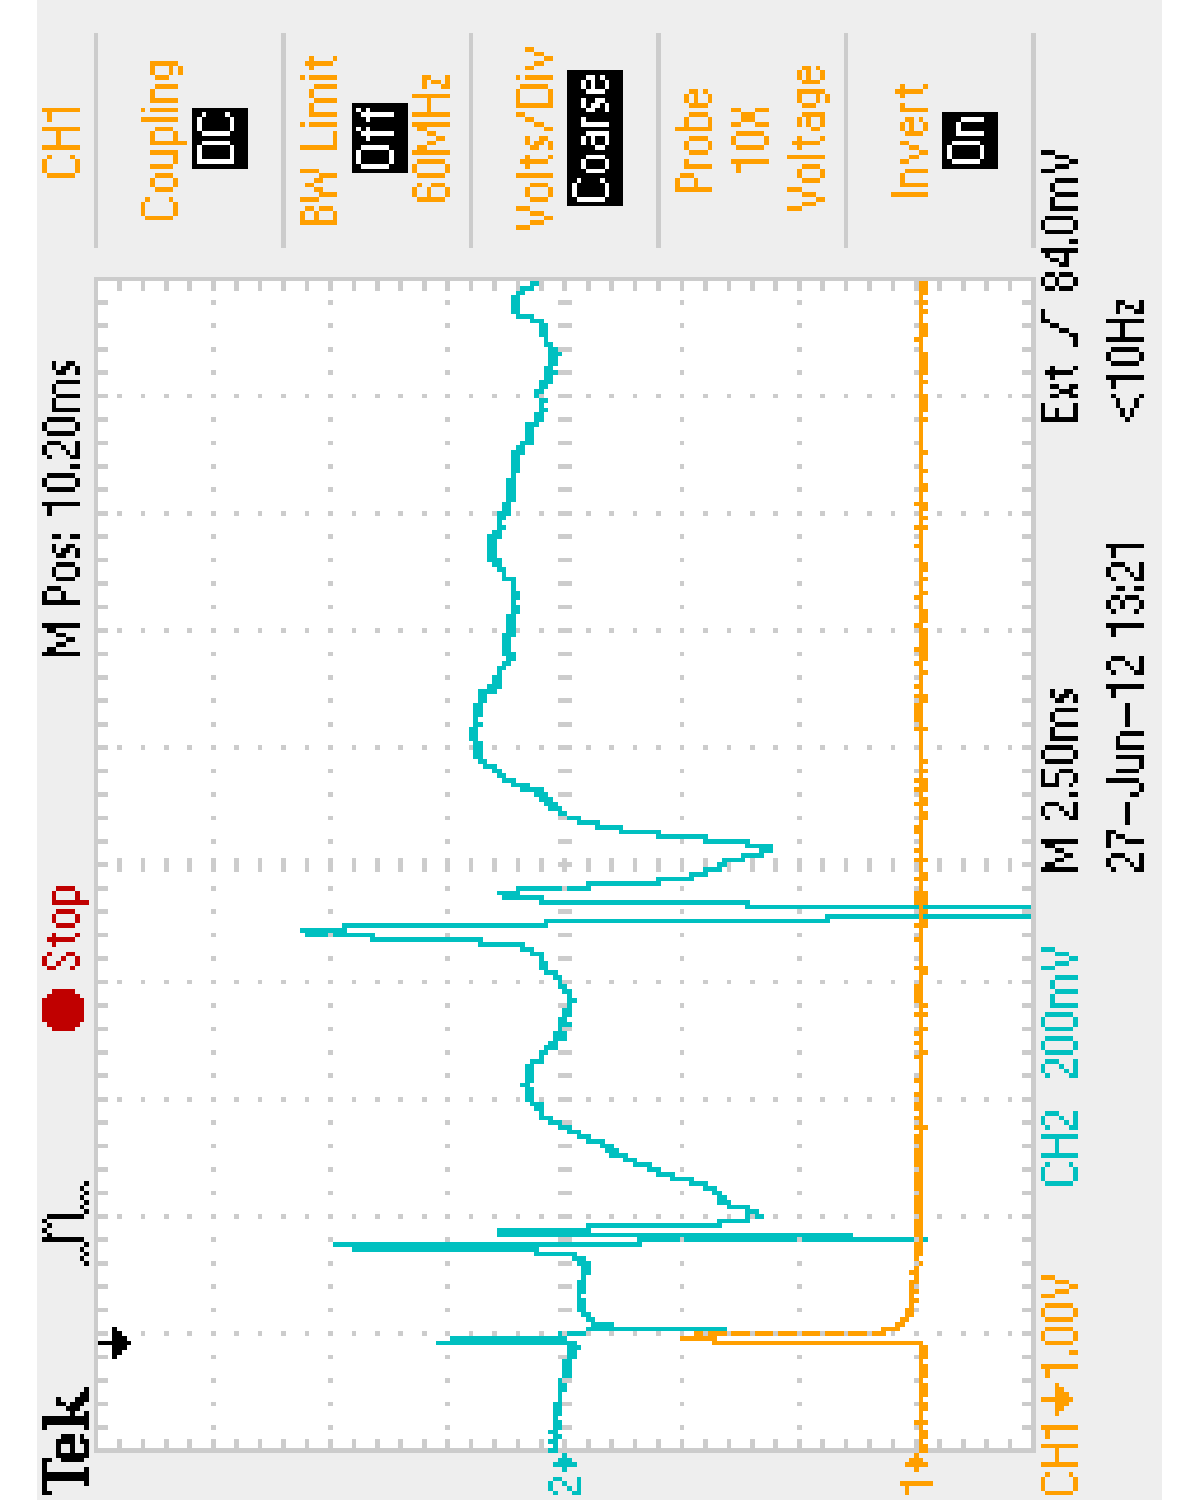
\includegraphics[trim=0 0.1in 0 0.1in,clip,angle=-90,width=\textwidth]{./figures/F0000TEK_abnorm_120627} %[trim=left bottom right top]
	\caption{ALL0000 June 27, 2012}
	\end{subfigure}
	~
	\begin{subfigure}[b]{0.48\textwidth}
		\centering 
		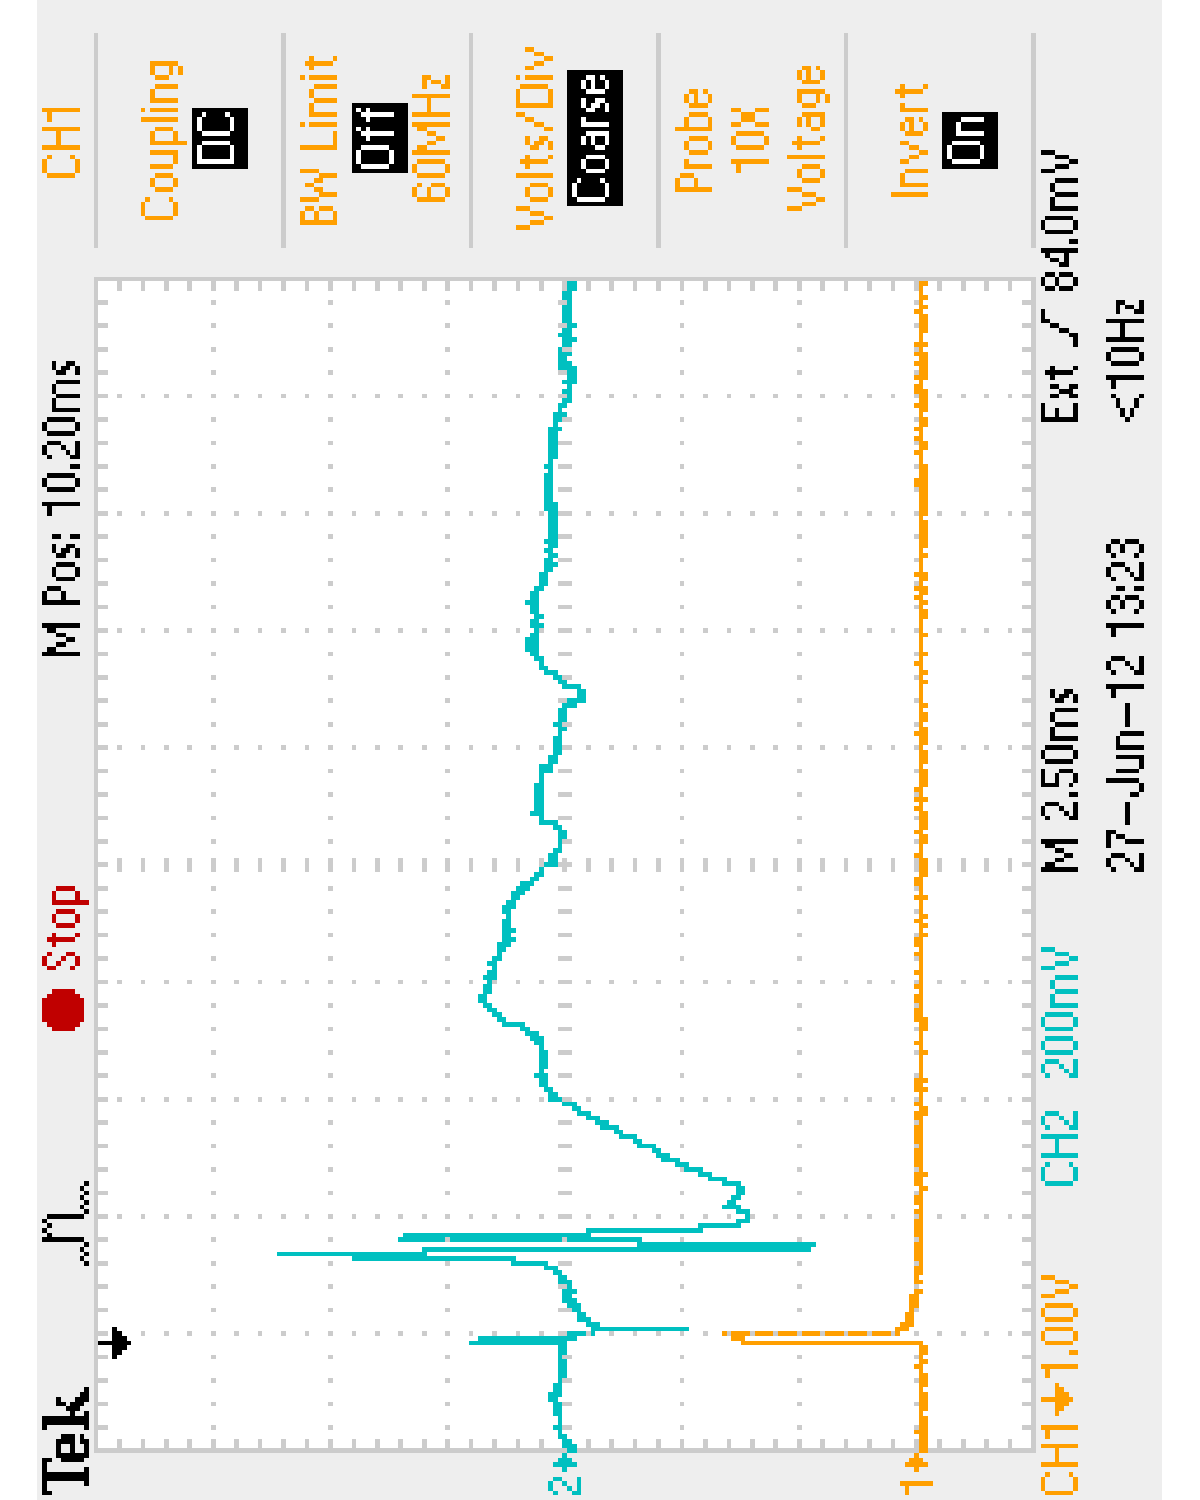
\includegraphics[trim=0 0.1in 0 0.1in,clip,clip,angle=-90,width=\textwidth]{./figures/F0001TEK_abnorm_120627} %[trim=left bottom right top]
	\caption{ALL0001 June 27, 2012}
	\end{subfigure}
	\caption{Abnormally shaped earthworm giant axon responses\label{fig:abnormal}}
	\end{singlespace}
\end{figure}

\begin{figure}[H]
	\centering 
	\begin{singlespace}
	\begin{subfigure}[b]{0.48\textwidth}
		\centering 
		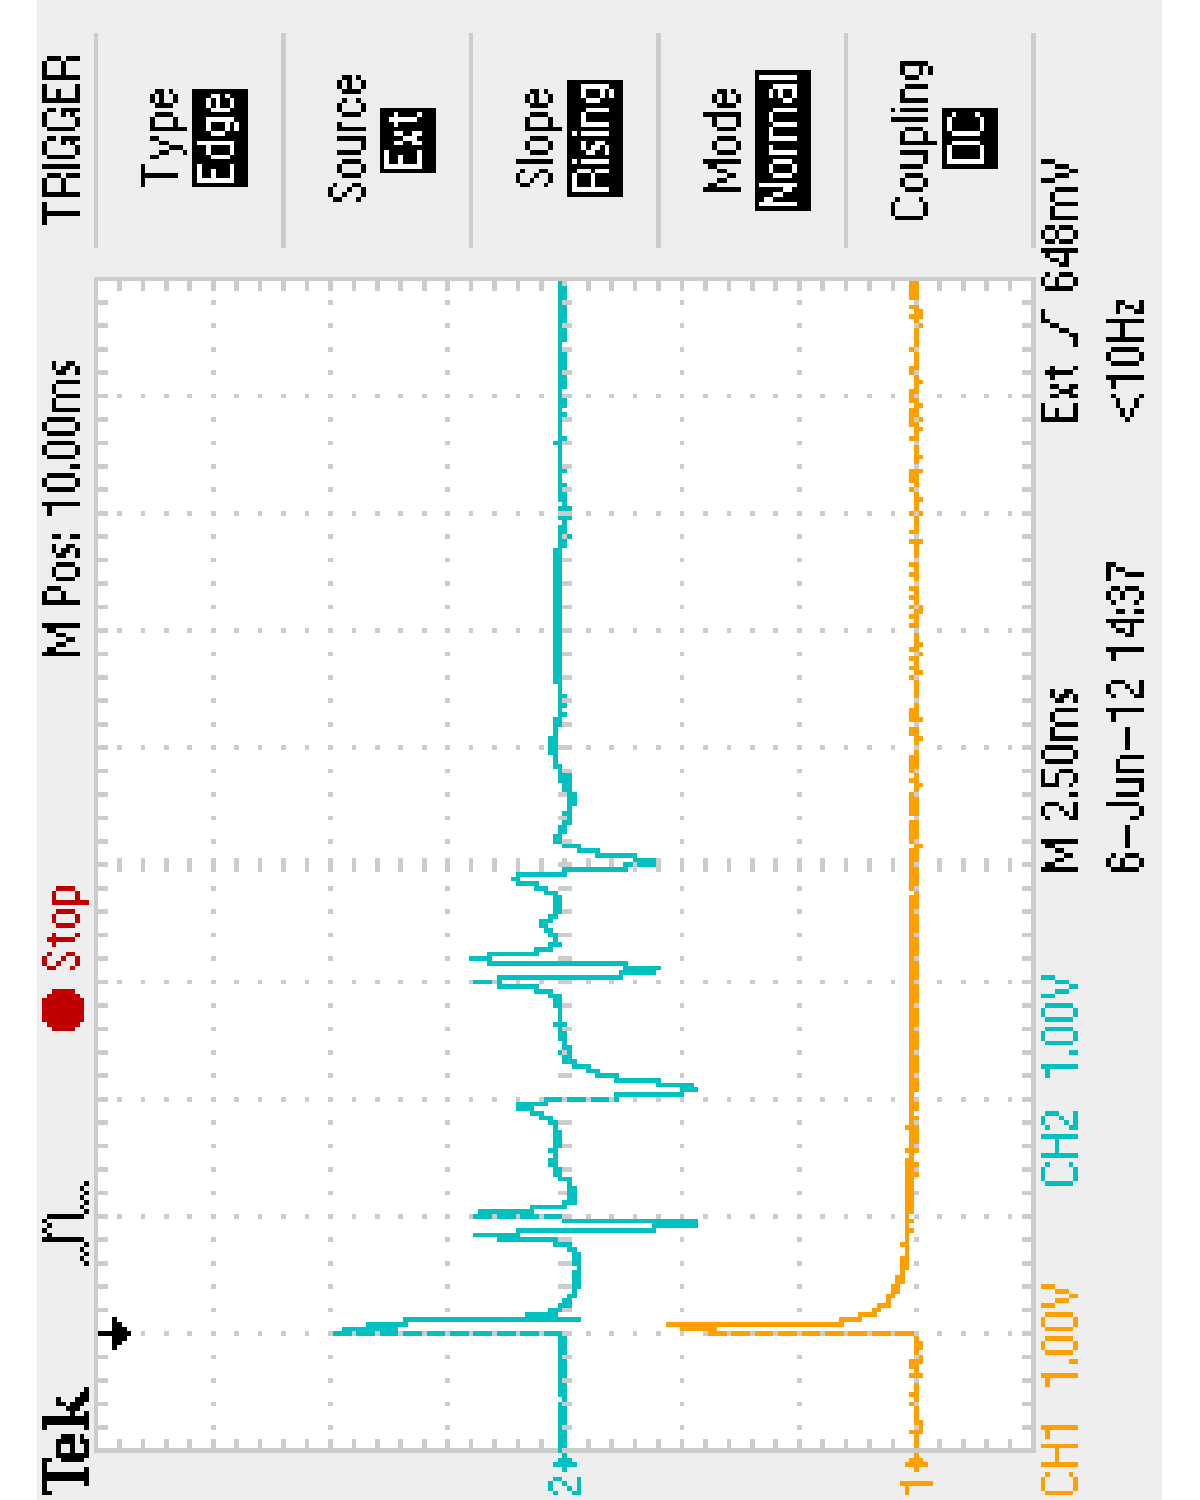
\includegraphics[trim=0 0.1in 0 0.1in,clip,angle=-90,width=\textwidth]{./figures/F0003TEK_multi_120606} %[trim=left bottom right top]
	\caption{ALL0003 June 06, 2012}
	\end{subfigure}
	~
	\begin{subfigure}[b]{0.48\textwidth}
		\centering 
		\resizebox{\textwidth}{!}{% GNUPLOT: LaTeX picture with Postscript
\begingroup
  \makeatletter
  \providecommand\color[2][]{%
    \GenericError{(gnuplot) \space\space\space\@spaces}{%
      Package color not loaded in conjunction with
      terminal option `colourtext'%
    }{See the gnuplot documentation for explanation.%
    }{Either use 'blacktext' in gnuplot or load the package
      color.sty in LaTeX.}%
    \renewcommand\color[2][]{}%
  }%
  \providecommand\includegraphics[2][]{%
    \GenericError{(gnuplot) \space\space\space\@spaces}{%
      Package graphicx or graphics not loaded%
    }{See the gnuplot documentation for explanation.%
    }{The gnuplot epslatex terminal needs graphicx.sty or graphics.sty.}%
    \renewcommand\includegraphics[2][]{}%
  }%
  \providecommand\rotatebox[2]{#2}%
  \@ifundefined{ifGPcolor}{%
    \newif\ifGPcolor
    \GPcolorfalse
  }{}%
  \@ifundefined{ifGPblacktext}{%
    \newif\ifGPblacktext
    \GPblacktexttrue
  }{}%
  % define a \g@addto@macro without @ in the name:
  \let\gplgaddtomacro\g@addto@macro
  % define empty templates for all commands taking text:
  \gdef\gplbacktext{}%
  \gdef\gplfronttext{}%
  \makeatother
  \ifGPblacktext
    % no textcolor at all
    \def\colorrgb#1{}%
    \def\colorgray#1{}%
  \else
    % gray or color?
    \ifGPcolor
      \def\colorrgb#1{\color[rgb]{#1}}%
      \def\colorgray#1{\color[gray]{#1}}%
      \expandafter\def\csname LTw\endcsname{\color{white}}%
      \expandafter\def\csname LTb\endcsname{\color{black}}%
      \expandafter\def\csname LTa\endcsname{\color{black}}%
      \expandafter\def\csname LT0\endcsname{\color[rgb]{1,0,0}}%
      \expandafter\def\csname LT1\endcsname{\color[rgb]{0,1,0}}%
      \expandafter\def\csname LT2\endcsname{\color[rgb]{0,0,1}}%
      \expandafter\def\csname LT3\endcsname{\color[rgb]{1,0,1}}%
      \expandafter\def\csname LT4\endcsname{\color[rgb]{0,1,1}}%
      \expandafter\def\csname LT5\endcsname{\color[rgb]{1,1,0}}%
      \expandafter\def\csname LT6\endcsname{\color[rgb]{0,0,0}}%
      \expandafter\def\csname LT7\endcsname{\color[rgb]{1,0.3,0}}%
      \expandafter\def\csname LT8\endcsname{\color[rgb]{0.5,0.5,0.5}}%
    \else
      % gray
      \def\colorrgb#1{\color{black}}%
      \def\colorgray#1{\color[gray]{#1}}%
      \expandafter\def\csname LTw\endcsname{\color{white}}%
      \expandafter\def\csname LTb\endcsname{\color{black}}%
      \expandafter\def\csname LTa\endcsname{\color{black}}%
      \expandafter\def\csname LT0\endcsname{\color{black}}%
      \expandafter\def\csname LT1\endcsname{\color{black}}%
      \expandafter\def\csname LT2\endcsname{\color{black}}%
      \expandafter\def\csname LT3\endcsname{\color{black}}%
      \expandafter\def\csname LT4\endcsname{\color{black}}%
      \expandafter\def\csname LT5\endcsname{\color{black}}%
      \expandafter\def\csname LT6\endcsname{\color{black}}%
      \expandafter\def\csname LT7\endcsname{\color{black}}%
      \expandafter\def\csname LT8\endcsname{\color{black}}%
    \fi
  \fi
  \setlength{\unitlength}{0.0500bp}%
  \begin{picture}(11520.00,8640.00)%
    \gplgaddtomacro\gplbacktext{%
      \colorrgb{0.00,0.00,0.00}%
      \put(1377,5044){\makebox(0,0)[r]{\strut{}-6}}%
      \colorrgb{0.00,0.00,0.00}%
      \put(1377,5535){\makebox(0,0)[r]{\strut{}-4}}%
      \colorrgb{0.00,0.00,0.00}%
      \put(1377,6026){\makebox(0,0)[r]{\strut{}-2}}%
      \colorrgb{0.00,0.00,0.00}%
      \put(1377,6518){\makebox(0,0)[r]{\strut{}0}}%
      \colorrgb{0.00,0.00,0.00}%
      \put(1377,7009){\makebox(0,0)[r]{\strut{}2}}%
      \colorrgb{0.00,0.00,0.00}%
      \put(1377,7500){\makebox(0,0)[r]{\strut{}4}}%
      \colorrgb{0.00,0.00,0.00}%
      \put(1377,7991){\makebox(0,0)[r]{\strut{}6}}%
      \colorrgb{0.00,0.00,0.00}%
      \put(1497,4844){\makebox(0,0){\strut{}0}}%
      \colorrgb{0.00,0.00,0.00}%
      \put(3282,4844){\makebox(0,0){\strut{}50}}%
      \colorrgb{0.00,0.00,0.00}%
      \put(5068,4844){\makebox(0,0){\strut{}100}}%
      \colorrgb{0.00,0.00,0.00}%
      \put(6853,4844){\makebox(0,0){\strut{}150}}%
      \colorrgb{0.00,0.00,0.00}%
      \put(8639,4844){\makebox(0,0){\strut{}200}}%
      \colorrgb{0.00,0.00,0.00}%
      \put(10424,4844){\makebox(0,0){\strut{}250}}%
      \colorrgb{0.00,0.00,0.00}%
      \put(917,6517){\rotatebox{90}{\makebox(0,0){\strut{}Voltage ($V$)}}}%
      \colorrgb{0.00,0.00,0.00}%
      \put(5960,4544){\makebox(0,0){\strut{}Time ($ms$)}}%
      \csname LTb\endcsname%
      \put(5960,8291){\makebox(0,0){\strut{}Multiple Stimulations}}%
    }%
    \gplgaddtomacro\gplfronttext{%
      \colorrgb{0.00,0.00,0.00}%
      \put(6139,5781){\makebox(0,0)[l]{\strut{}Stimulus Artifact}}%
      \put(6496,7254){\makebox(0,0)[l]{\strut{}Multiple Lateral Giant Responses?}}%
    }%
    \gplgaddtomacro\gplbacktext{%
      \colorrgb{0.00,0.00,0.00}%
      \put(1377,950){\makebox(0,0)[r]{\strut{}-6}}%
      \colorrgb{0.00,0.00,0.00}%
      \put(1377,1441){\makebox(0,0)[r]{\strut{}-4}}%
      \colorrgb{0.00,0.00,0.00}%
      \put(1377,1932){\makebox(0,0)[r]{\strut{}-2}}%
      \colorrgb{0.00,0.00,0.00}%
      \put(1377,2424){\makebox(0,0)[r]{\strut{}0}}%
      \colorrgb{0.00,0.00,0.00}%
      \put(1377,2915){\makebox(0,0)[r]{\strut{}2}}%
      \colorrgb{0.00,0.00,0.00}%
      \put(1377,3406){\makebox(0,0)[r]{\strut{}4}}%
      \colorrgb{0.00,0.00,0.00}%
      \put(1377,3897){\makebox(0,0)[r]{\strut{}6}}%
      \colorrgb{0.00,0.00,0.00}%
      \put(1497,750){\makebox(0,0){\strut{}-5}}%
      \colorrgb{0.00,0.00,0.00}%
      \put(3282,750){\makebox(0,0){\strut{}0}}%
      \colorrgb{0.00,0.00,0.00}%
      \put(5068,750){\makebox(0,0){\strut{}5}}%
      \colorrgb{0.00,0.00,0.00}%
      \put(6853,750){\makebox(0,0){\strut{}10}}%
      \colorrgb{0.00,0.00,0.00}%
      \put(8639,750){\makebox(0,0){\strut{}15}}%
      \colorrgb{0.00,0.00,0.00}%
      \put(10424,750){\makebox(0,0){\strut{}20}}%
      \colorrgb{0.00,0.00,0.00}%
      \put(917,2423){\rotatebox{90}{\makebox(0,0){\strut{}Voltage ($V$)}}}%
      \colorrgb{0.00,0.00,0.00}%
      \put(5960,450){\makebox(0,0){\strut{}Time ($ms$)}}%
      \csname LTb\endcsname%
      \put(5960,4197){\makebox(0,0){\strut{}Multiple Stimulations, Zoom}}%
    }%
    \gplgaddtomacro\gplfronttext{%
      \colorrgb{0.00,0.00,0.00}%
      \put(4443,1564){\makebox(0,0)[l]{\strut{}Stimulus Artifact}}%
      \put(5104,3222){\makebox(0,0)[l]{\strut{}Median Giant Response}}%
      \put(8728,2853){\makebox(0,0)[l]{\strut{}Lateral Giant Response?}}%
    }%
    \gplbacktext
    \put(0,0){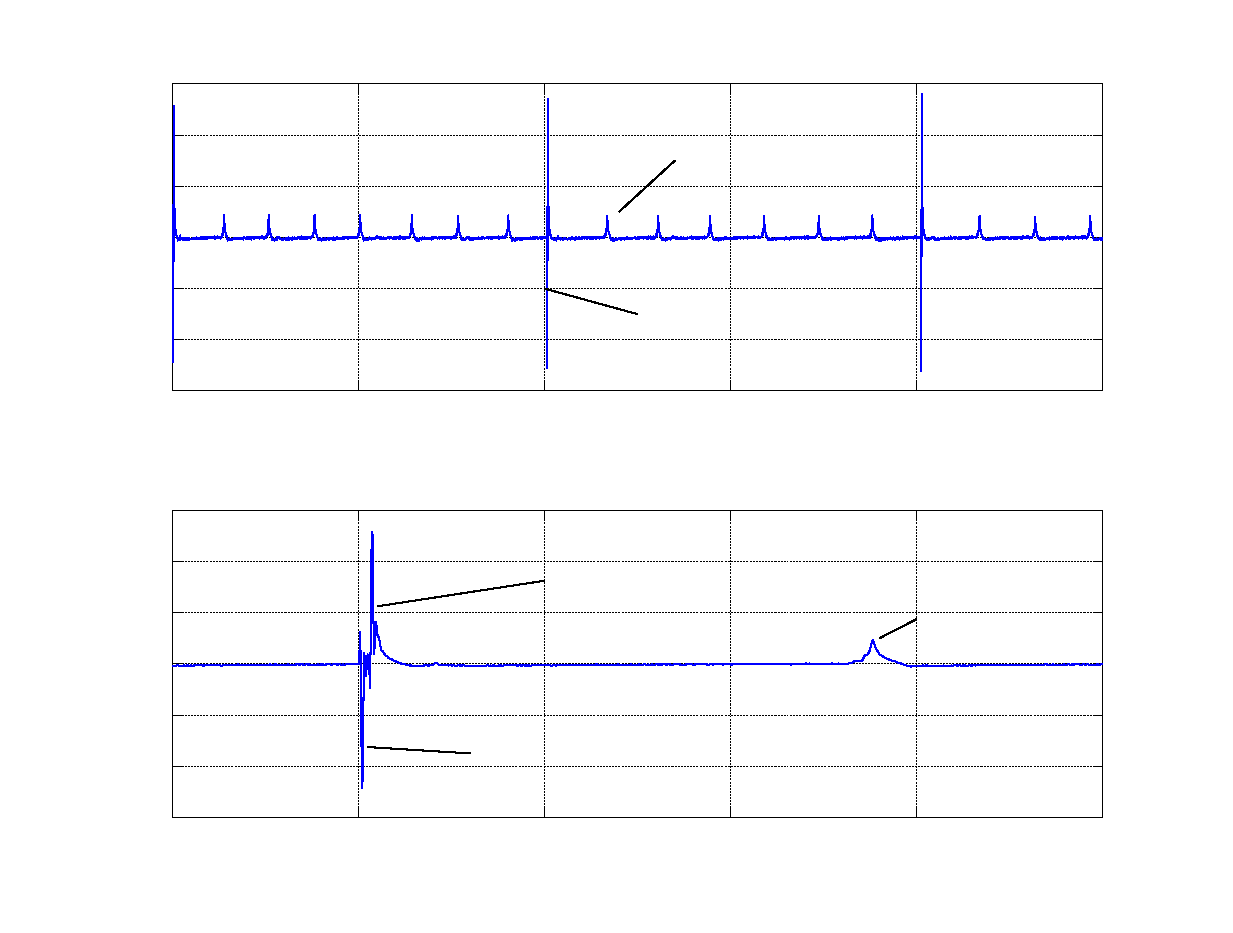
\includegraphics{MULTIresponse}}%
    \gplfronttext
  \end{picture}%
\endgroup
}
	\caption{data\_out0-multi1 May 16, 2012}
	\end{subfigure}
	\caption{Multiple earthworm giant axon responses per single stimulus\label{fig:multi}}
	\end{singlespace}
\end{figure}

\paragraph{Silver Wire Size} In an attempt to save money, larger diameter silver wire than is recommended in~\cite{KuehJellies} was used to perform the earthworm experiment.  The following is an excerpt from an email composed by me and sent to Dr.~Damon A.~Miller and Mr.~Mike Ellinger on April 22, 2012 summarizing the cost savings:

\begin{quotation}
For the silver wire,~\cite{KuehJellies} says to use 0.25mm diameter wire from Warner Instruments.  It looks like it can be bought here:  \url{http://www.warneronline.com/product_info.cfm?ID=280&CFID=6793639&CFTOKEN=40541278}

Their silver wire is 99.99\% pure, and under ``pricing and ordering,'' 2 meters of 0.25mm diameter wire costs \$24 not including shipping plus there's a \$10 charge for having an order of less than \$75.

I found another website that sells 99.99\% 0.635mm (0.025in) wire at \$3.00/ft.  Which means we could get 6ft. for \~\$24 including shipping or \~\$15 for 3ft.  Link: \url{http://www.ccsilver.com/silver/superfines.html}

Yet another website sells 6ft. of 99.9\% 0.025mm wire for \~\$10 including shipping.  Link: \url{http://www.ottofrei.com/store/product.php?productid=21270&cat=3847&page=1} (dead)

To sum up, we can get the original medical grade, 99.99\% purity wire in the same diameter for $>$\$35, we can get the same purity wire but with 2.5 times the diameter for \$15, or we can get 99.9\% wire in the same diameter as the experiment for \$10.

I'm thinking the 99.99\% 0.635mm wire for \$15 would be an acceptable solution.
\end{quotation}

Many of the anomalies in shape and amplitude mentioned in the previous section were observed while using the 0.635mm wire from C.C.~Silver for the recording electrodes.  To eliminate the wire diameter as a factor in those anomalies, the 0.25mm diameter wire from Warner Instruments specified by~\cite{KuehJellies} was purchased and compared with the 0.635mm wire.  Both wire sizes were chlorided and an earthworm was prepared.  The commercial stimulator was used along with a Preamp from~\cite{BatzerCorsiCrampton} connected to an oscilloscope.  Figure~\ref{fig:30to22} shows a 3.5V stimulation with response recorded first using the 0.25mm wire from Warner Instruments, then using the 0.635mm wire from C.C.~Silver.  Figure~\ref{fig:22to30} shows a 3.75V stimulation with response recorded first using the 0.635mm wire, then using the 0.25mm wire.

\begin{figure}[H]
	\centering 
	\begin{singlespace}
	\begin{subfigure}[b]{0.48\textwidth}
		\centering 
		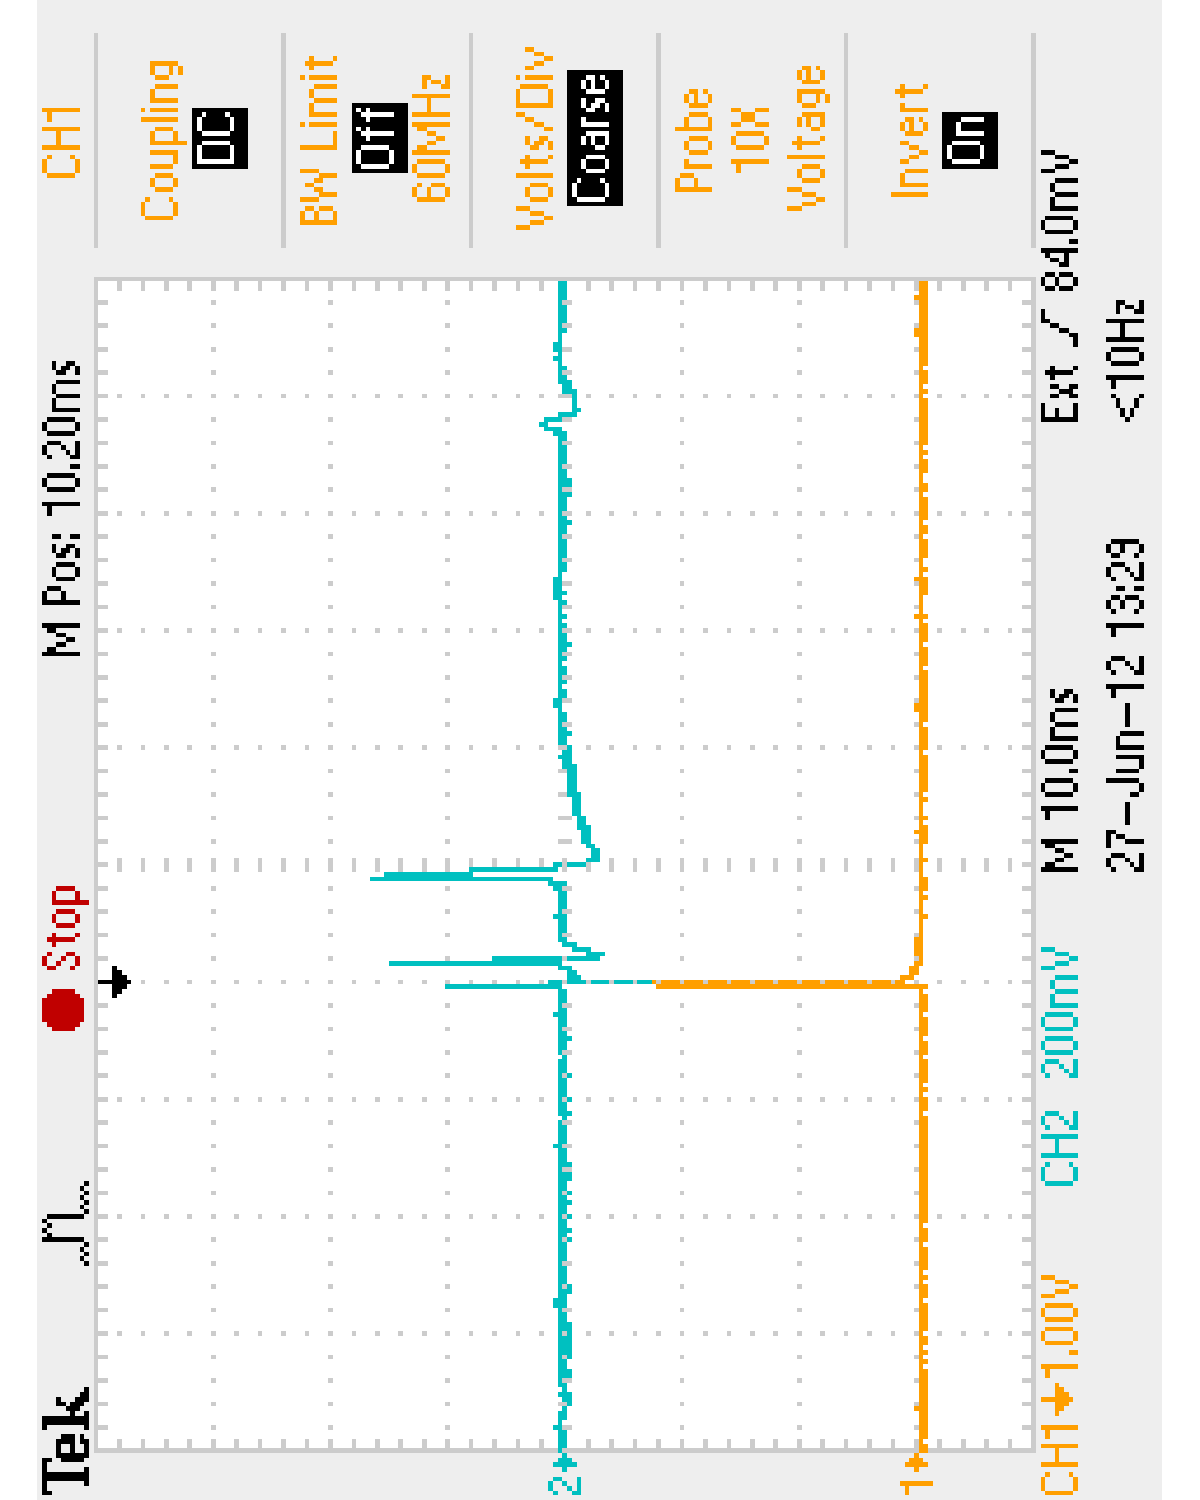
\includegraphics[trim=0 0.1in 0 0.1in,clip,angle=-90,width=\textwidth]{./figures/F0004TEK_30a_120627} %[trim=left bottom right top]
	\caption{ALL0004 June 27, 2012; 0.25mm wire; 3.5V stimulus}
	\end{subfigure}
	~
	\begin{subfigure}[b]{0.48\textwidth}
		\centering 
		\includegraphics[trim=0 0.1in 0 0.1in,clip,angle=-90,width=\textwidth]{./figures/F0005TEK_22a_120627} %[trim=left bottom right top]
	\caption{ALL0005 June 27, 2012; 0.635mm wire; 3.5V stimulus}
	\end{subfigure}
	\caption{Recording electrode silver wire comparison: 0.25mm to 0.635mm\label{fig:30to22}}
	\end{singlespace}
\end{figure}
	
\begin{figure}[H]
	\centering 
	\begin{singlespace}
	\begin{subfigure}[b]{0.48\textwidth}
		\centering 
		\includegraphics[trim=0 0.1in 0 0.1in,clip,angle=-90,width=\textwidth]{./figures/F0006TEK_22b_120627} %[trim=left bottom right top]
	\caption{ALL0006 June 27, 2012; 0.635mm wire; 3.75V stimulus}
	\end{subfigure}
	~
	\begin{subfigure}[b]{0.48\textwidth}
		\centering 
		\includegraphics[trim=0 0.1in 0 0.1in,clip,angle=-90,width=\textwidth]{./figures/F0007TEK_30b_120627} %[trim=left bottom right top]
	\caption{ALL0007 June 27, 2012; 0.25mm wire; 3.5V stimulus}
	\end{subfigure}
	\caption{Recording electrode silver wire comparison: 0.635mm to 0.25mm\label{fig:22to30}}
	\end{singlespace}
\end{figure}

Anomalies in shape and amplitude were experienced with both diameter wires, during the experiment.  The figures show that similar shapes could be observed with both diameter wires.  This led me to the conclusion that wire diameter was not the cause of the difficulties examined in the previous section.


\section{GitHub Repository}

A GitHub repository~\cite{BatzerRepo} has been created that contains the source files and documentation from the companion thesis~\cite{BatzerMSEE}; experimental data and pictures from work done for section~\ref{sec:results}; KiCAD schematic, layout, and library files for the Electrophysiology Interface board; and the \LaTeX source for this thesis.

\newpage

\begin{singlespace} 
\bibliographystyle{IEEEtran}

%Add references to table of contents page
\phantomsection
\addcontentsline{toc}{section}{References}

\bibliography{ref}
\end{singlespace}

\end{document}
